\documentclass[a4paper]{oblivoir}
\usepackage{amsmath,amssymb,kotex,kswrapfig,mdframed,tabto,paralist,graphicx}
\usepackage{fapapersize}
\usefapapersize{210mm,297mm,10mm,*,10mm,*}

%%% Counters
\newcounter{num}

%%% Commands
\newcommand\defi[1]
{\bigskip\par\noindent\stepcounter{num} \textbf{정의 \thenum) #1}\par\noindent}
\newcommand\theo[1]
{\bigskip\par\noindent\stepcounter{num} \textbf{정리 \thenum) #1}\par\noindent}
\newcommand\exam[1]
{\bigskip\par\noindent\stepcounter{num} \textbf{예시 \thenum) #1}\par\noindent}
\newcommand\prob[1]
{\bigskip\par\noindent\stepcounter{num} \textbf{문제 \thenum) #1}\par\noindent}

\newcommand\pb[1]{\ensuremath{\fbox{\phantom{#1}}}}

\newcommand\ba{\ensuremath{\:|\:}}

\newcommand\procedure[1]{\begin{mdframed}\vspace{#1\textheight}\end{mdframed}\bigskip}

\newcommand\an[1]{\bigskip\par\noindent\textbf{문제 #1)}\par\noindent}

%%% Meta Commands
\let\oldsection\section
\renewcommand\section{\clearpage\oldsection}

\let\emph\textsf

%%% Title
\title{그래프 그리기 : 이차함수}
\date{\today}
\author{}

\begin{document}
\maketitle

\begin{minipage}{0.45\textwidth}\centering
\(y=x^2\)
\par\bigskip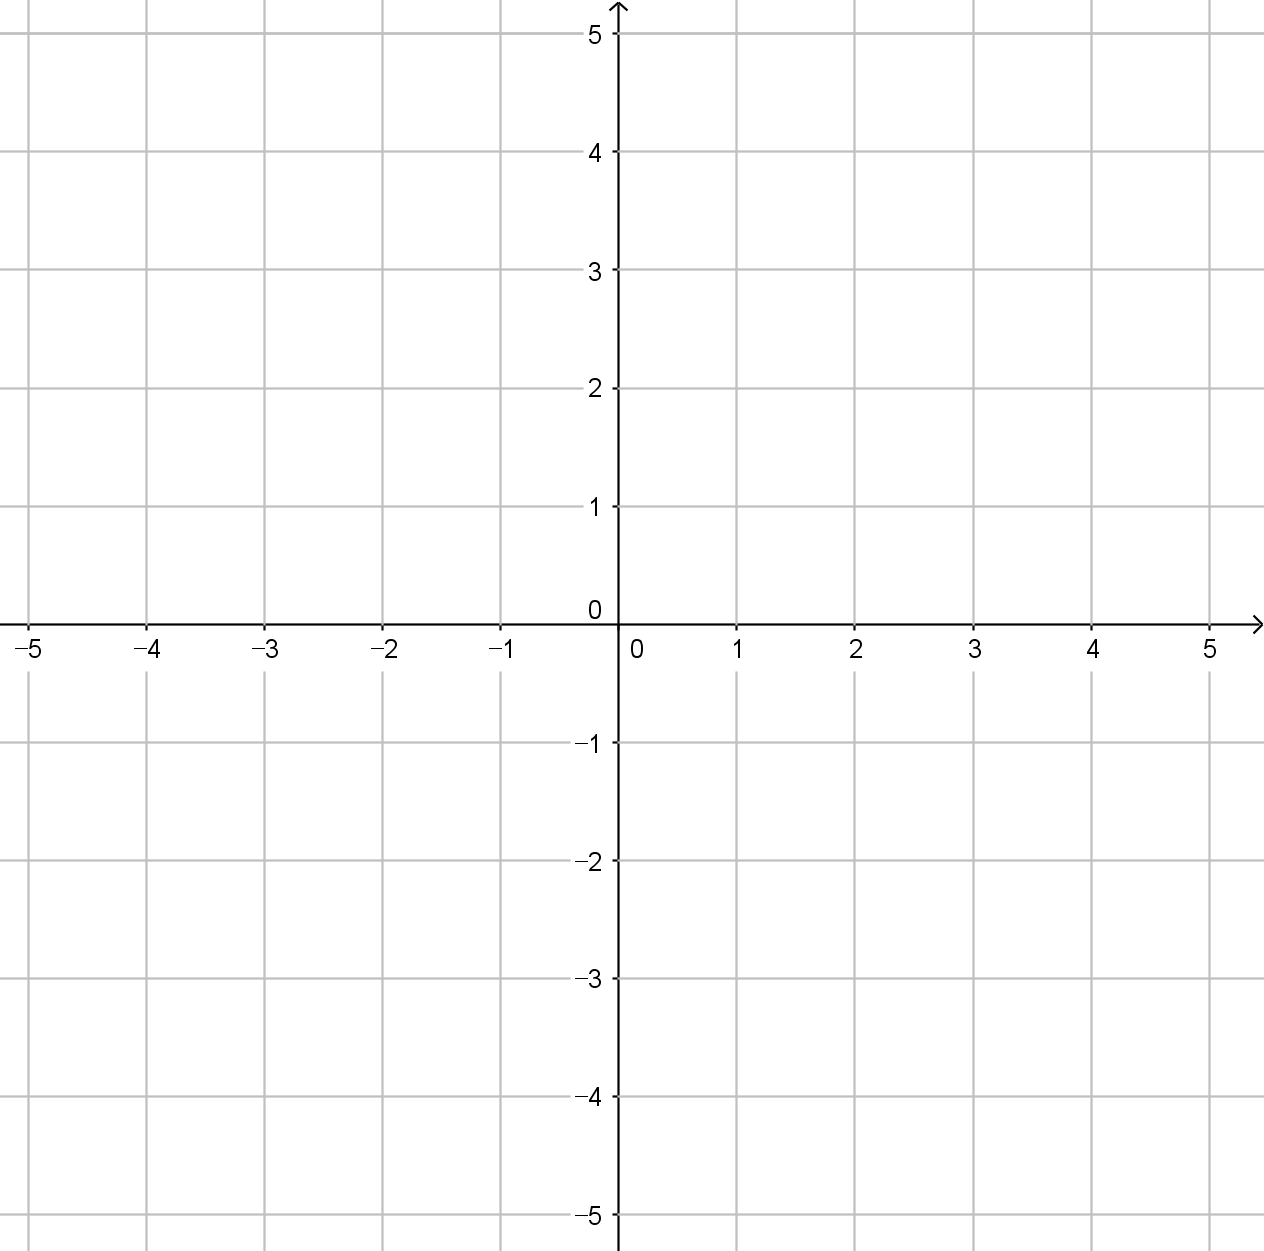
\includegraphics[width=0.9\textwidth]{55}
\end{minipage}
\begin{minipage}{0.45\textwidth}\centering
\(y=-x^2\)
\par\bigskip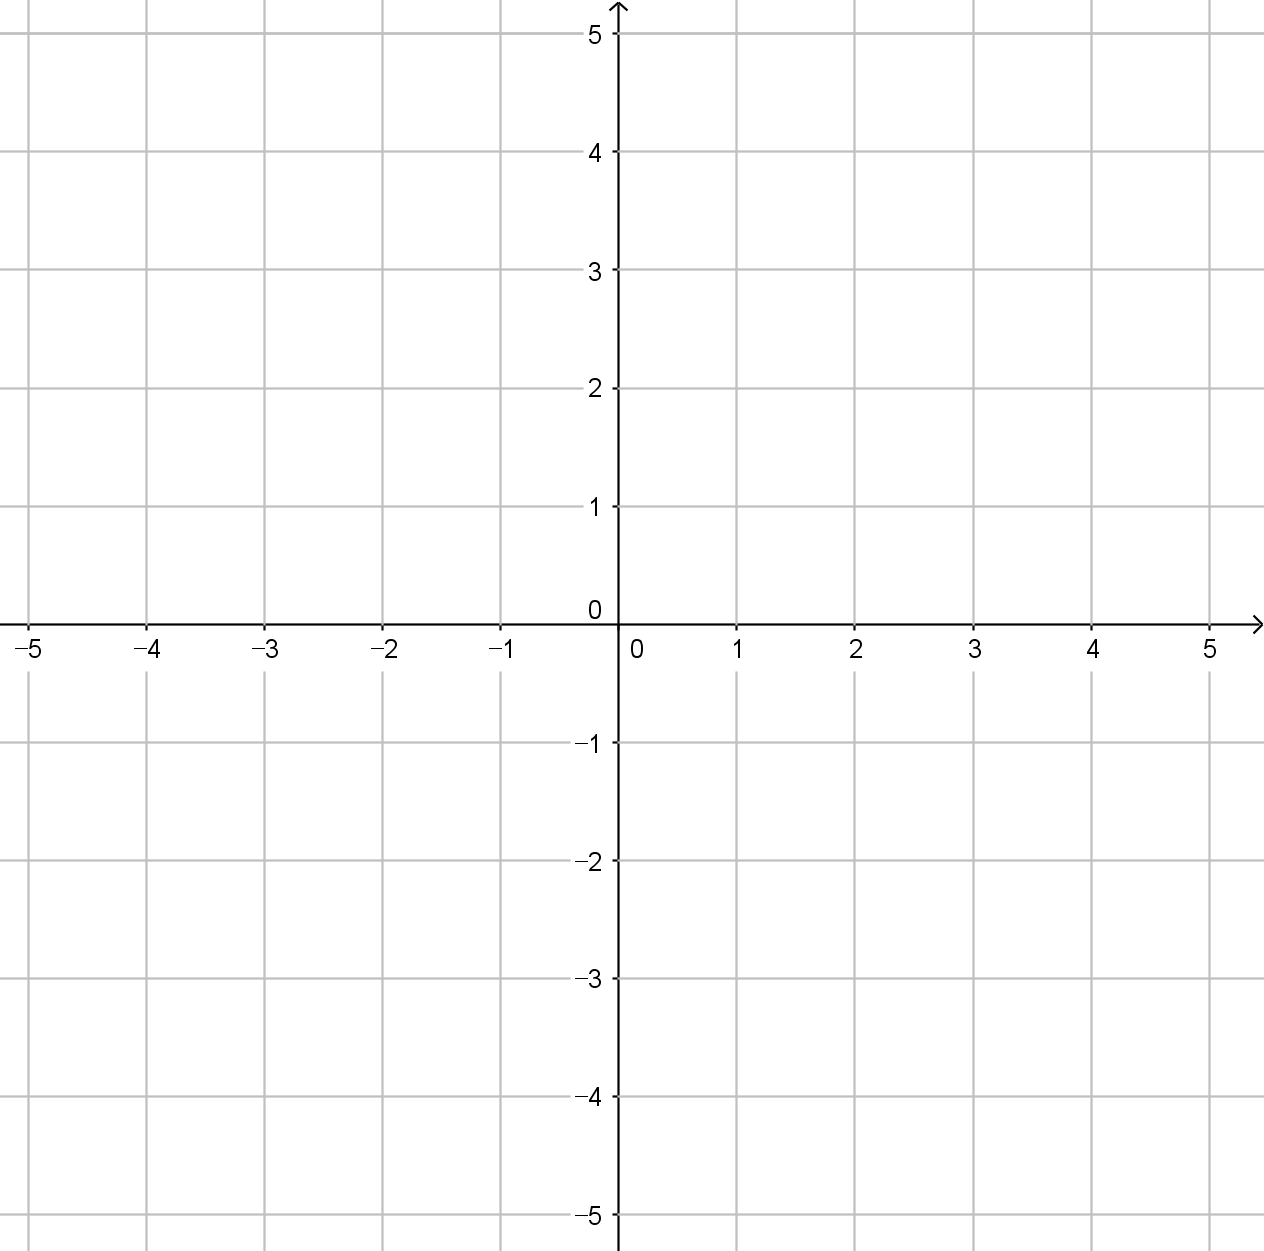
\includegraphics[width=0.9\textwidth]{55}
\end{minipage}\bigskip\bigskip\par
\begin{minipage}{0.45\textwidth}\centering
\(y=2x^2\)
\par\bigskip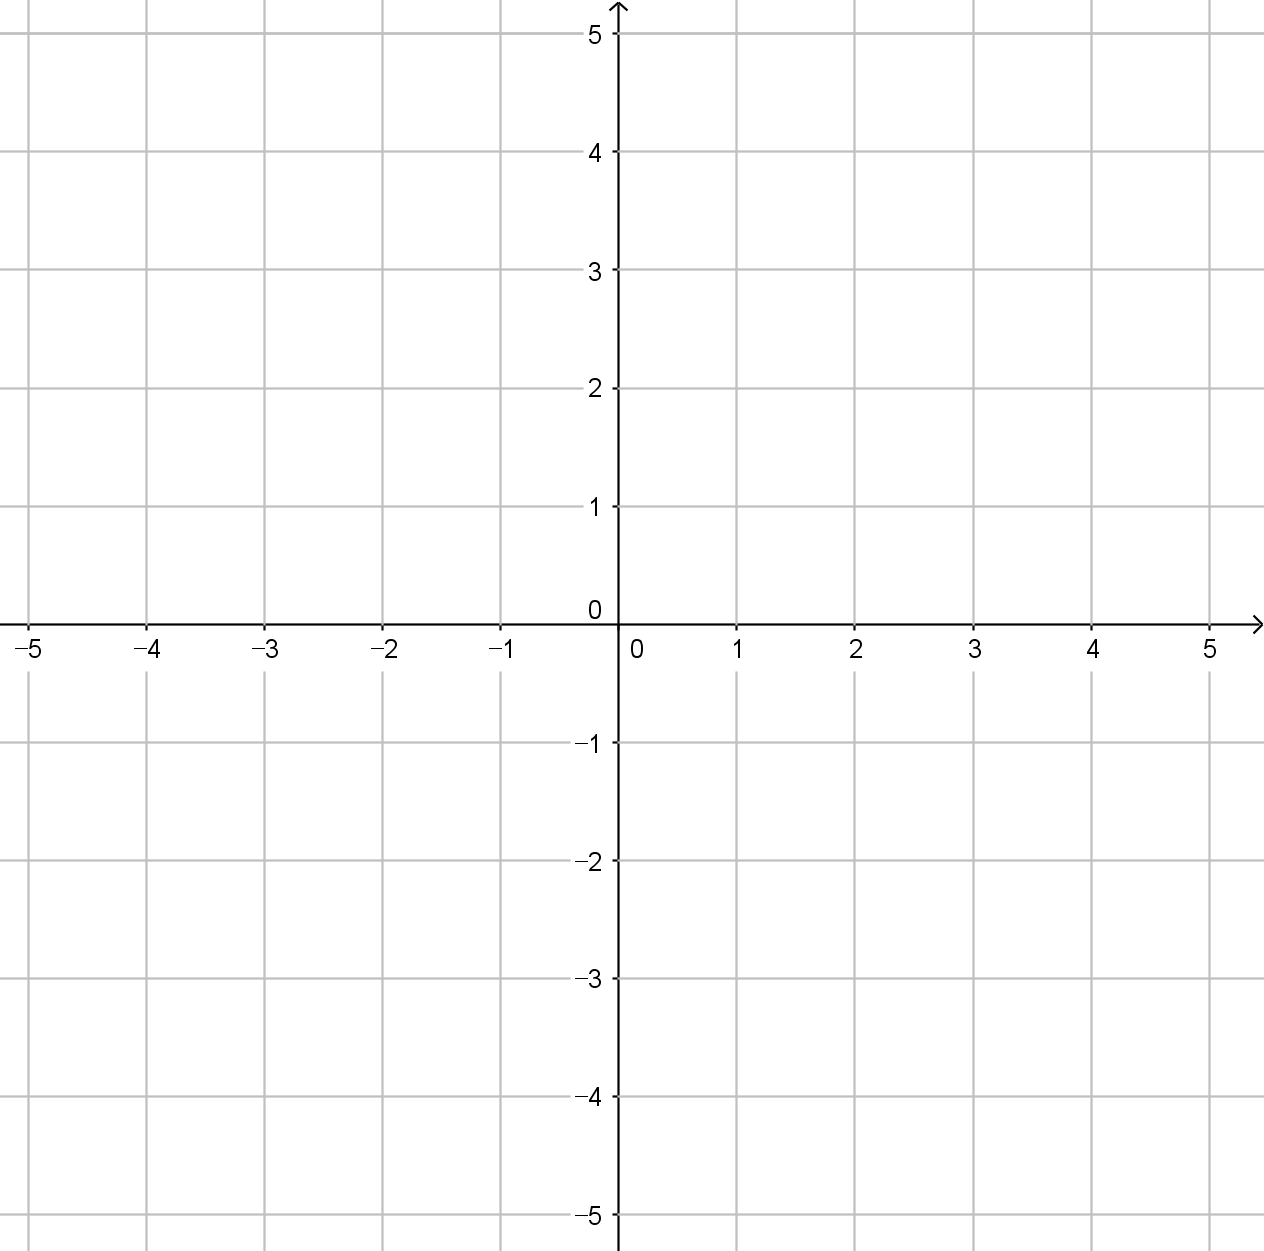
\includegraphics[width=0.9\textwidth]{55}
\end{minipage}
\begin{minipage}{0.45\textwidth}\centering
\(y=-2x^2\)
\par\bigskip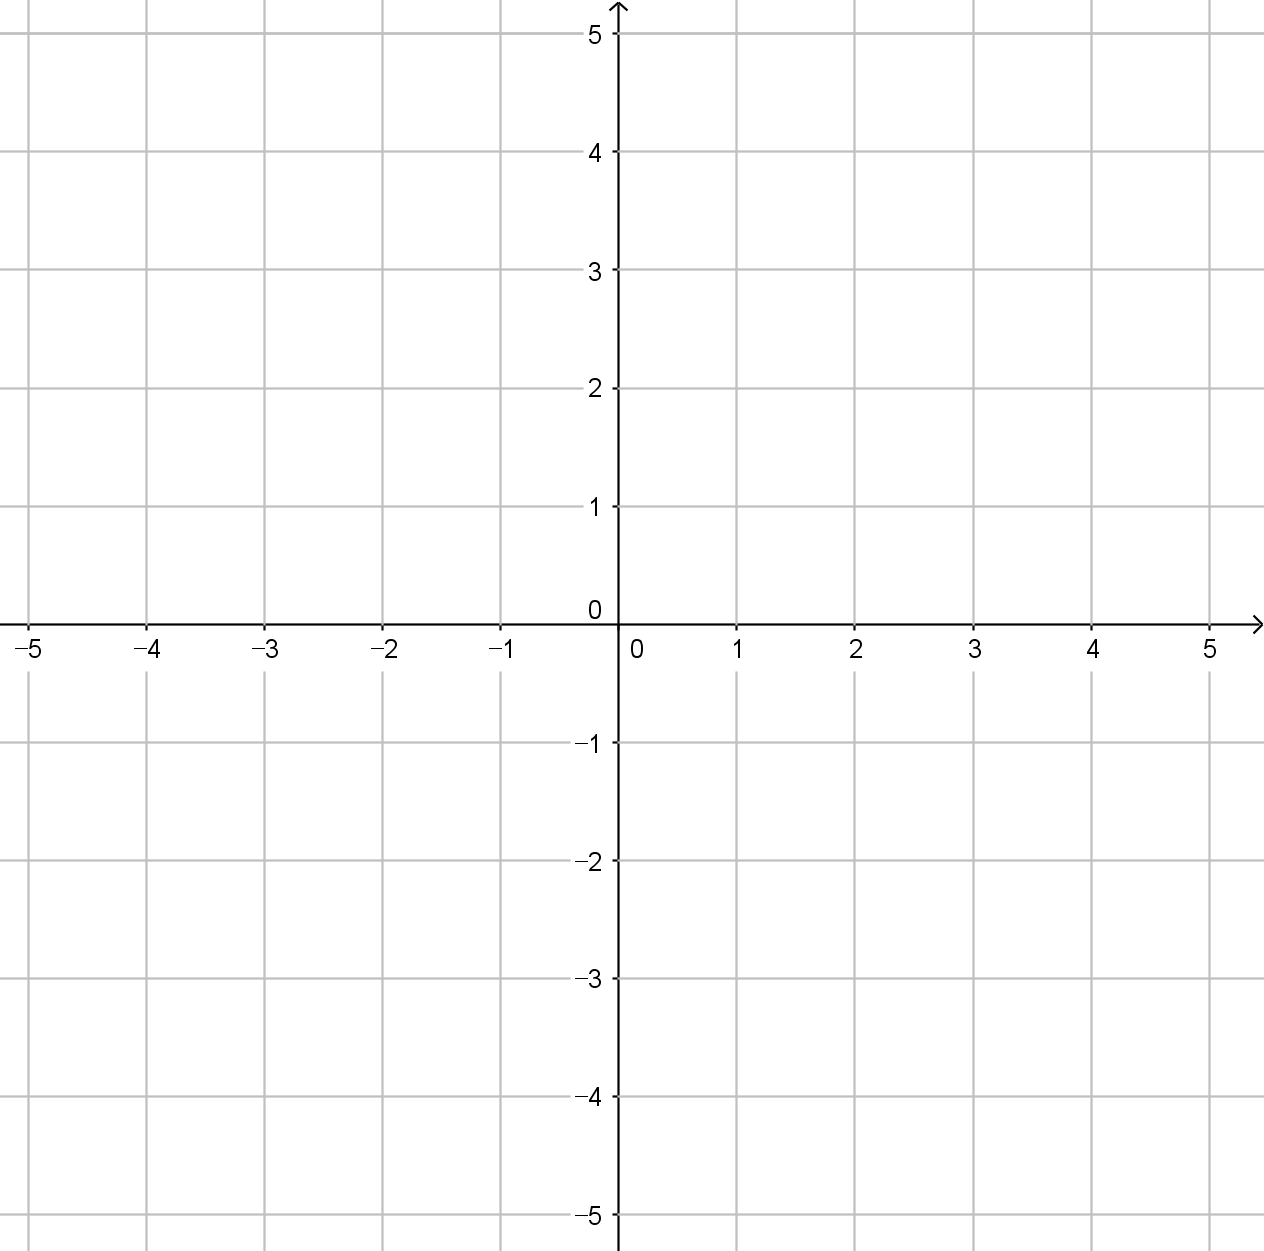
\includegraphics[width=0.9\textwidth]{55}
\end{minipage}\bigskip\bigskip\par


\clearpage
\begin{minipage}{0.45\textwidth}\centering
\(y=3x^2\)
\par\bigskip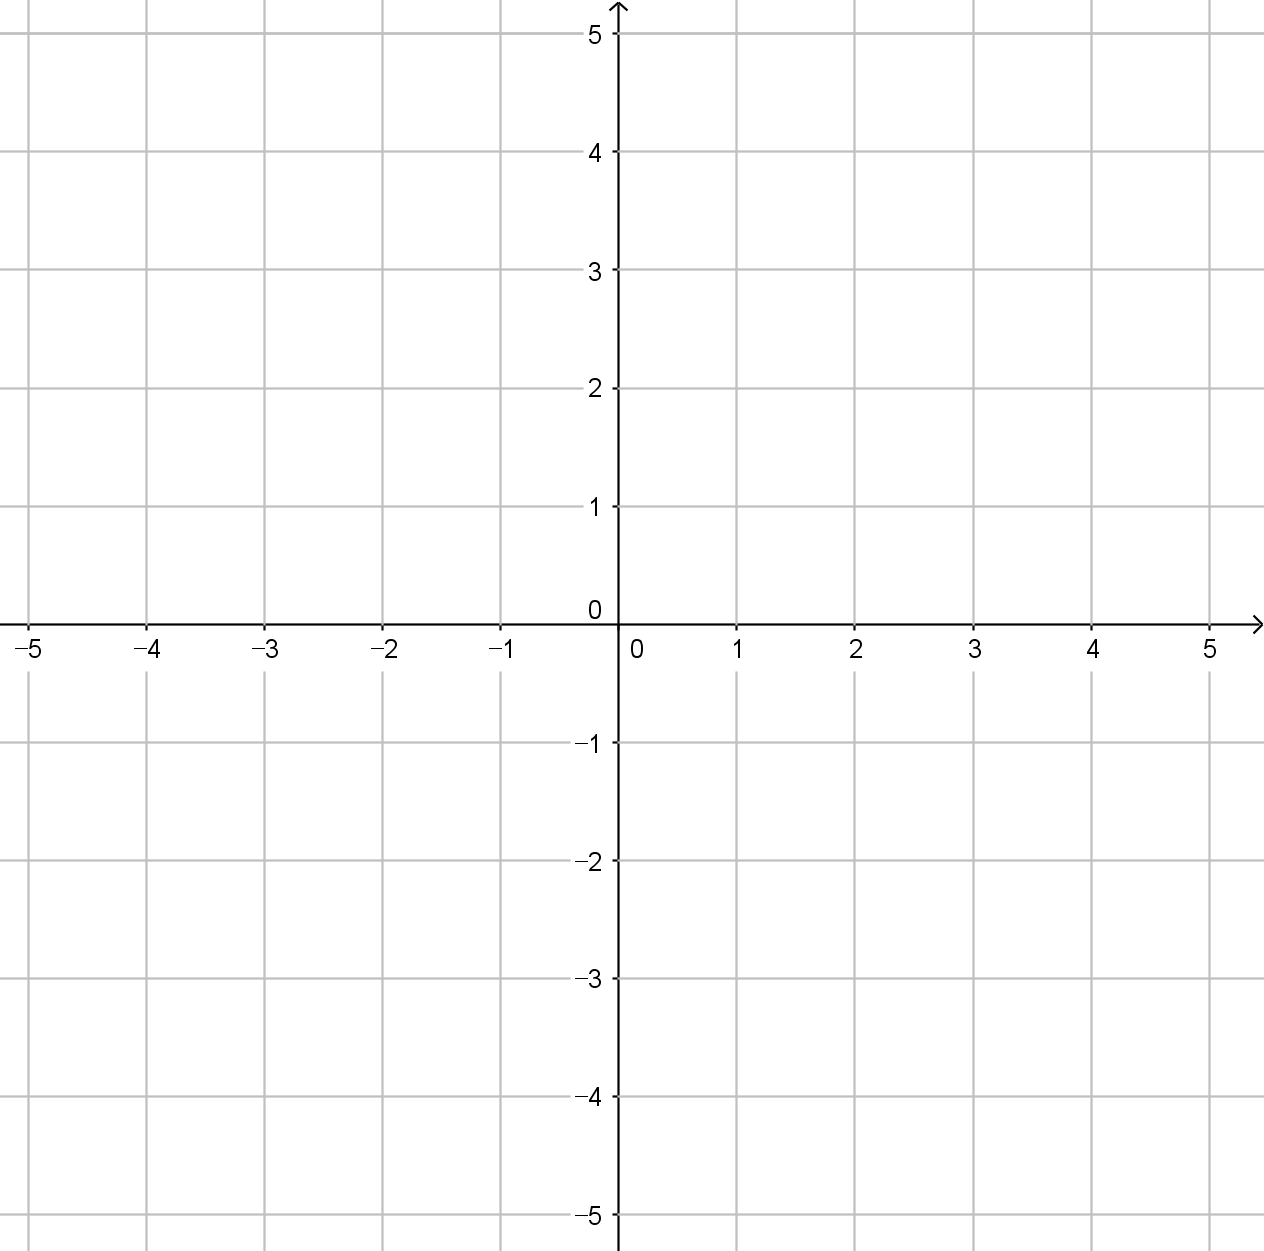
\includegraphics[width=0.9\textwidth]{55}
\end{minipage}
\begin{minipage}{0.45\textwidth}\centering
\(y=-3x^2\)
\par\bigskip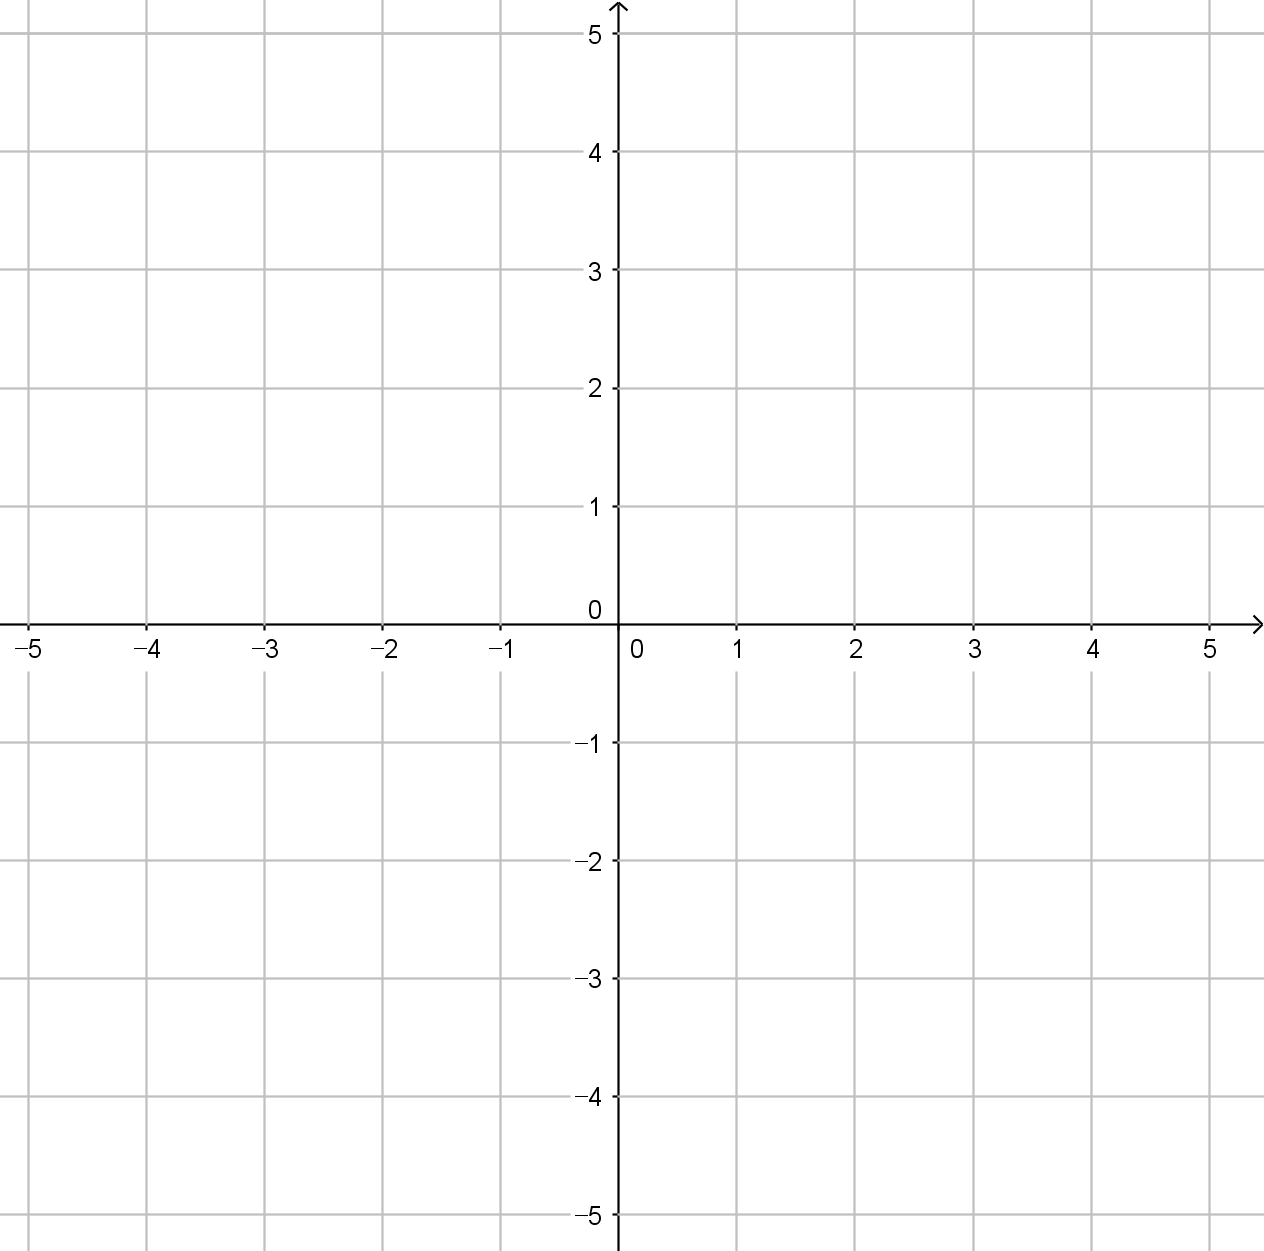
\includegraphics[width=0.9\textwidth]{55}
\end{minipage}\bigskip\bigskip\par
\begin{minipage}{0.45\textwidth}\centering
\(y=\frac12x^2\)
\par\bigskip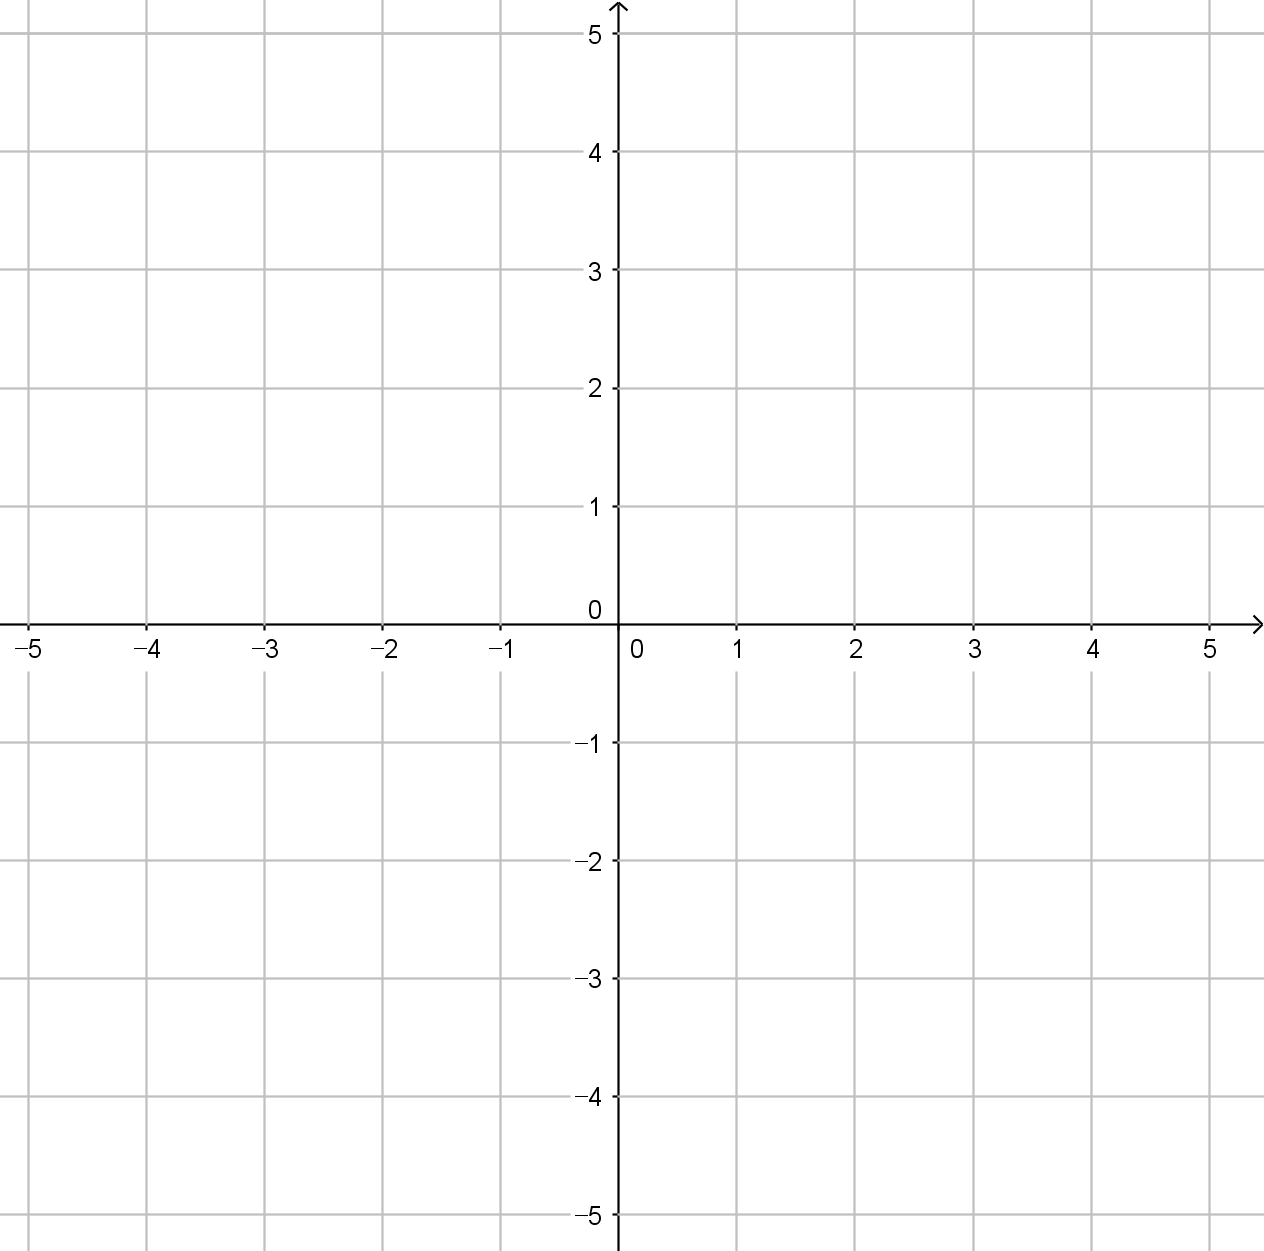
\includegraphics[width=0.9\textwidth]{55}
\end{minipage}
\begin{minipage}{0.45\textwidth}\centering
\(y=-\frac12x^2\)
\par\bigskip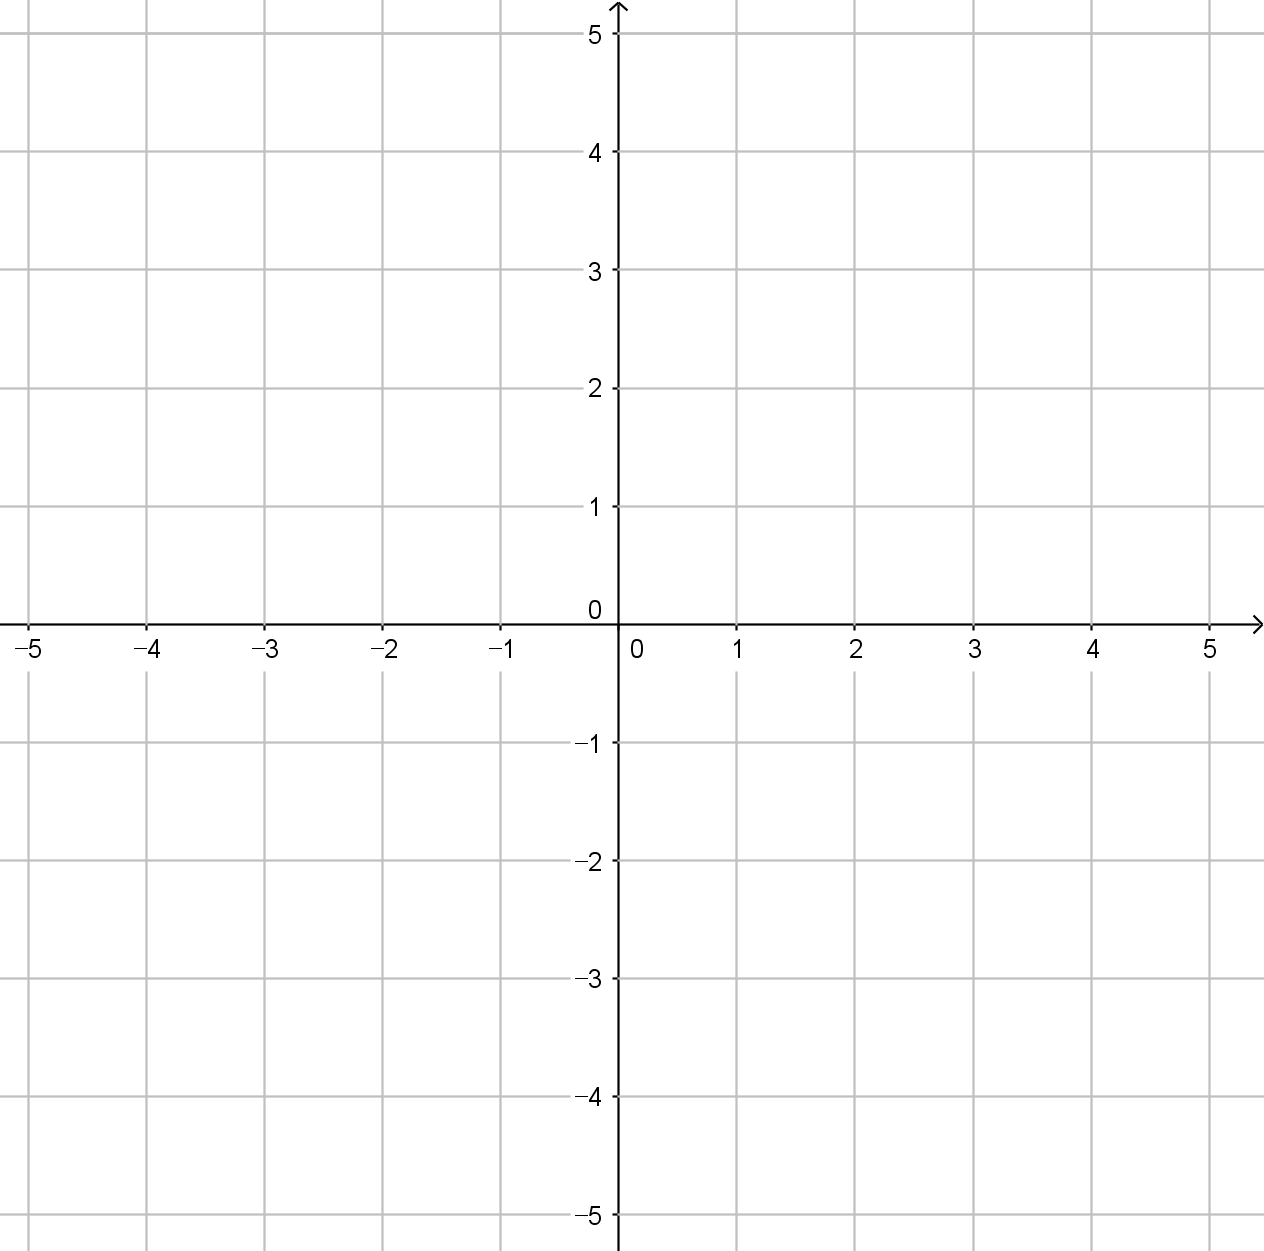
\includegraphics[width=0.9\textwidth]{55}
\end{minipage}\bigskip\bigskip\par
\begin{minipage}{0.45\textwidth}\centering
\(y=x^2+1\)
\par\bigskip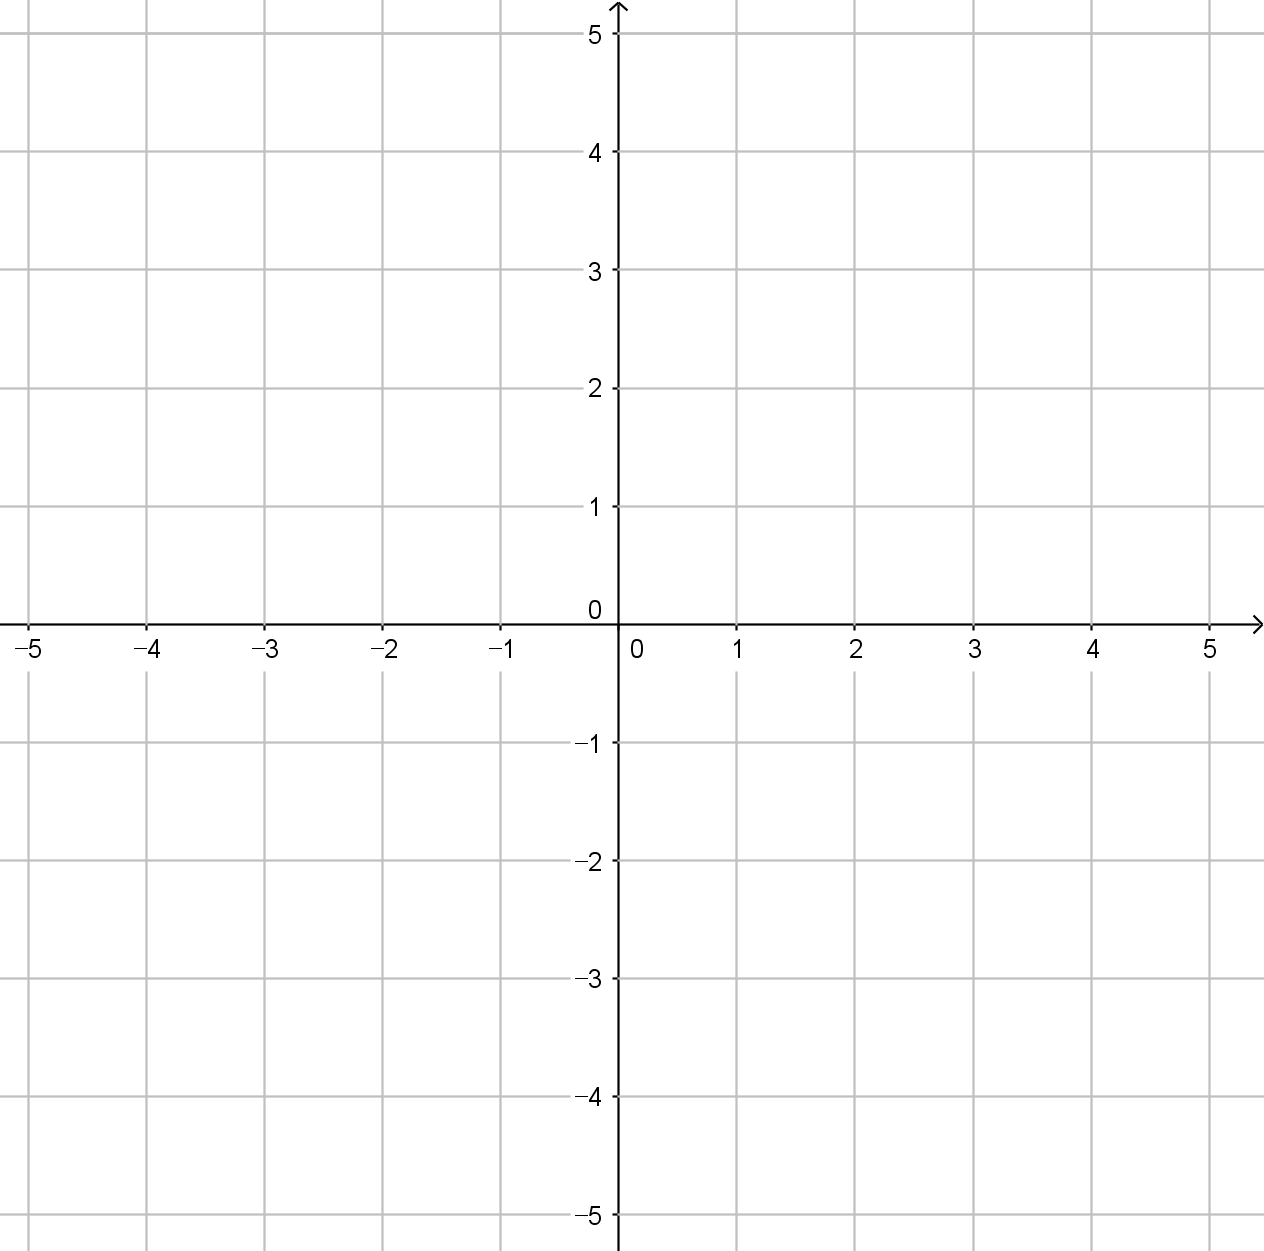
\includegraphics[width=0.9\textwidth]{55}
\end{minipage}
\begin{minipage}{0.45\textwidth}\centering
\(y=x^2-2\)
\par\bigskip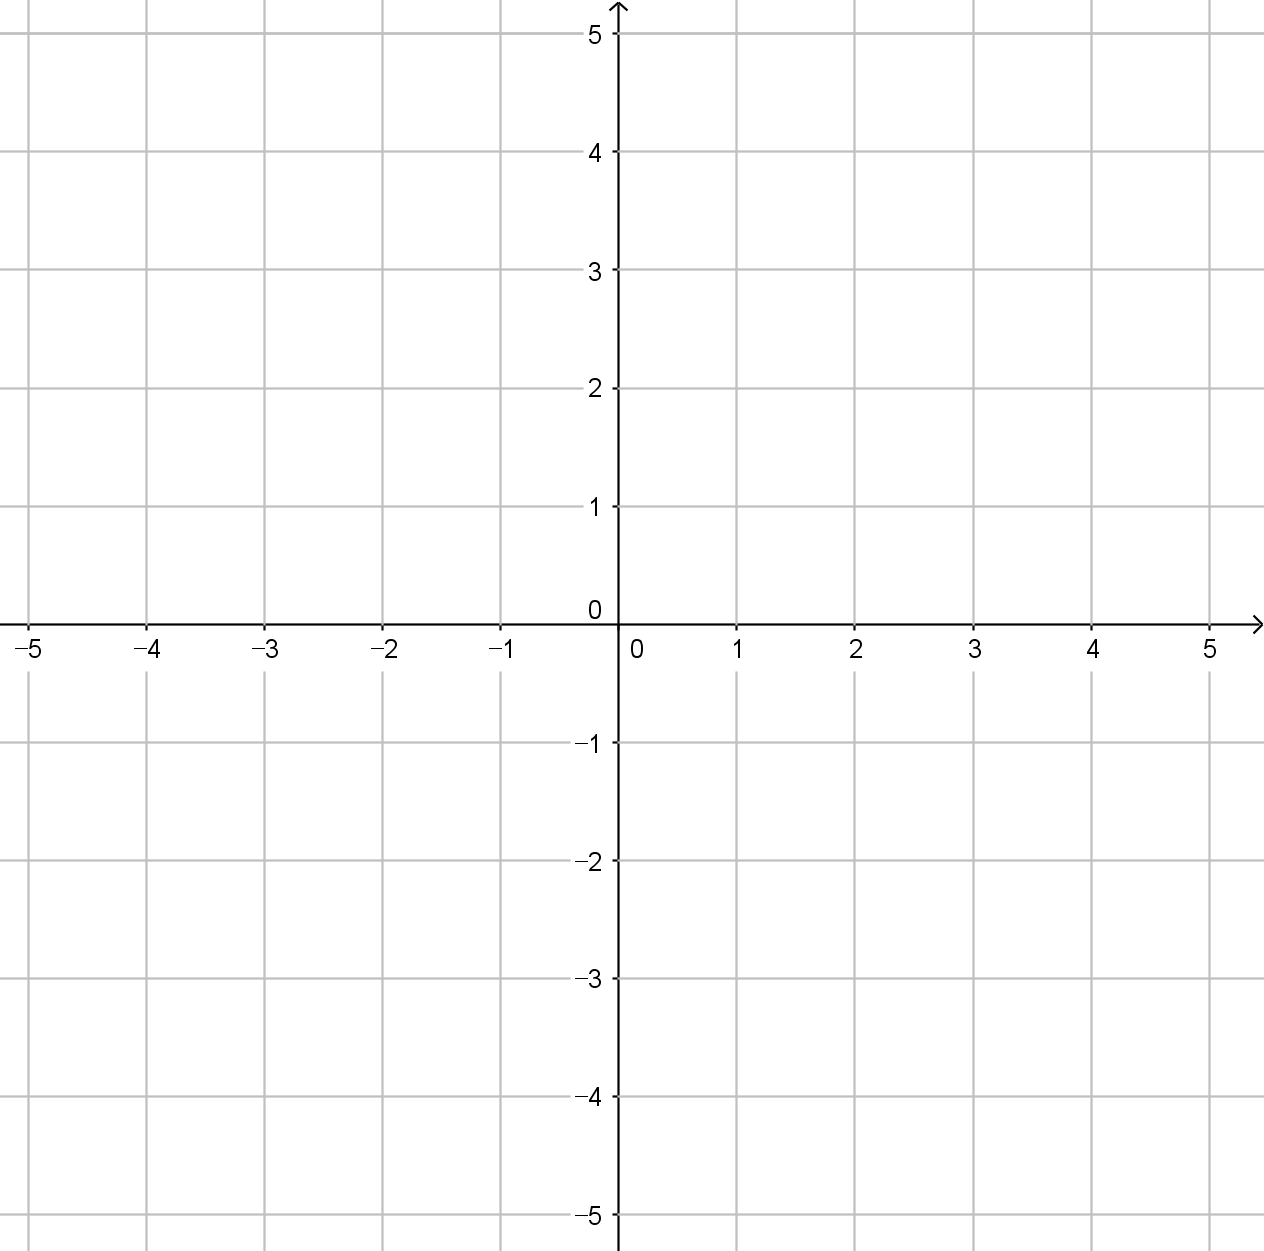
\includegraphics[width=0.9\textwidth]{55}
\end{minipage}\bigskip\bigskip\par


\clearpage
\begin{minipage}{0.45\textwidth}\centering
\(y=-x^2+3\)
\par\bigskip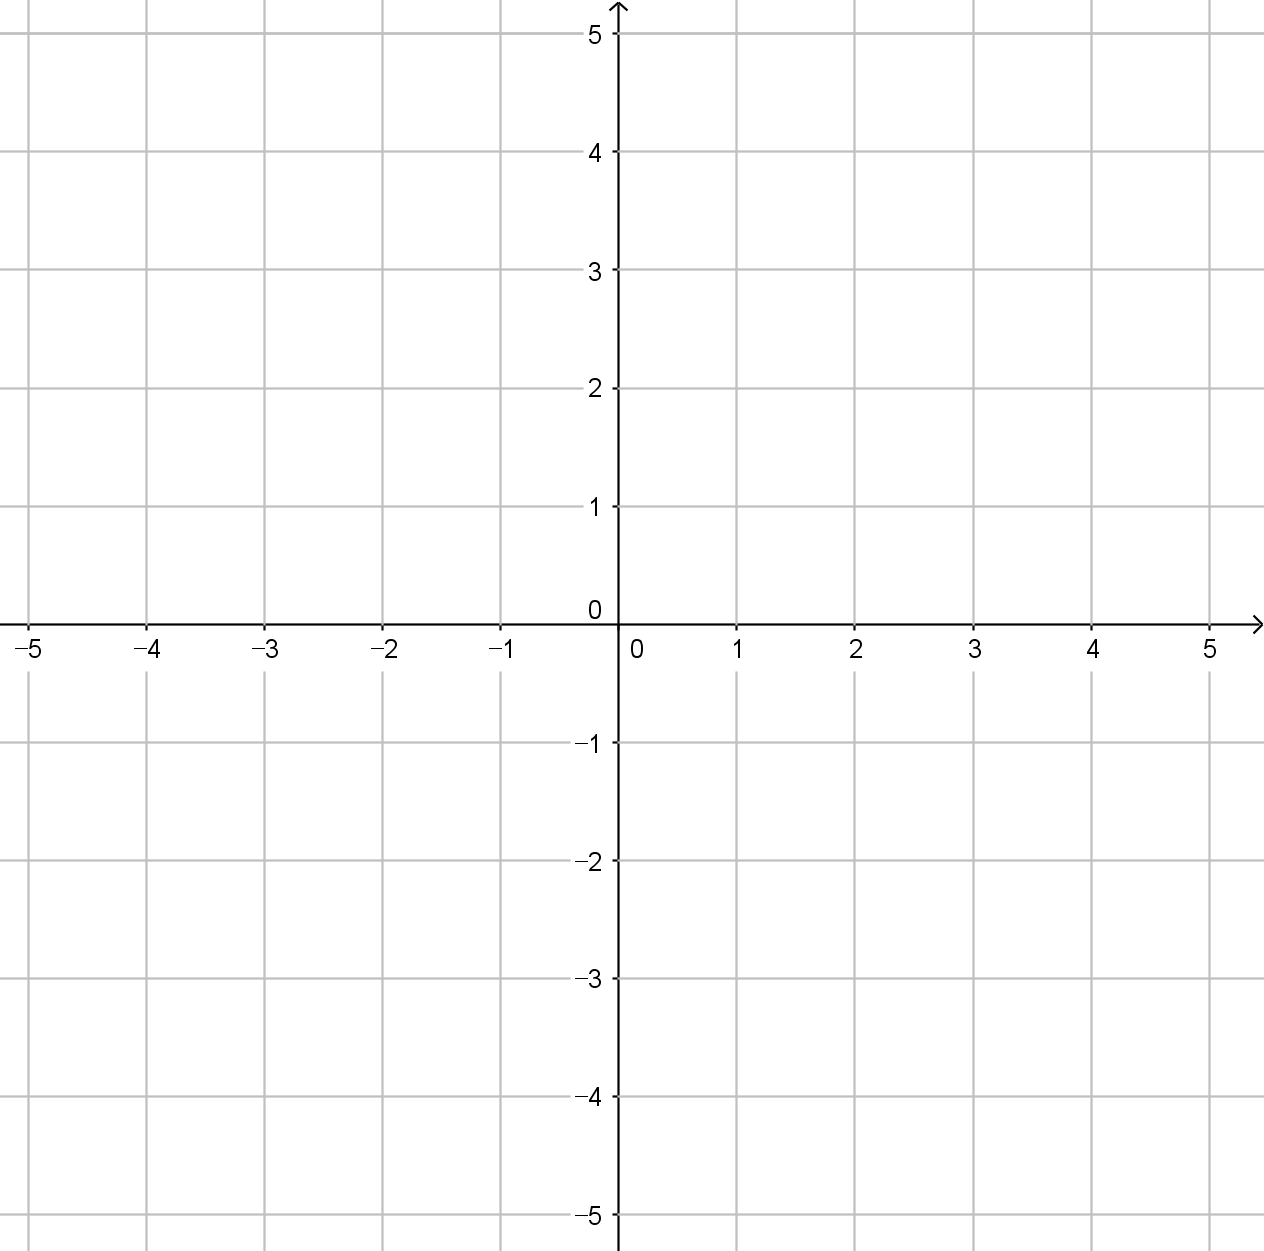
\includegraphics[width=0.9\textwidth]{55}
\end{minipage}
\begin{minipage}{0.45\textwidth}\centering
\(y=4-x^2\)
\par\bigskip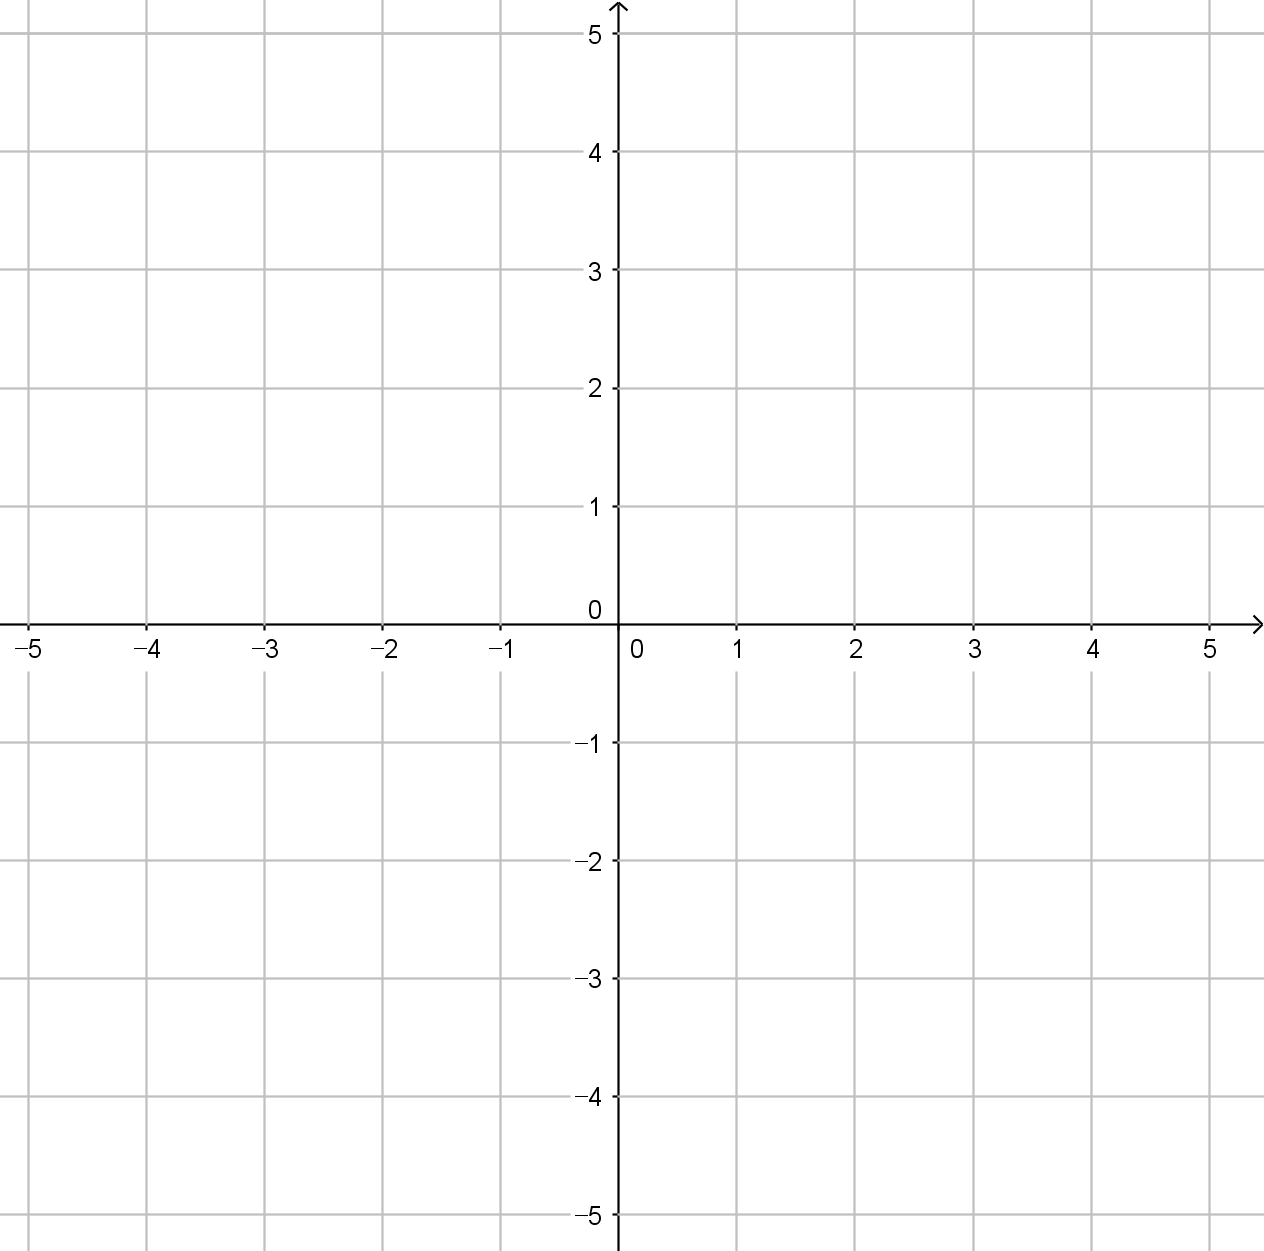
\includegraphics[width=0.9\textwidth]{55}
\end{minipage}\bigskip\bigskip\par
\begin{minipage}{0.45\textwidth}\centering
\(y=2x^2-4\)
\par\bigskip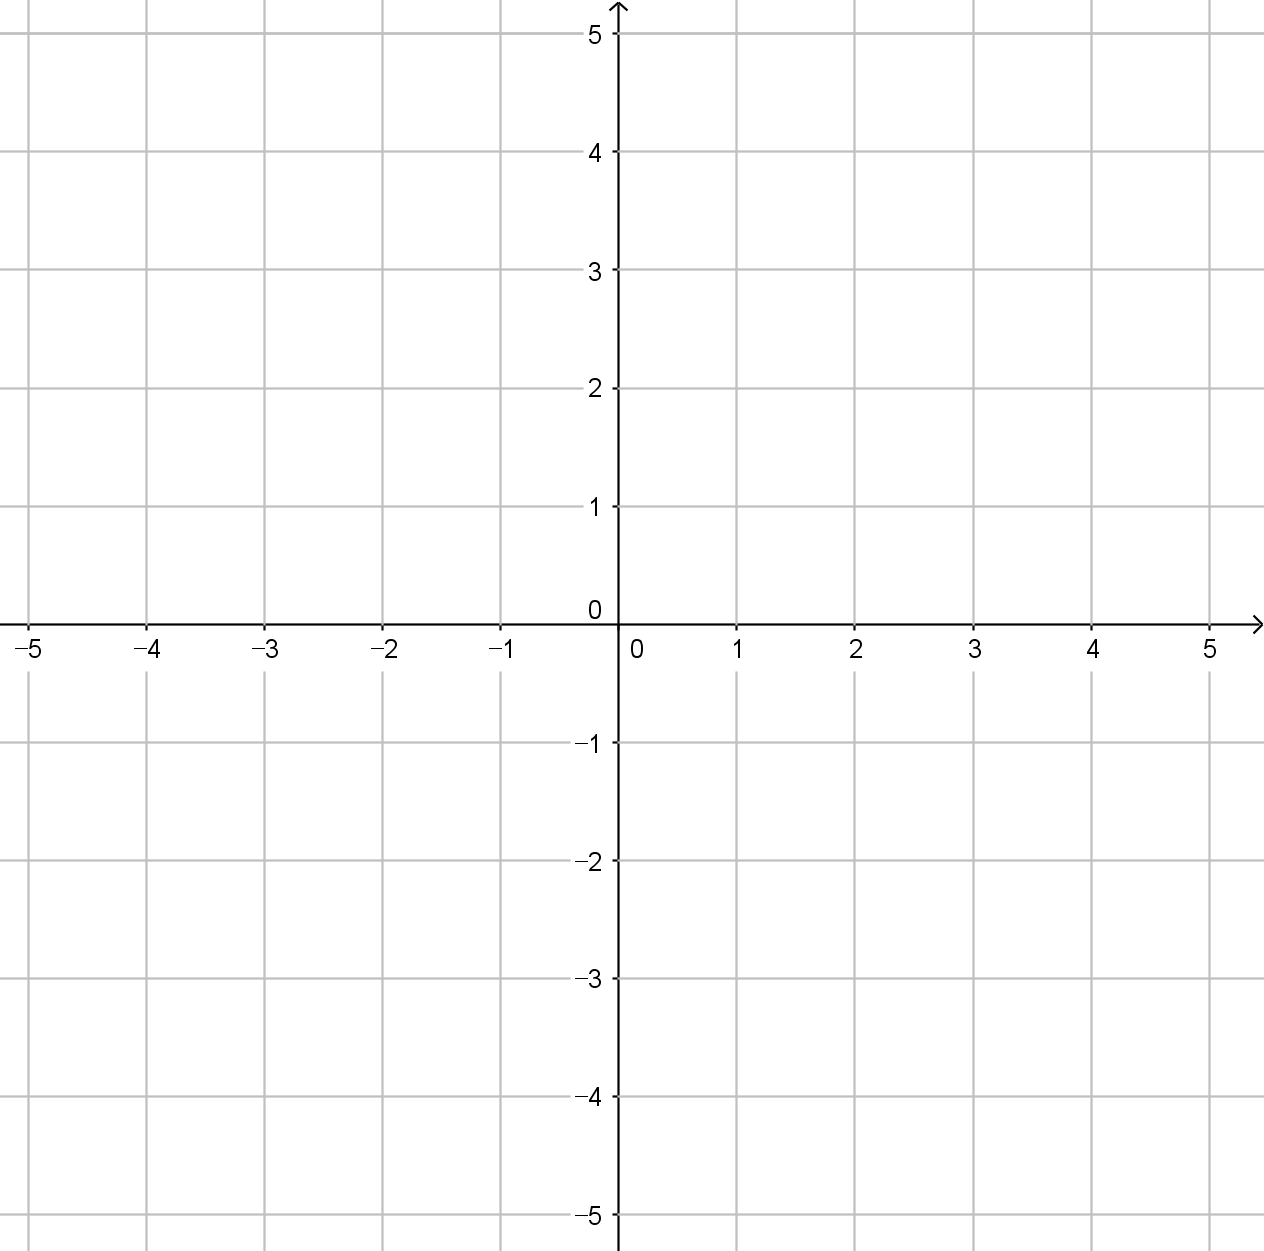
\includegraphics[width=0.9\textwidth]{55}
\end{minipage}
\begin{minipage}{0.45\textwidth}\centering
\(y=(x-1)^2\)
\par\bigskip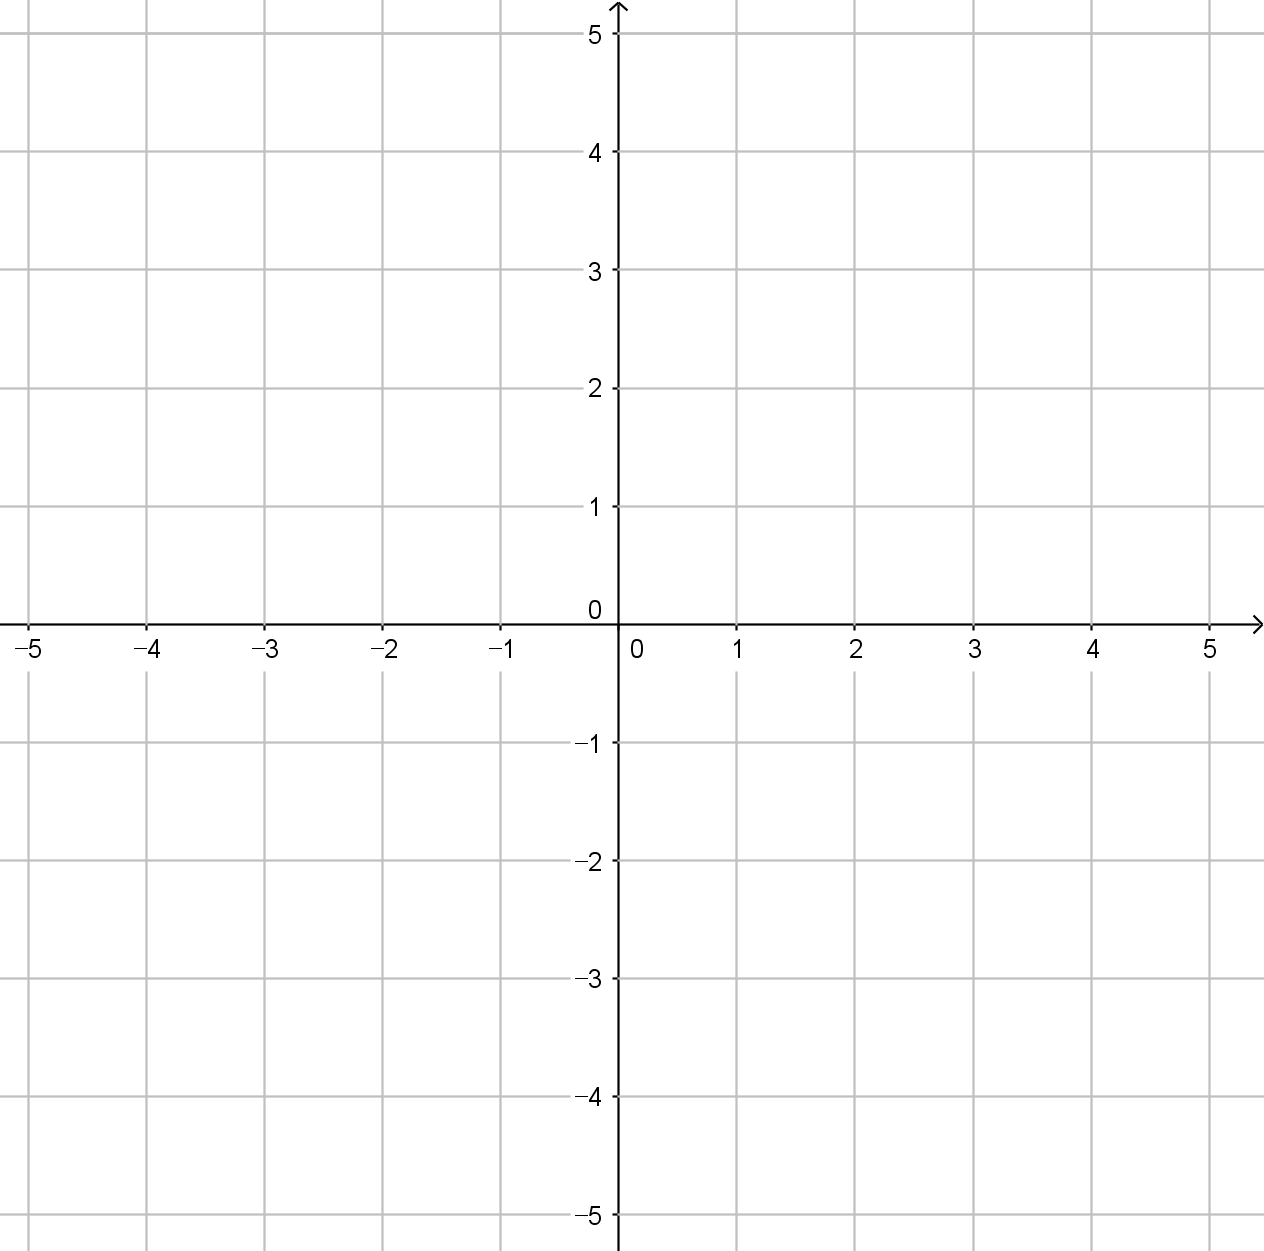
\includegraphics[width=0.9\textwidth]{55}
\end{minipage}\bigskip\bigskip\par
\begin{minipage}{0.45\textwidth}\centering
\(y=(x+2)^2\)
\par\bigskip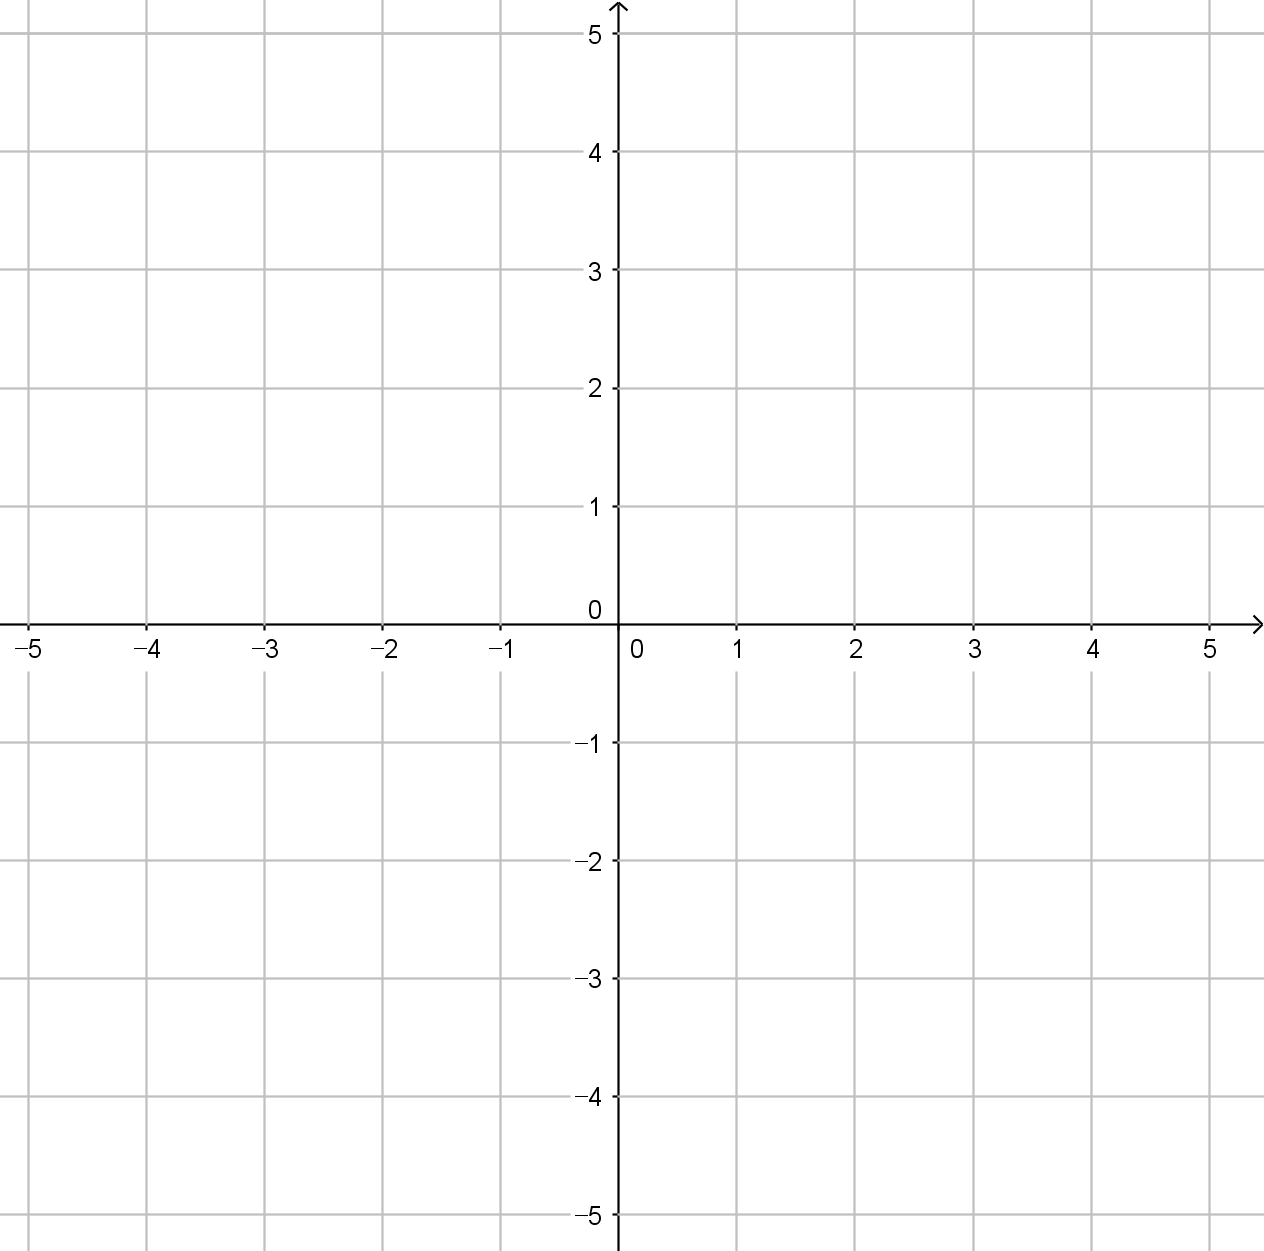
\includegraphics[width=0.9\textwidth]{55}
\end{minipage}
\begin{minipage}{0.45\textwidth}\centering
\(y=2(x-2)^2\)
\par\bigskip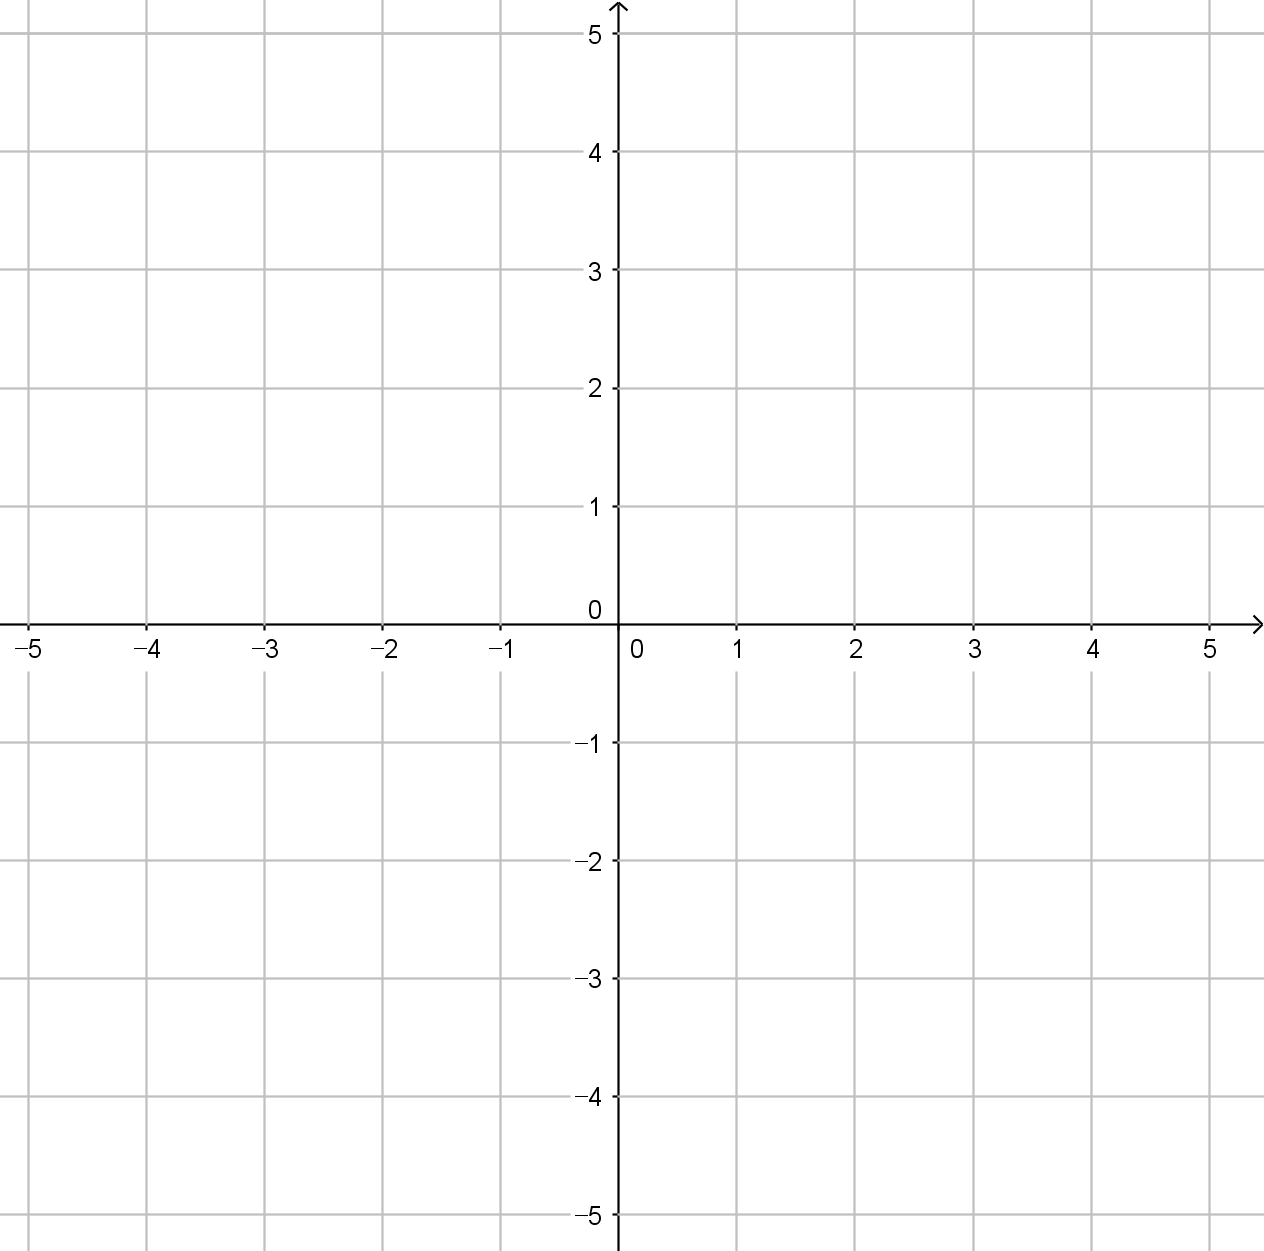
\includegraphics[width=0.9\textwidth]{55}
\end{minipage}\bigskip\bigskip\par

\clearpage
\begin{minipage}{0.45\textwidth}\centering
\(y=(x-1)^2+2\)
\par\bigskip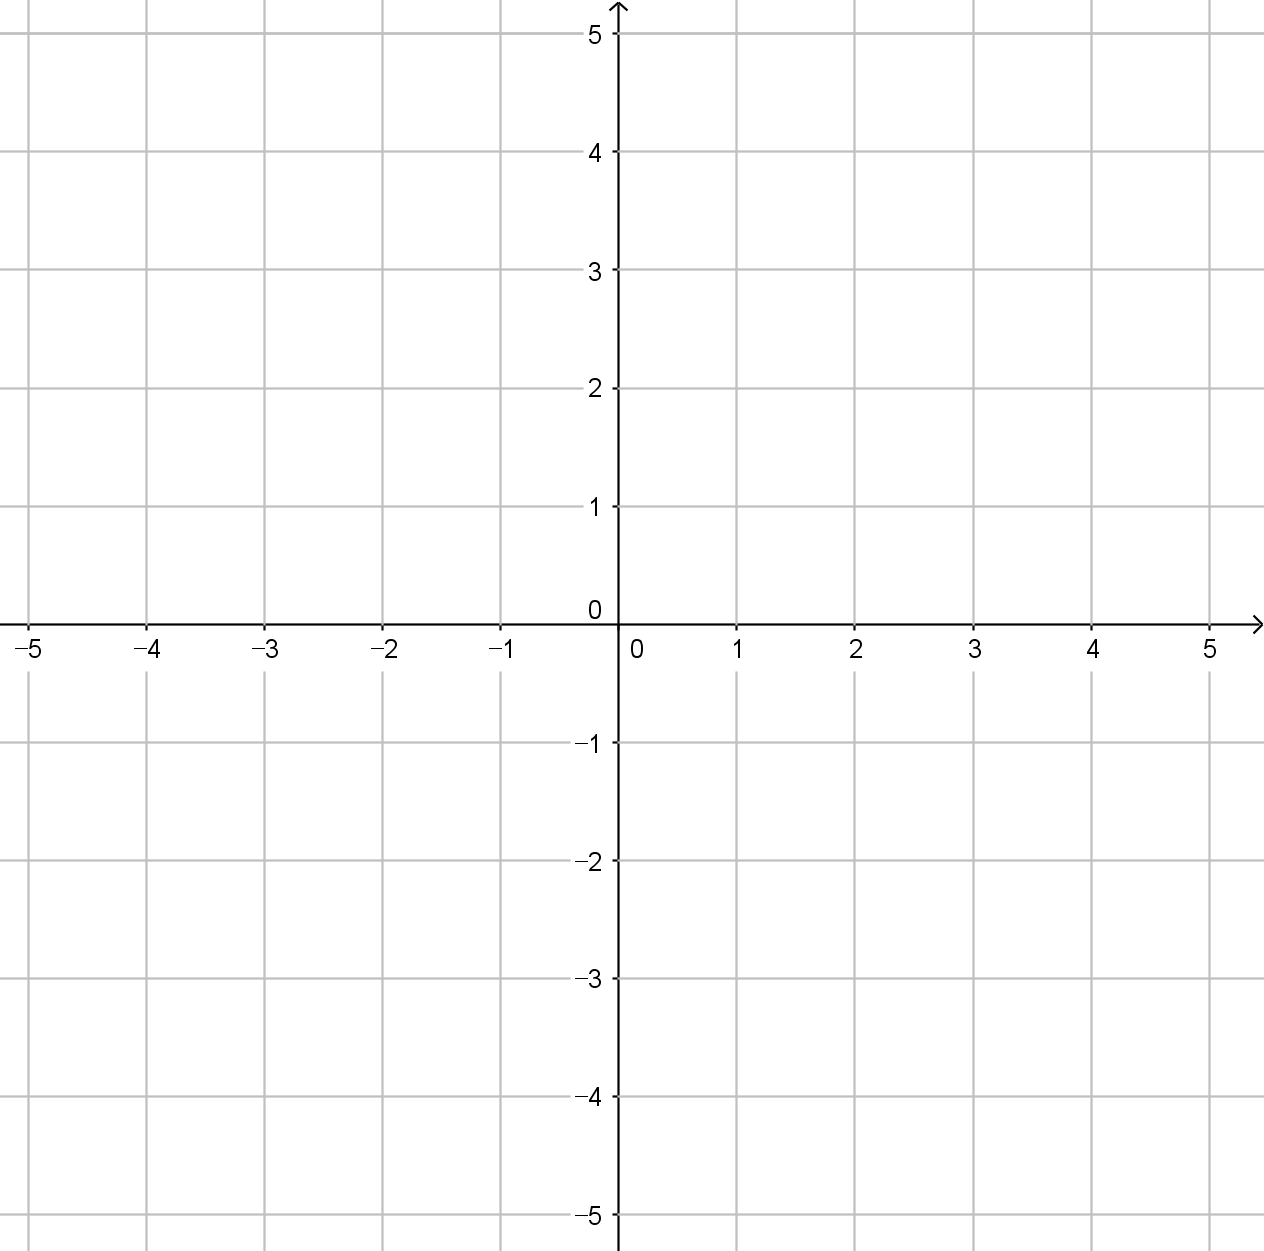
\includegraphics[width=0.9\textwidth]{55}
\end{minipage}
\begin{minipage}{0.45\textwidth}\centering
\(y=2(x+3)^2-1\)
\par\bigskip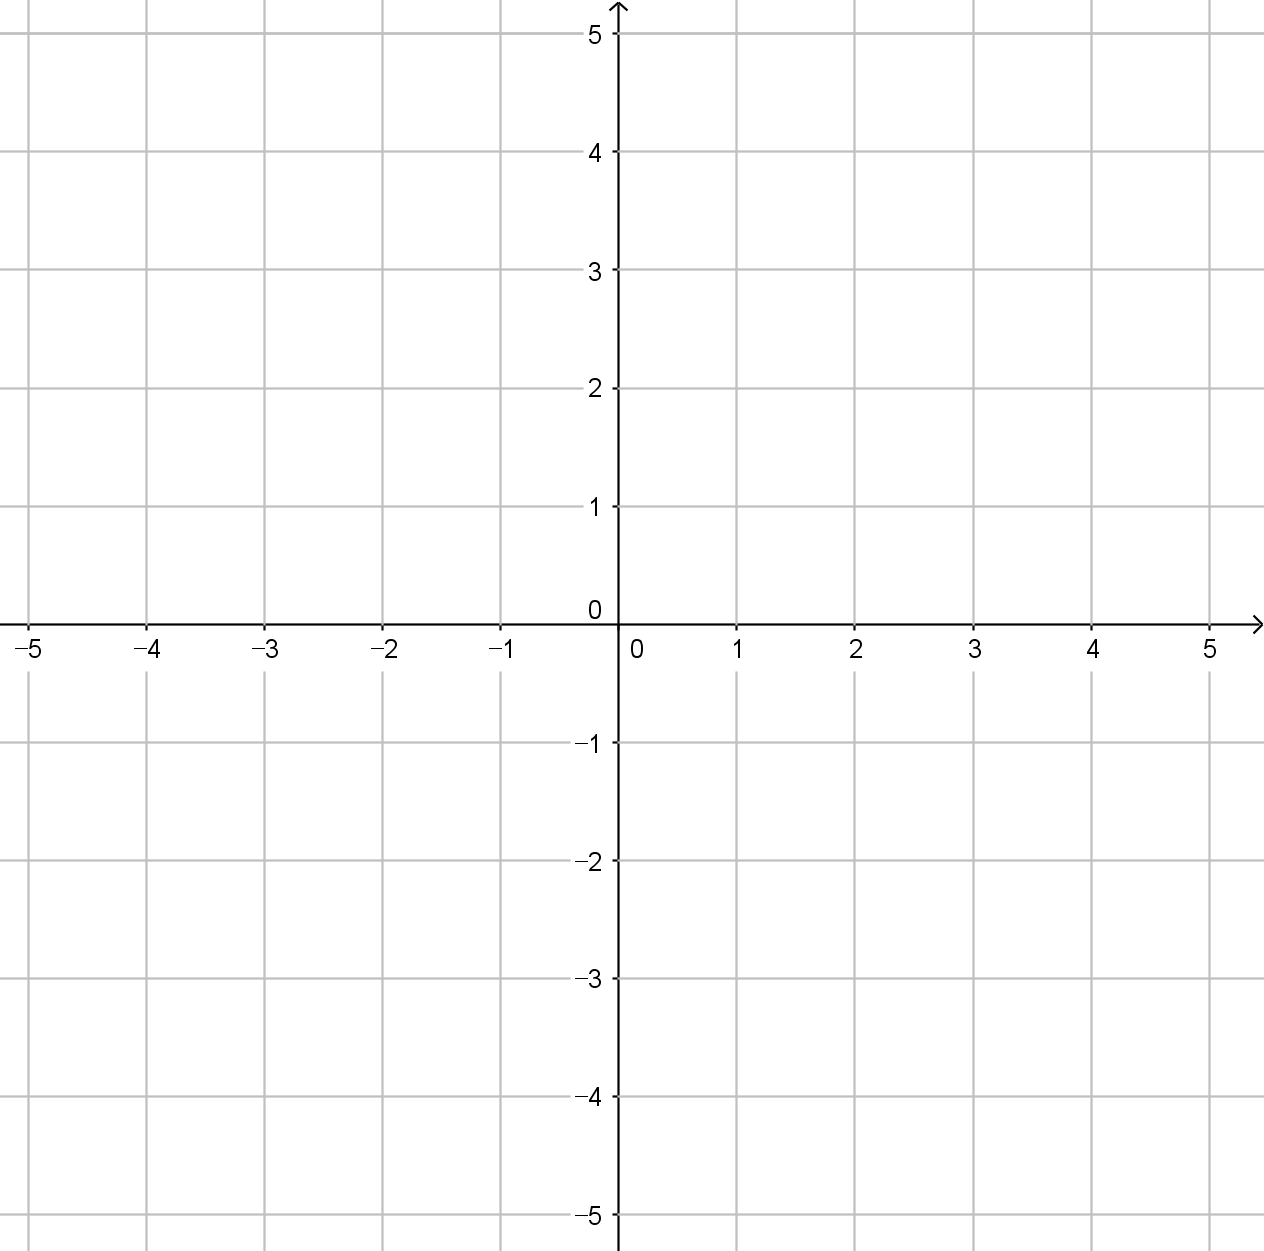
\includegraphics[width=0.9\textwidth]{55}
\end{minipage}\bigskip\bigskip\par
\begin{minipage}{0.45\textwidth}\centering
\(y=-(x-2)^2+4\)
\par\bigskip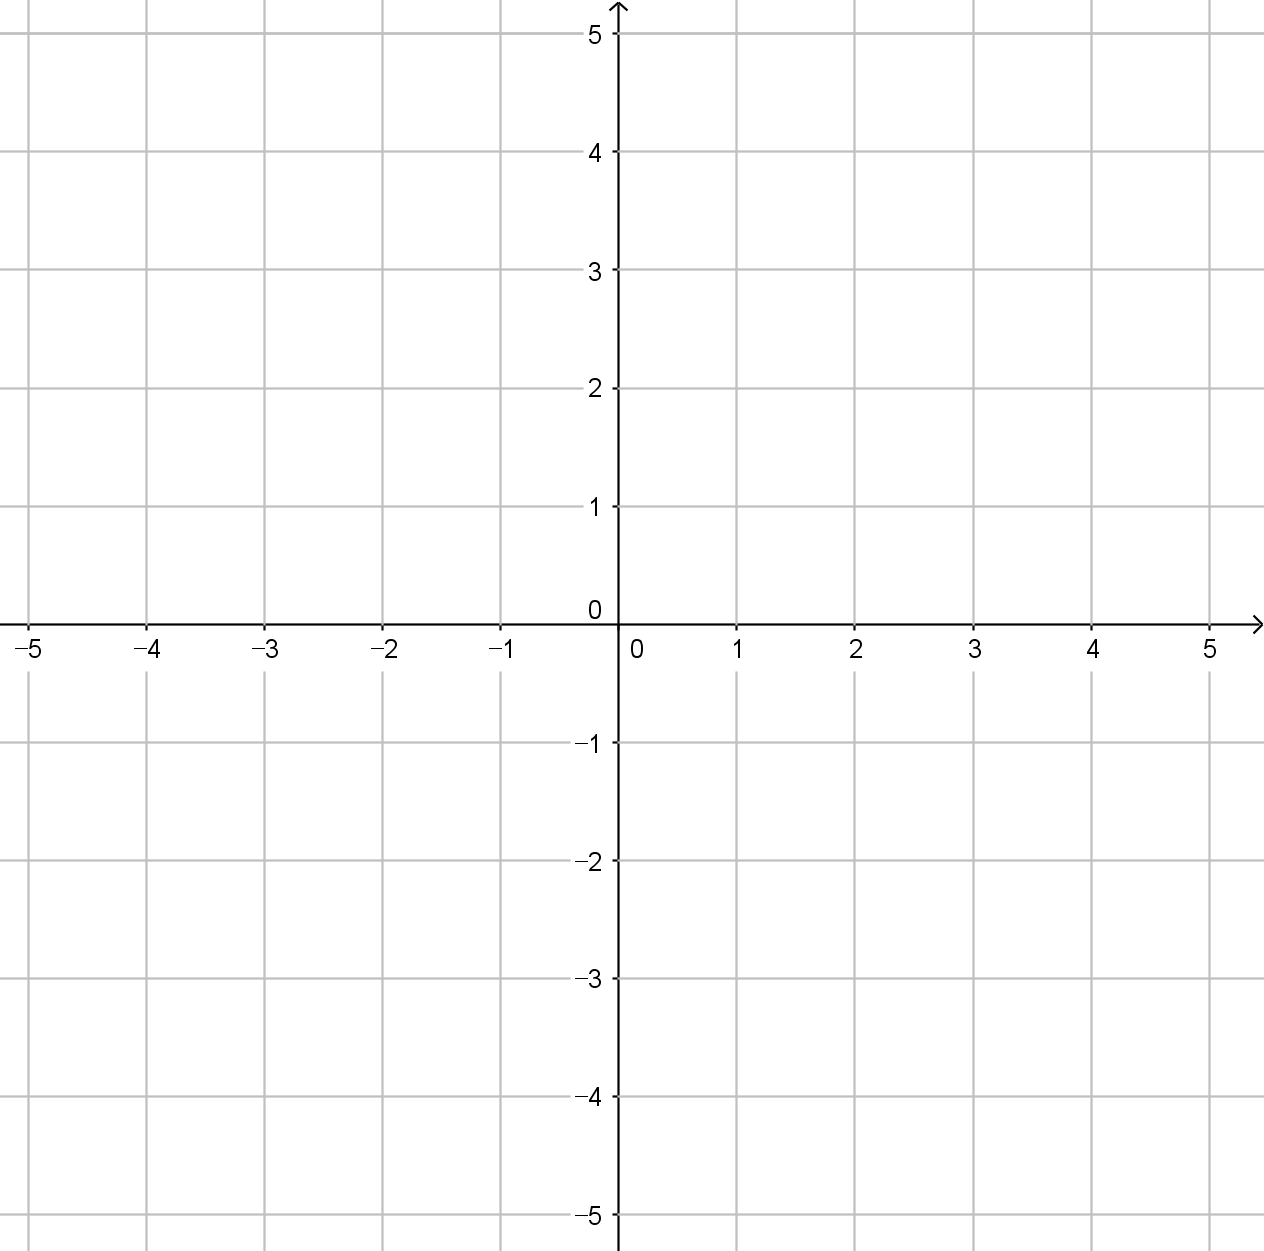
\includegraphics[width=0.9\textwidth]{55}
\end{minipage}
\begin{minipage}{0.45\textwidth}\centering
\(y=\frac12(x+2)^2+1\)
\par\bigskip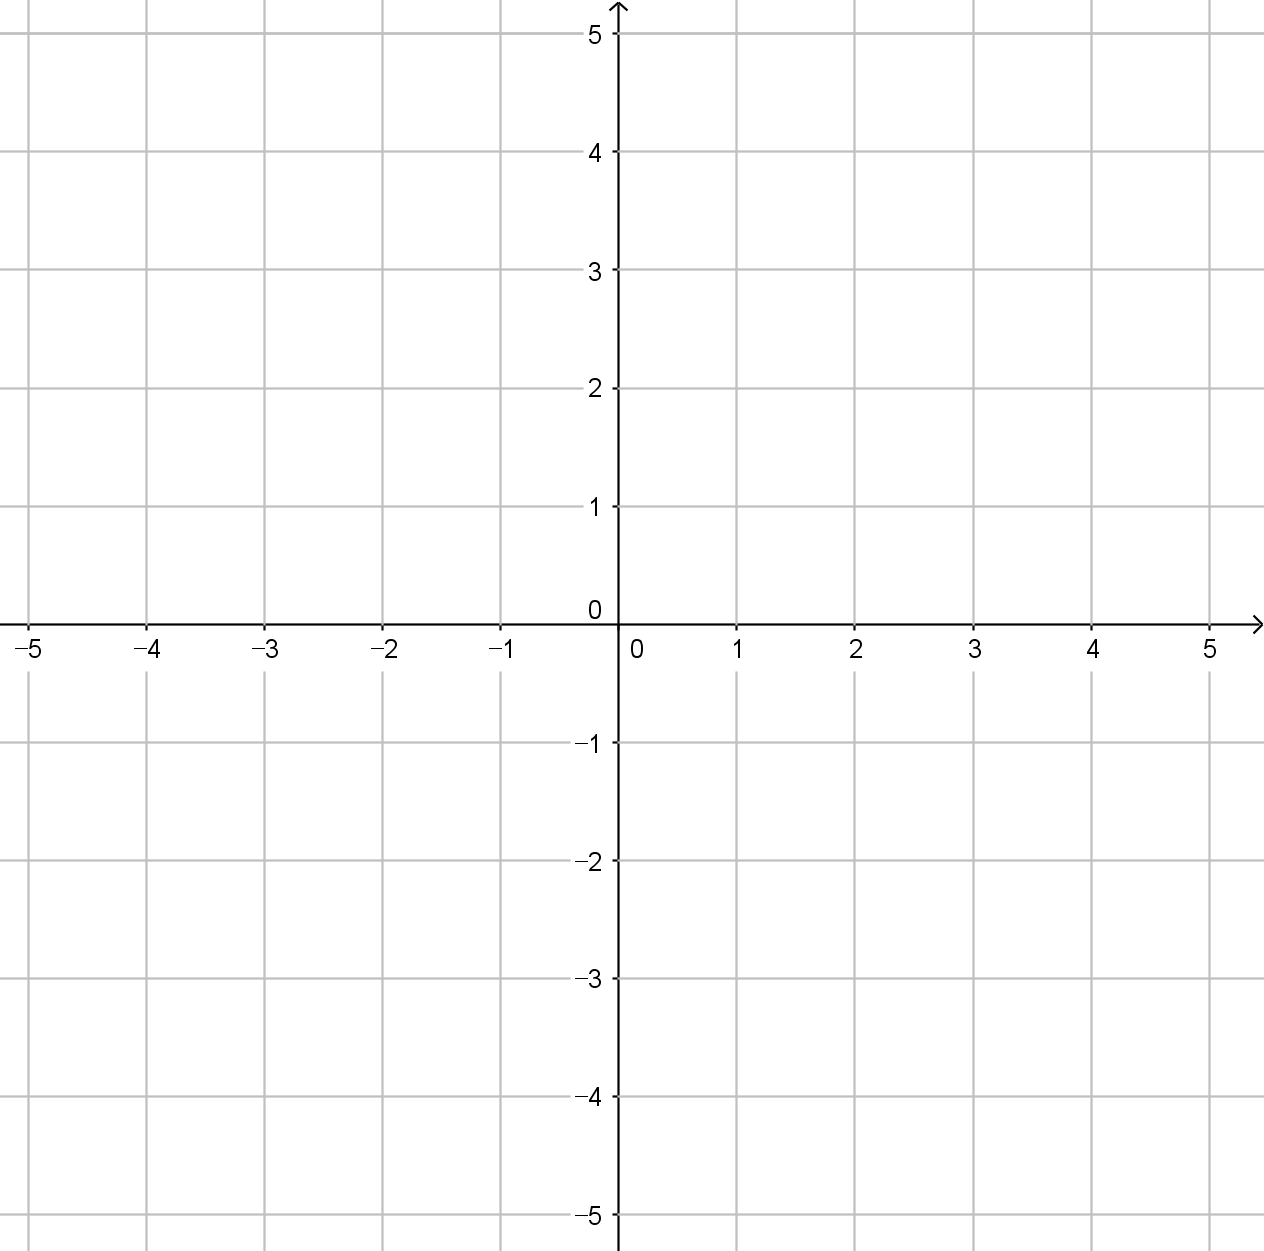
\includegraphics[width=0.9\textwidth]{55}
\end{minipage}\bigskip\bigskip\par

\clearpage
\begin{minipage}{0.45\textwidth}\centering
\(y=x^2+2x+1\)
\par\bigskip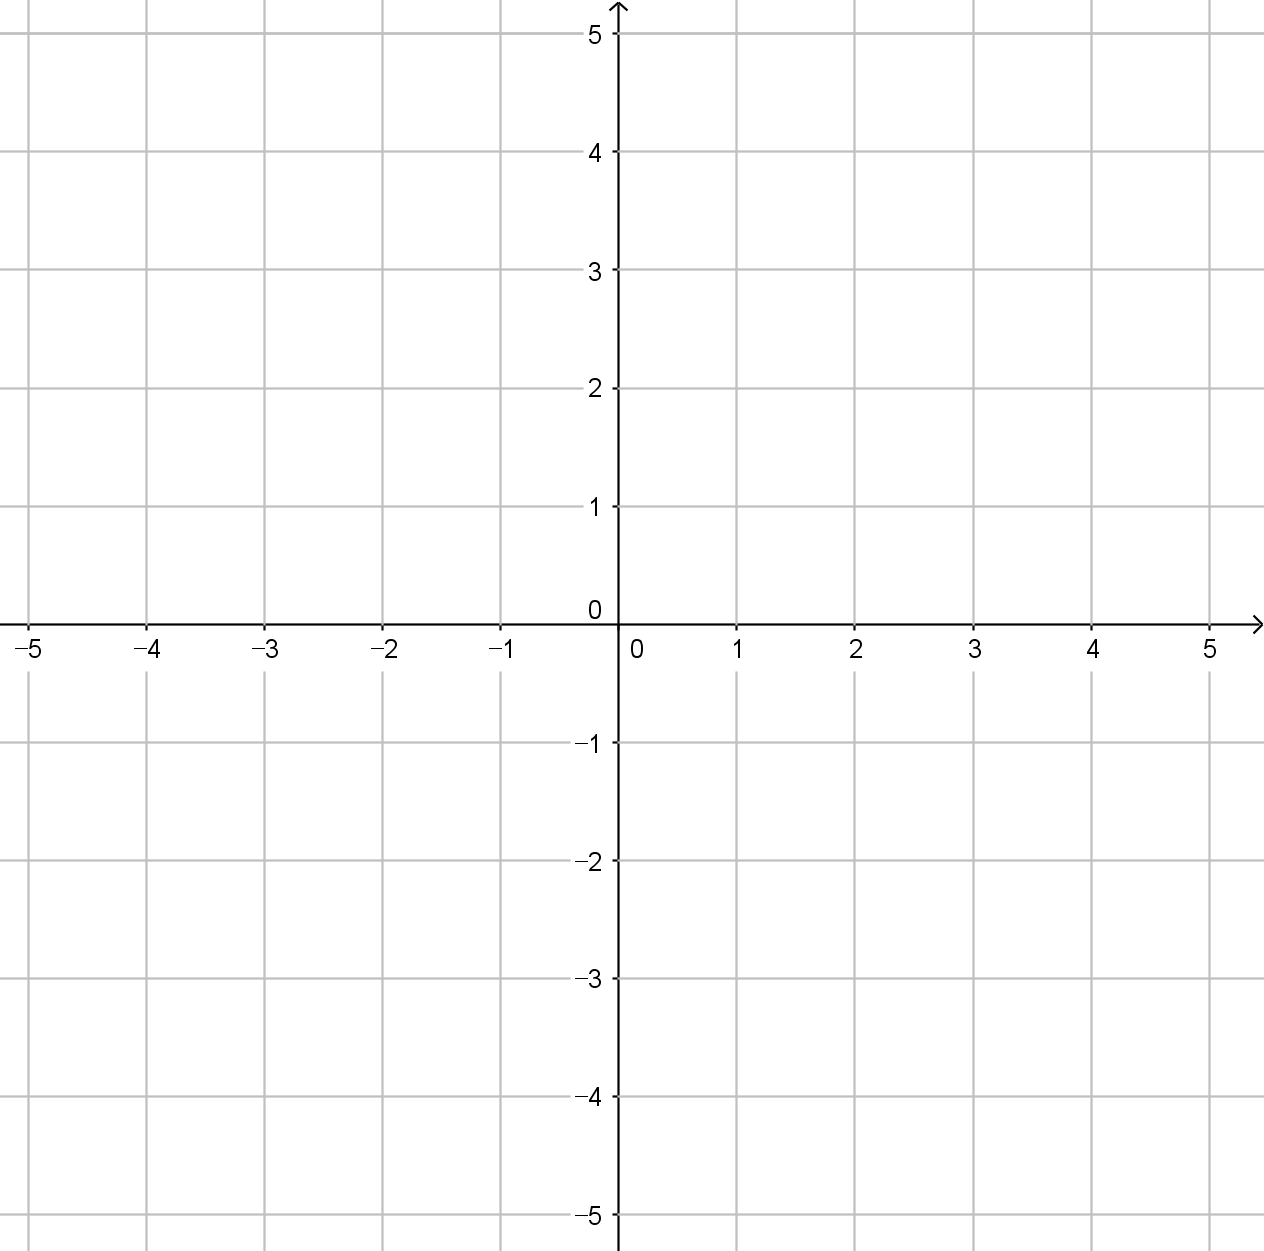
\includegraphics[width=0.9\textwidth]{55}
\end{minipage}
\begin{minipage}{0.45\textwidth}\centering
\(y=-x^2+4x-4\)
\par\bigskip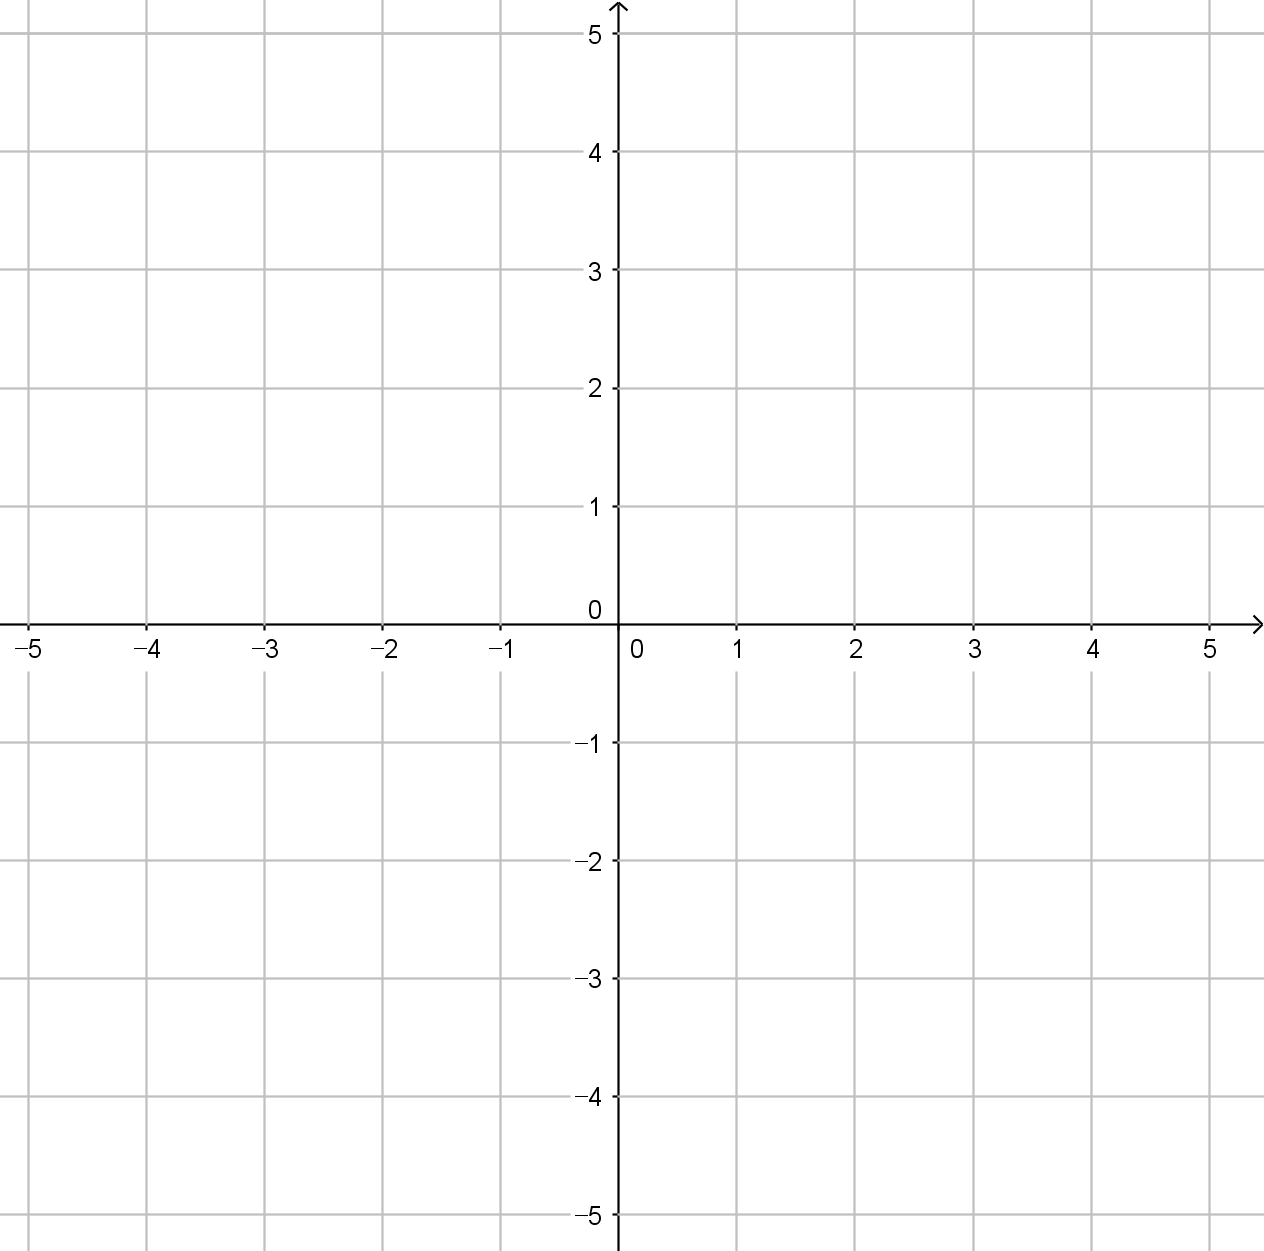
\includegraphics[width=0.9\textwidth]{55}
\end{minipage}\bigskip\bigskip\par
\begin{minipage}{0.45\textwidth}\centering
\(y=x^2-4x+2\)
\par\bigskip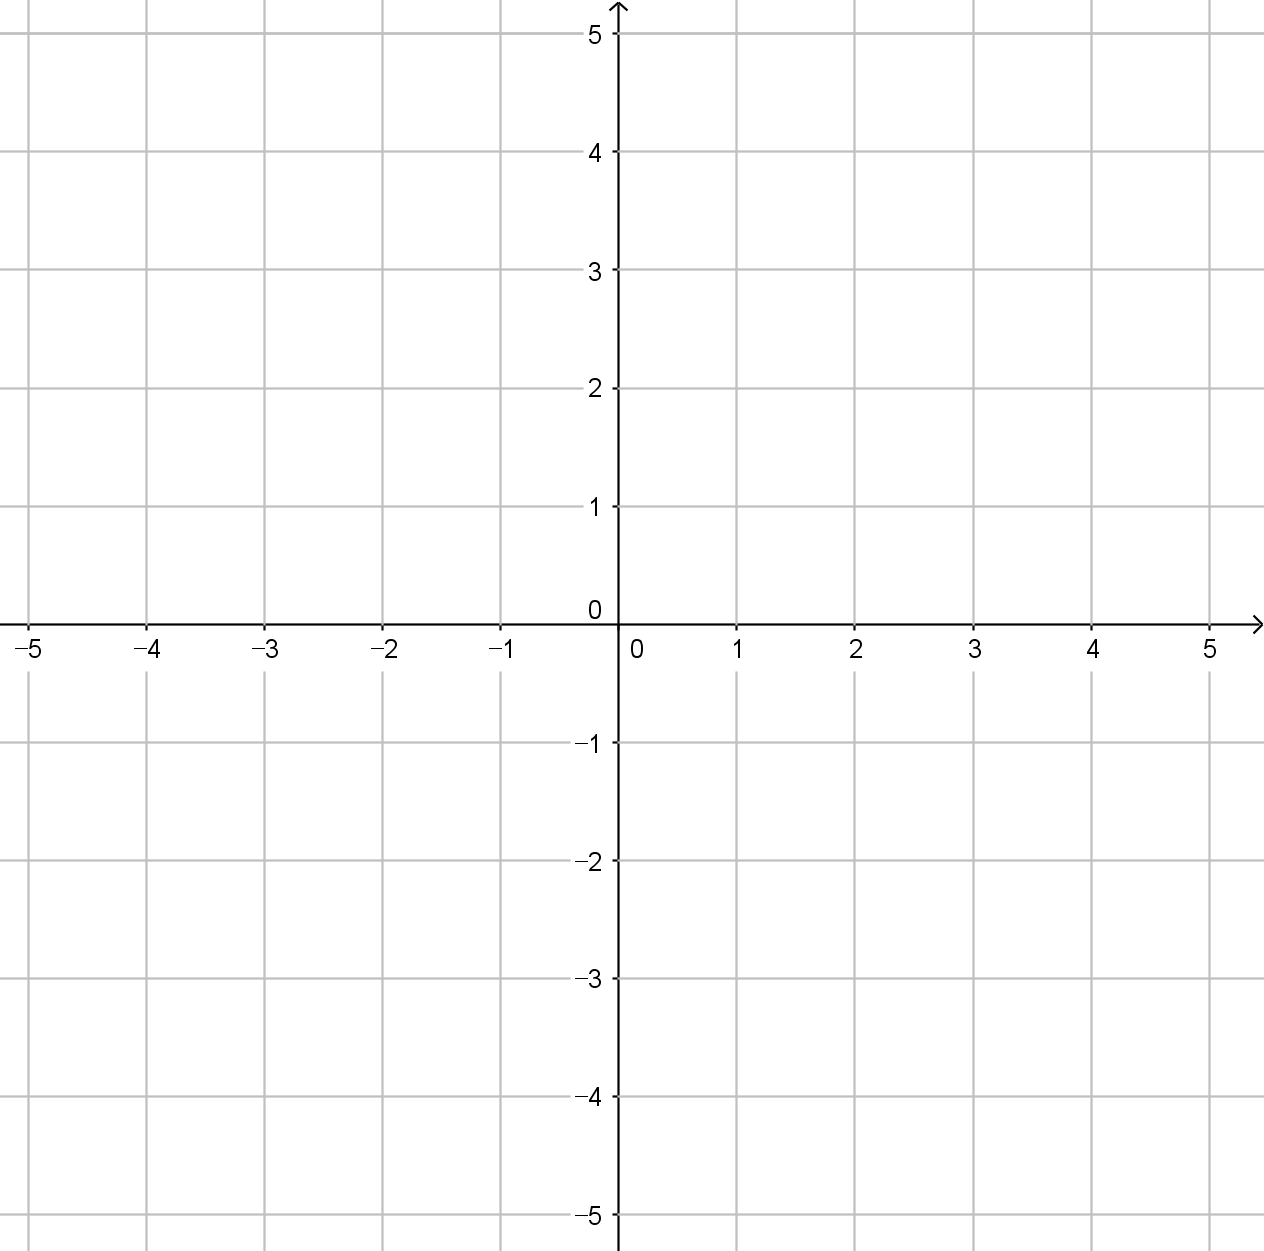
\includegraphics[width=0.9\textwidth]{55}
\end{minipage}
\begin{minipage}{0.45\textwidth}\centering
\(y=x^2+4x+3\)
\par\bigskip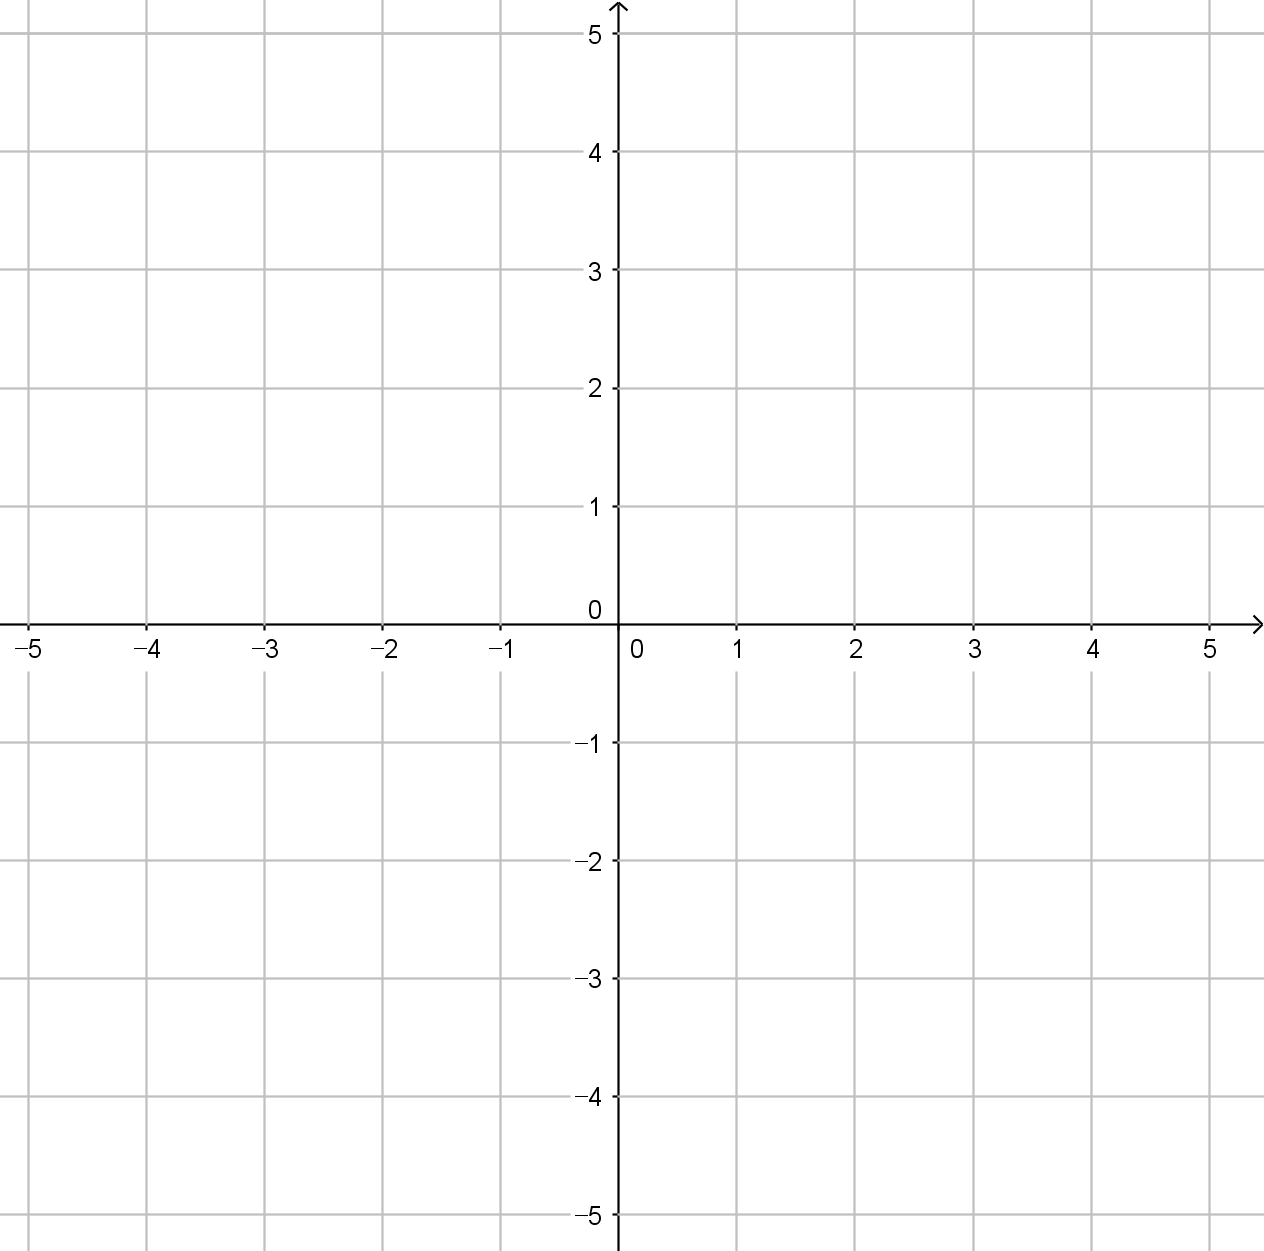
\includegraphics[width=0.9\textwidth]{55}
\end{minipage}\bigskip\bigskip\par
\begin{minipage}{0.45\textwidth}\centering
\(y=x^2+6x+5\)
\par\bigskip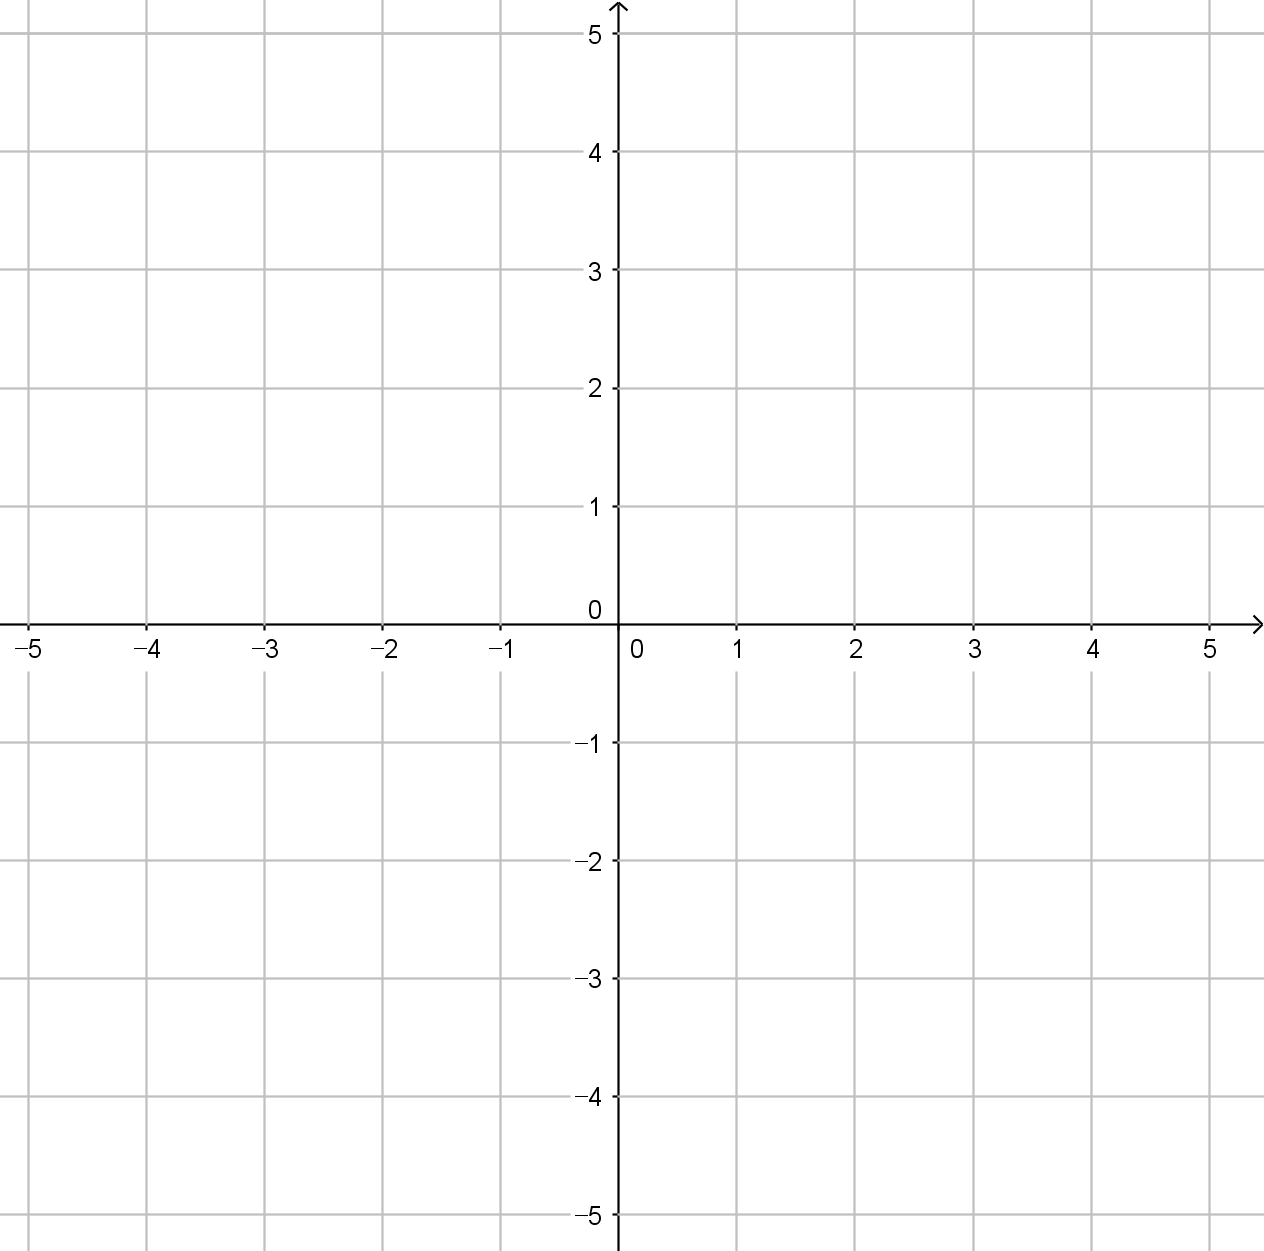
\includegraphics[width=0.9\textwidth]{55}
\end{minipage}
\begin{minipage}{0.45\textwidth}\centering
\(y=x^2-2x-3\)
\par\bigskip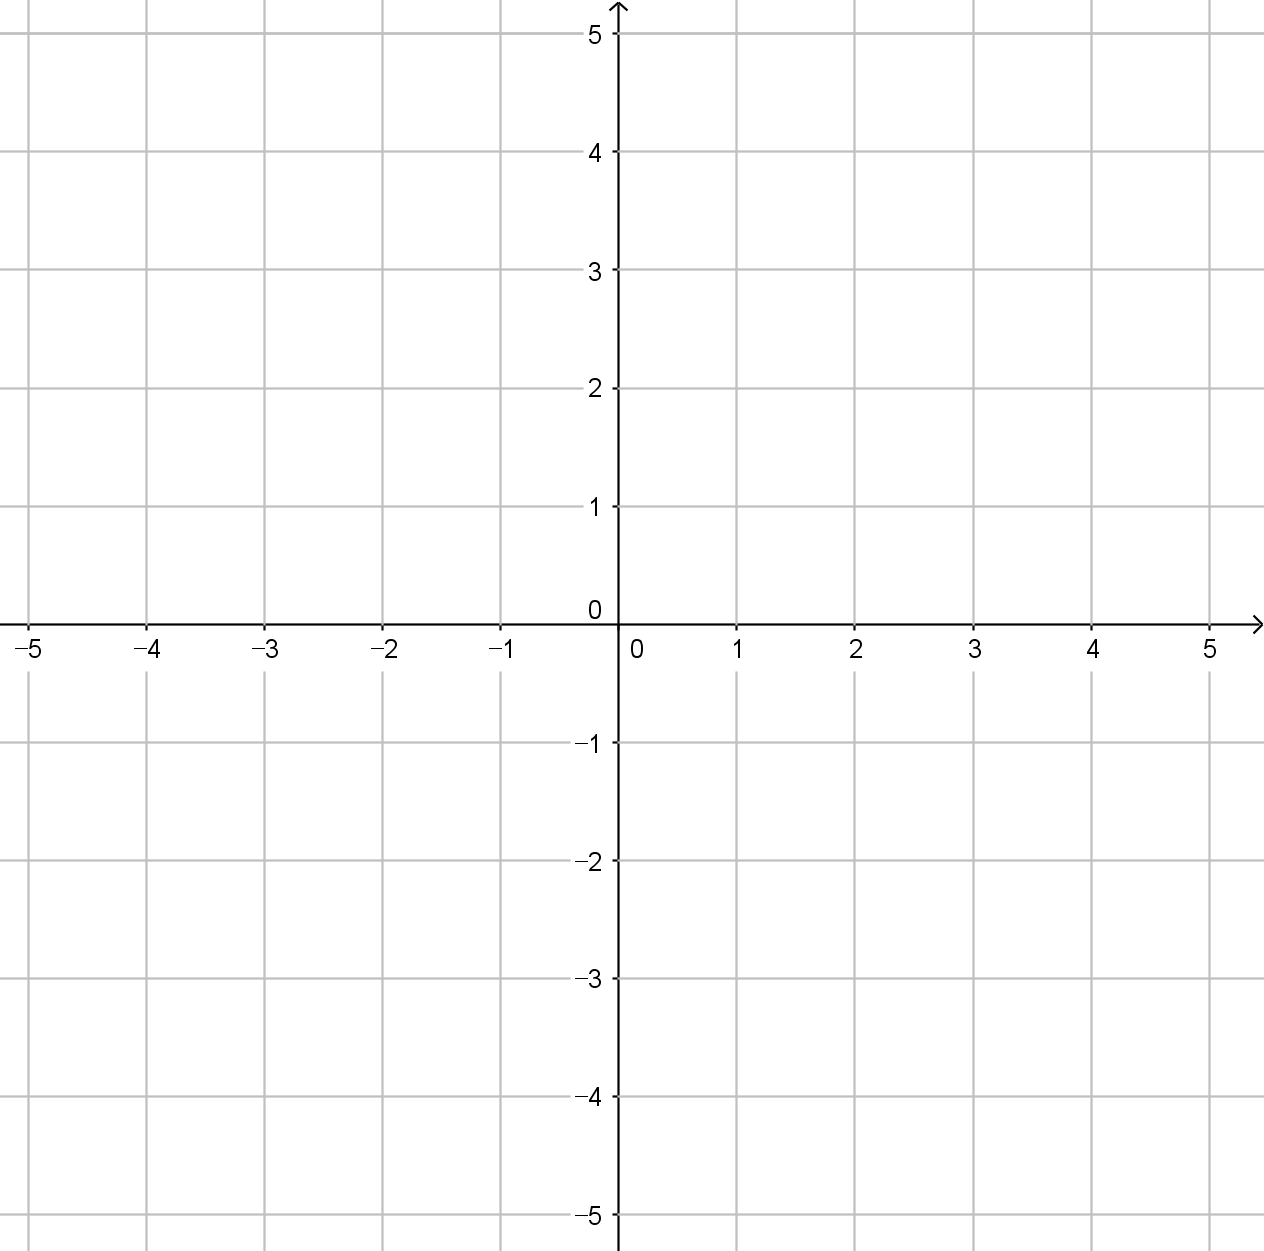
\includegraphics[width=0.9\textwidth]{55}
\end{minipage}\bigskip\bigskip\par

\clearpage
\begin{minipage}{0.45\textwidth}\centering
\(y=-x^2+2x-3\)
\par\bigskip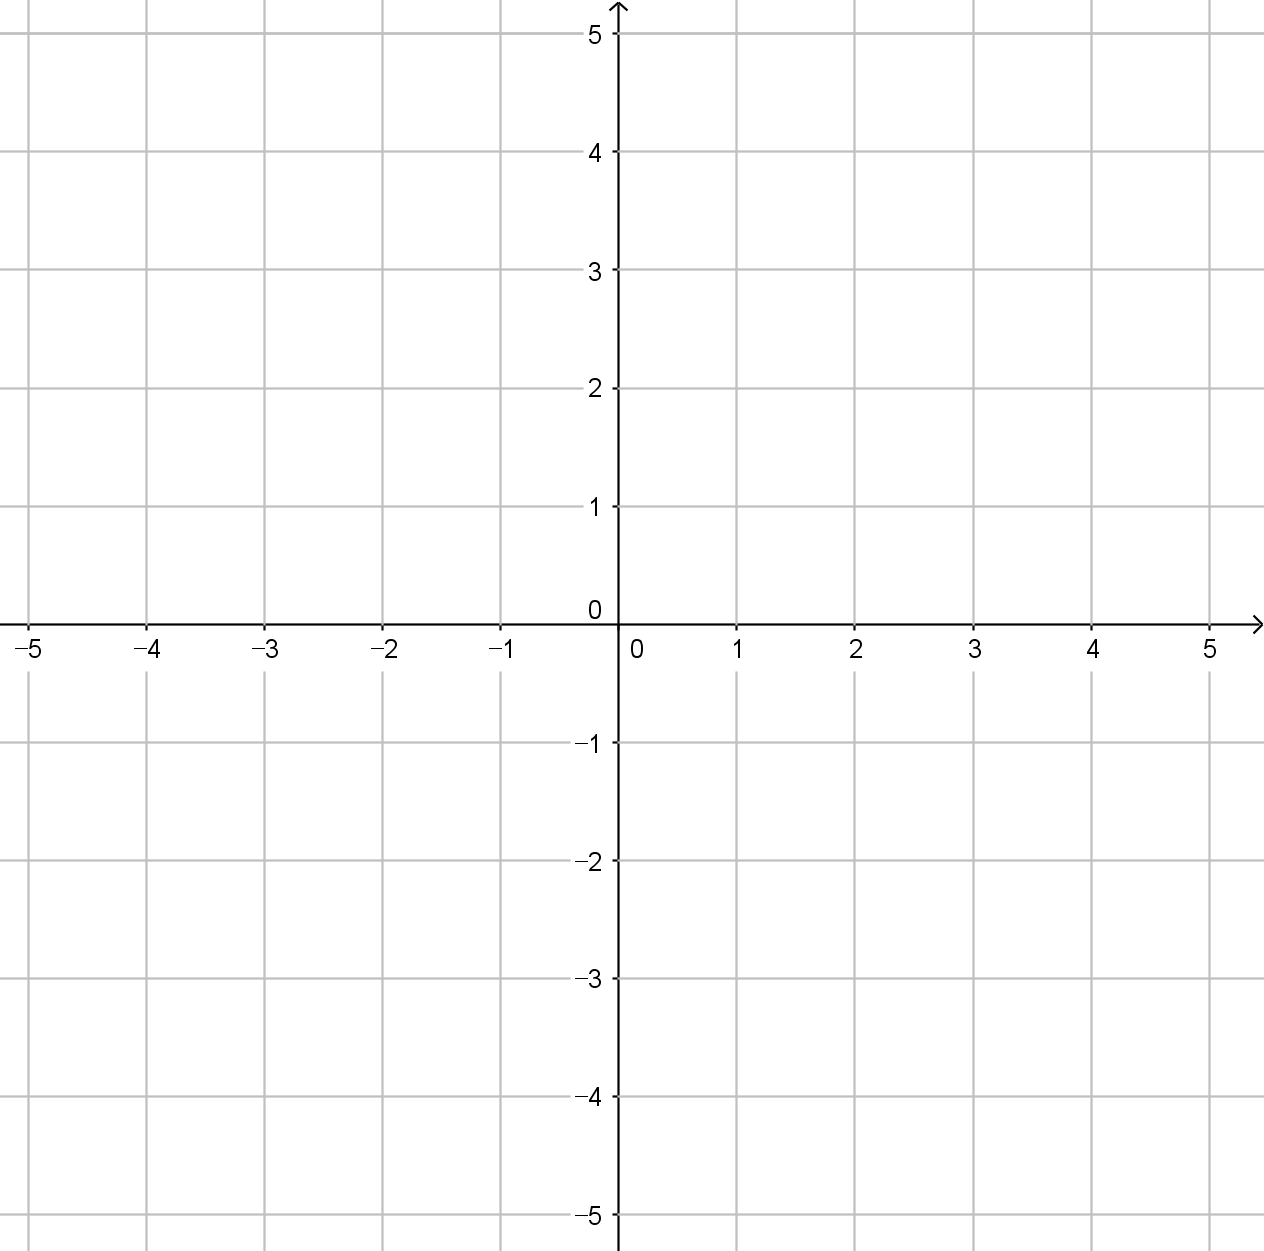
\includegraphics[width=0.9\textwidth]{55}
\end{minipage}
\begin{minipage}{0.45\textwidth}\centering
\(y=-x^2+4x-5\)
\par\bigskip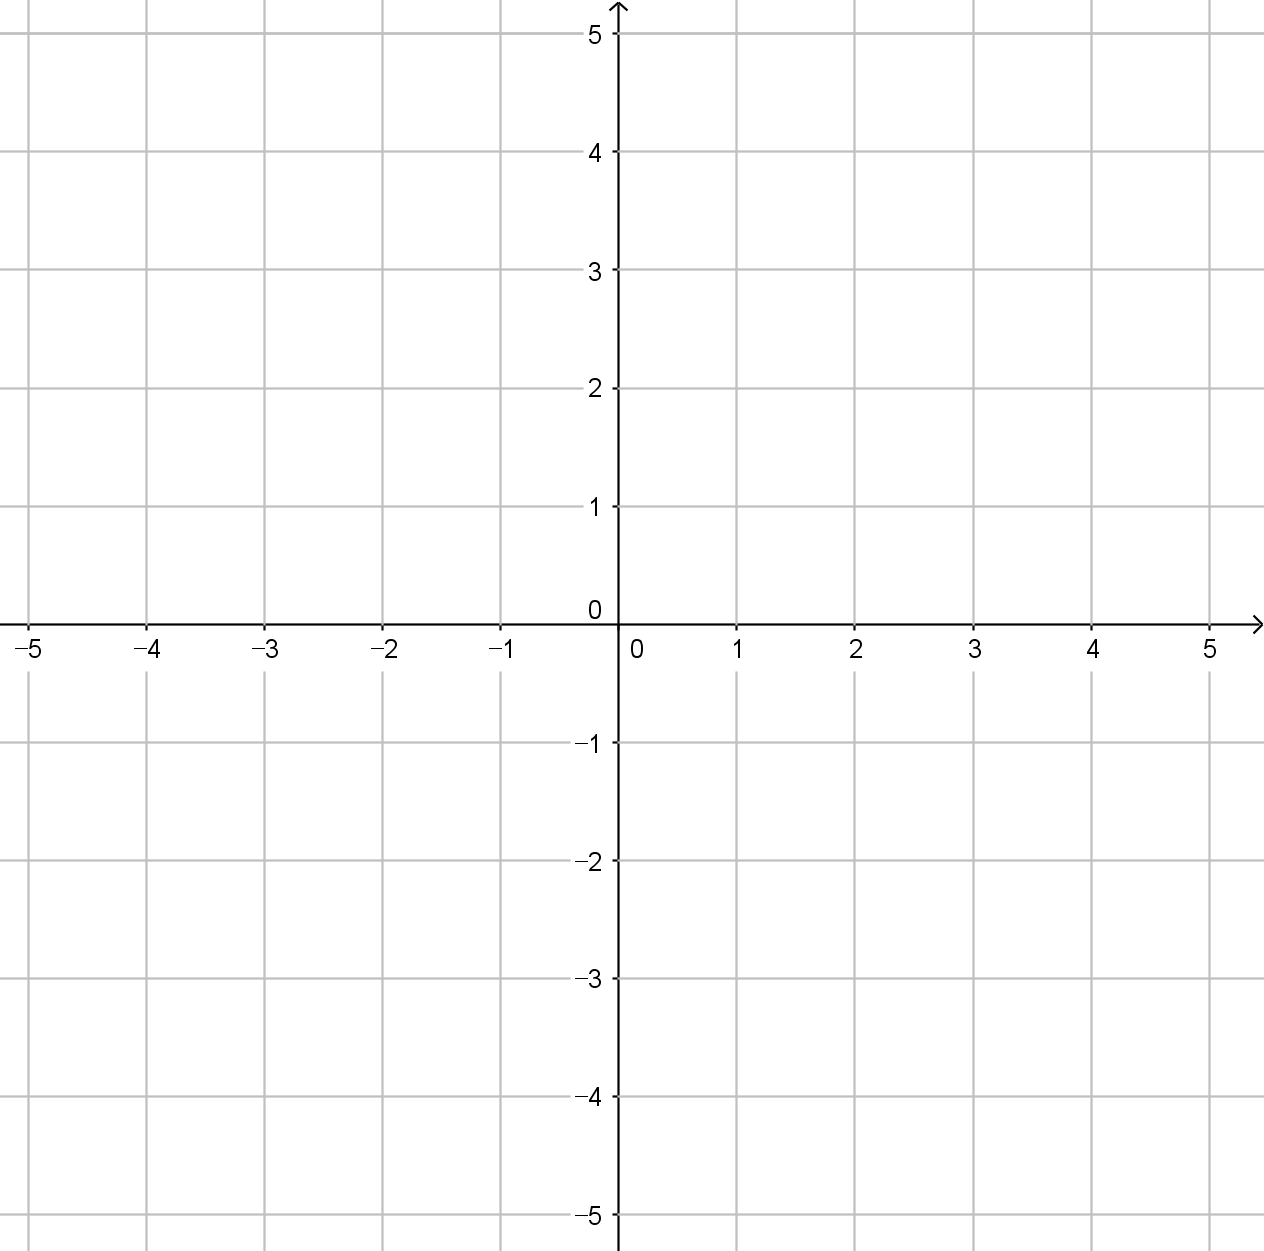
\includegraphics[width=0.9\textwidth]{55}
\end{minipage}\bigskip\bigskip\par
\begin{minipage}{0.45\textwidth}\centering
\(y=x^2-4x\)
\par\bigskip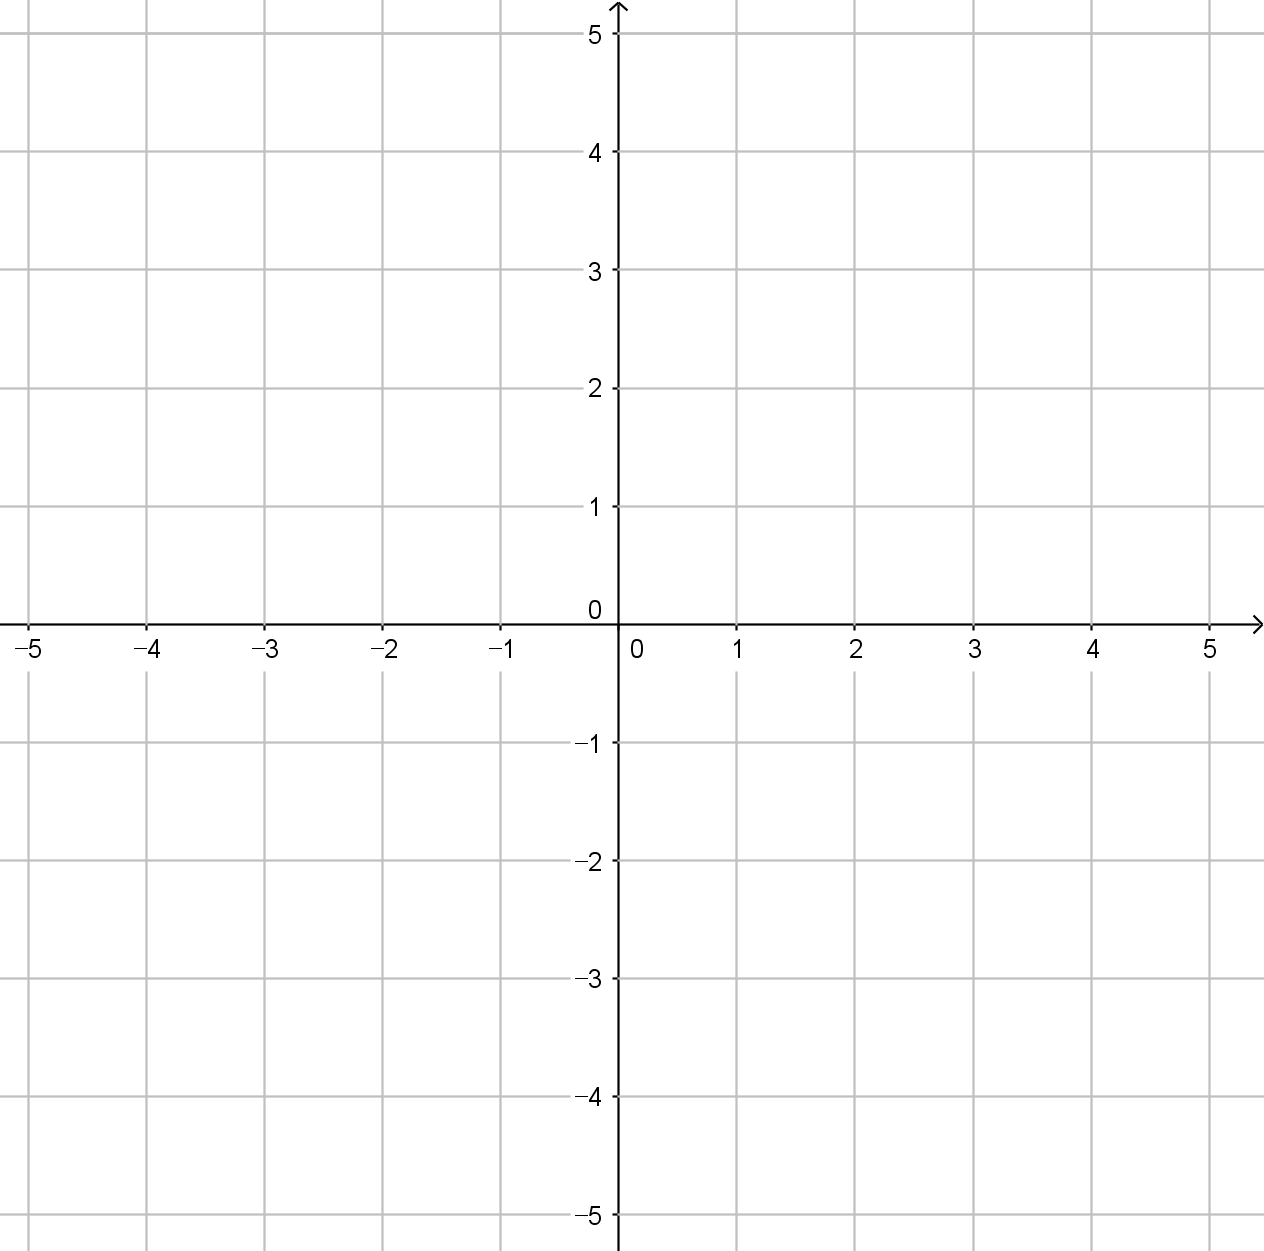
\includegraphics[width=0.9\textwidth]{55}
\end{minipage}
\begin{minipage}{0.45\textwidth}\centering
\(y=-x^2+2x\)
\par\bigskip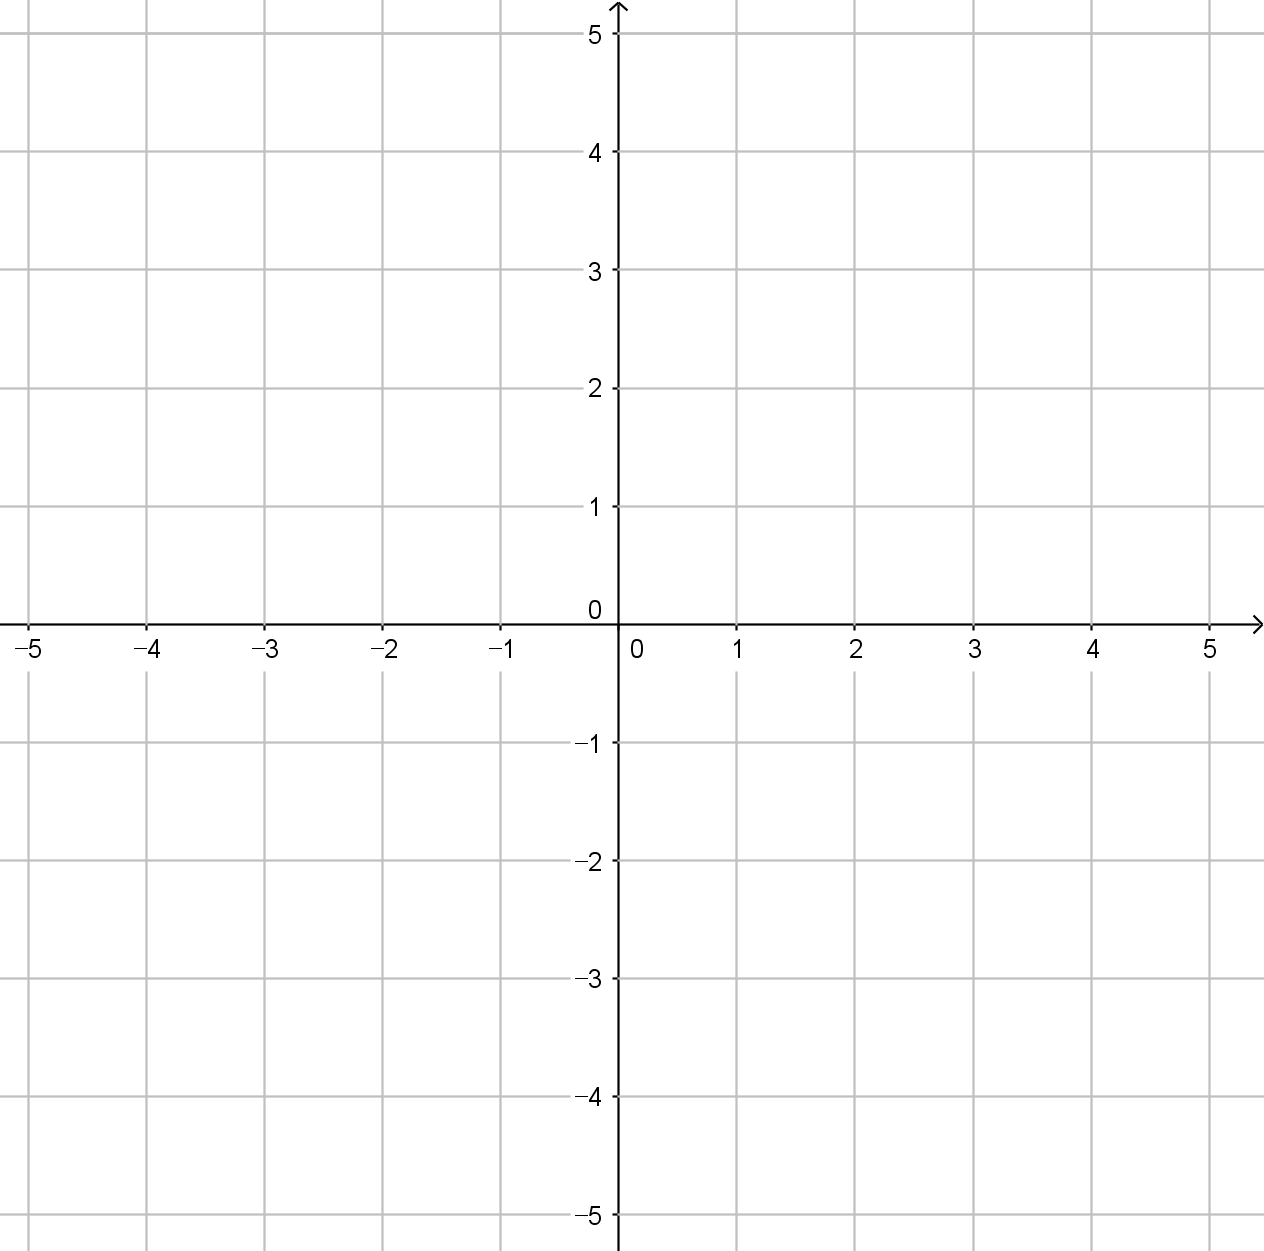
\includegraphics[width=0.9\textwidth]{55}
\end{minipage}\bigskip\bigskip\par
\begin{minipage}{0.45\textwidth}\centering
\(y=2x^2-4x+4\)
\par\bigskip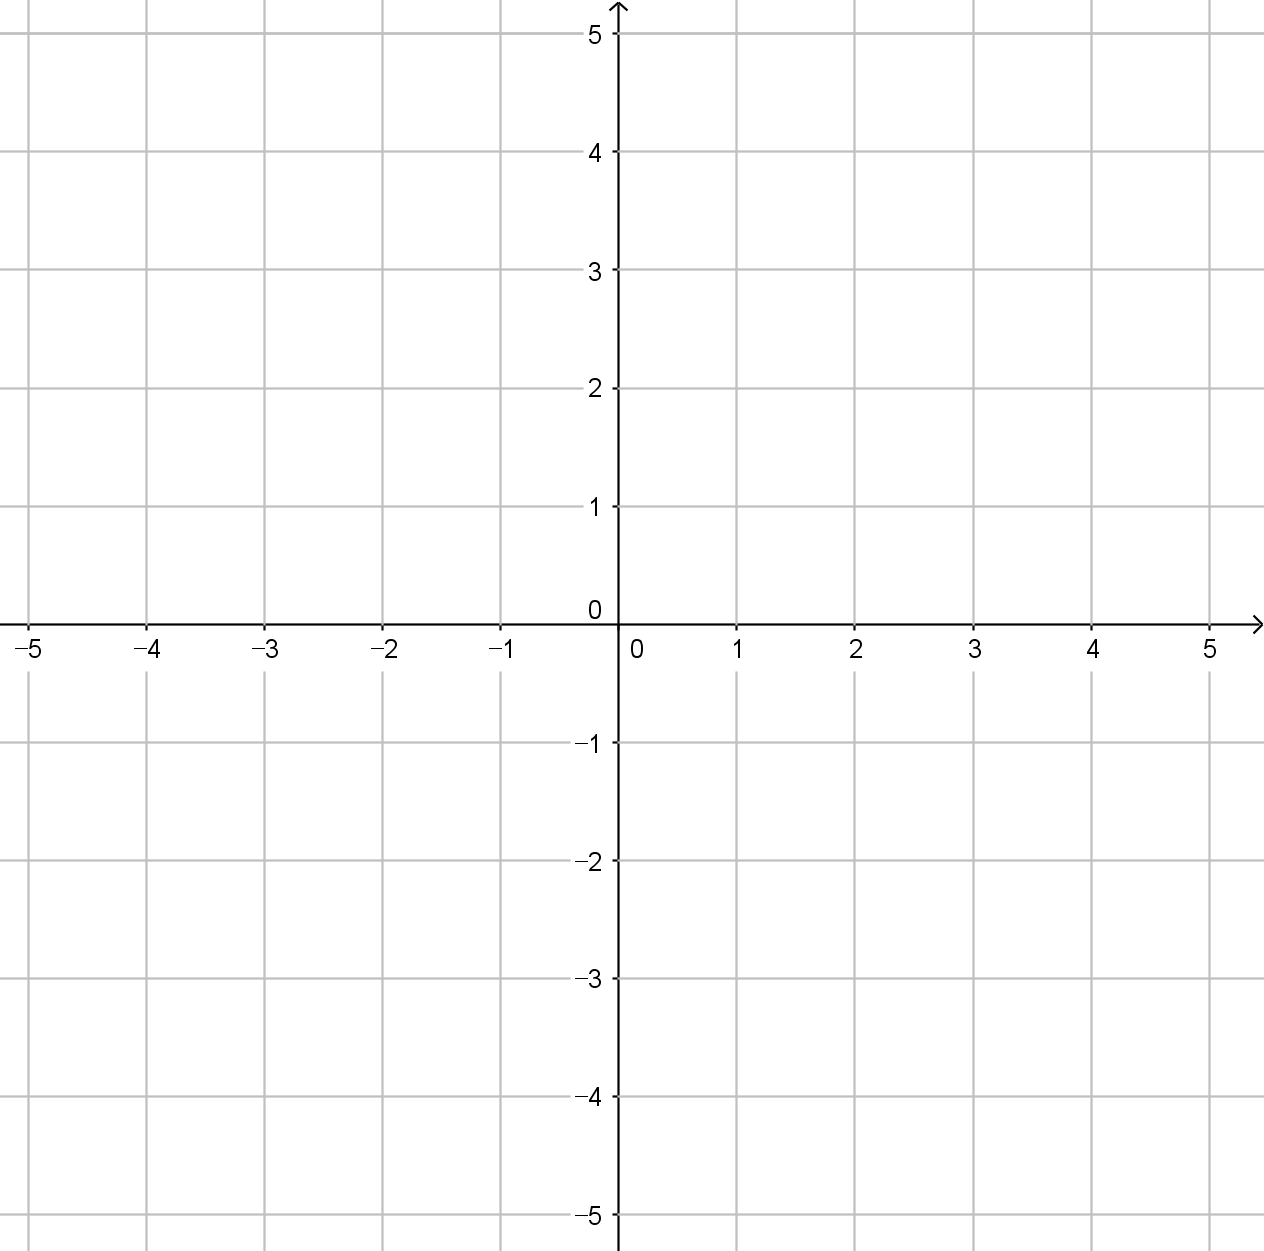
\includegraphics[width=0.9\textwidth]{55}
\end{minipage}
\begin{minipage}{0.45\textwidth}\centering
\(y=2x^2+8x+5\)
\par\bigskip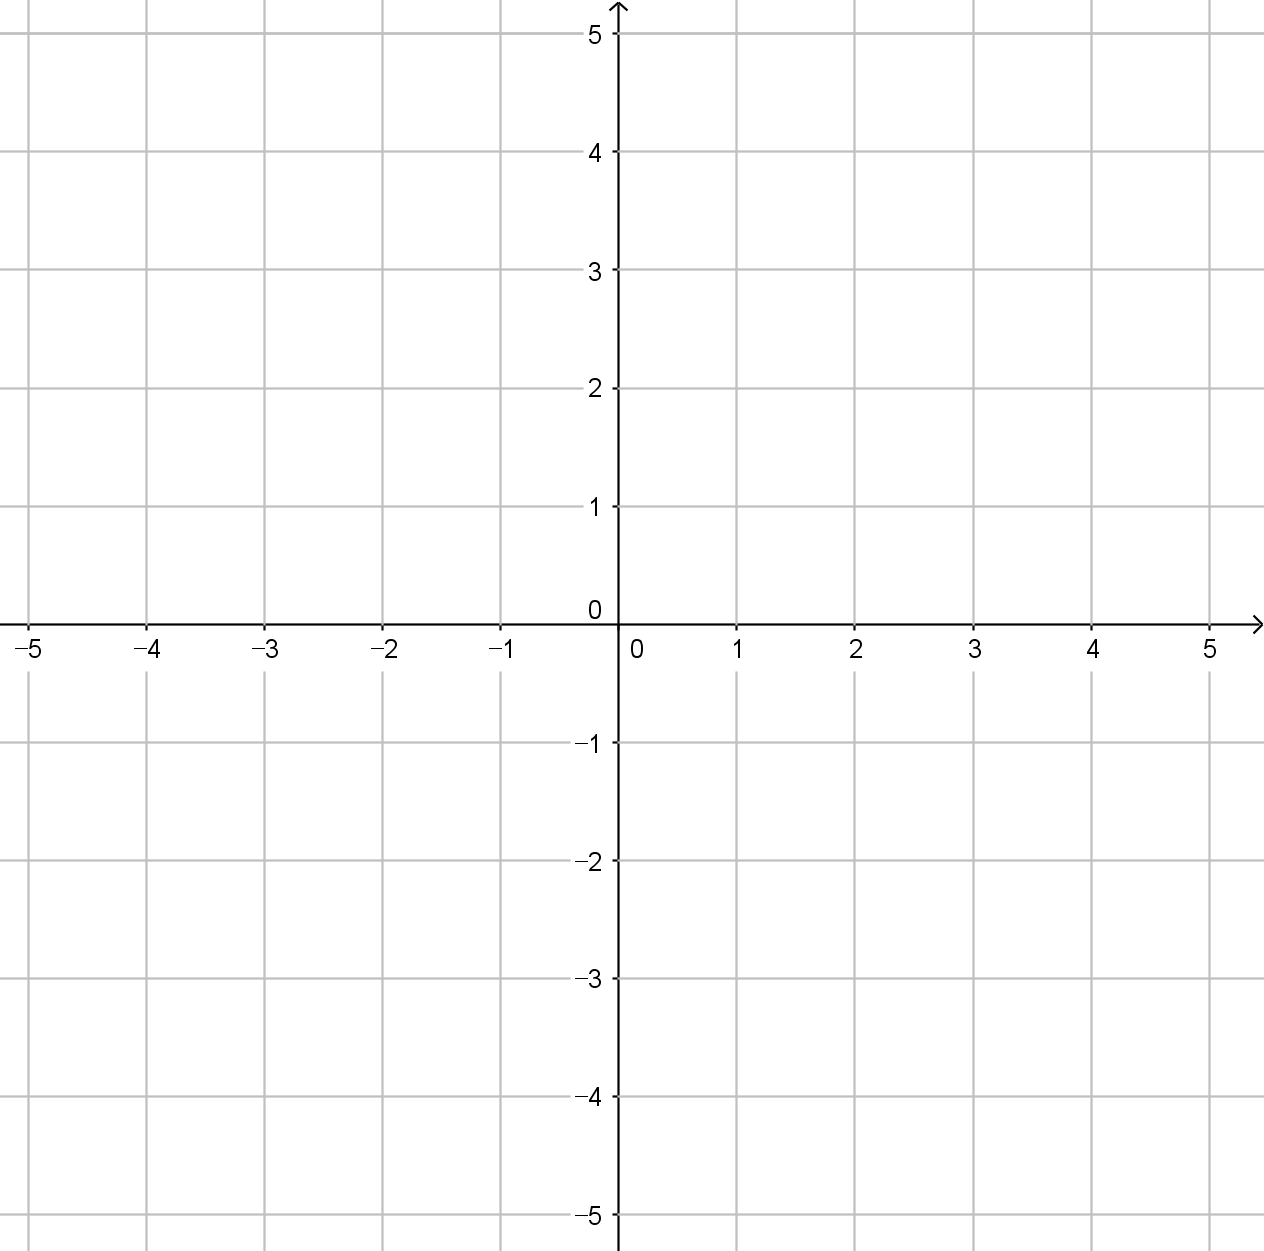
\includegraphics[width=0.9\textwidth]{55}
\end{minipage}\bigskip\bigskip\par

\clearpage
\begin{minipage}{0.45\textwidth}\centering
\(y=-2x^2-4x\)
\par\bigskip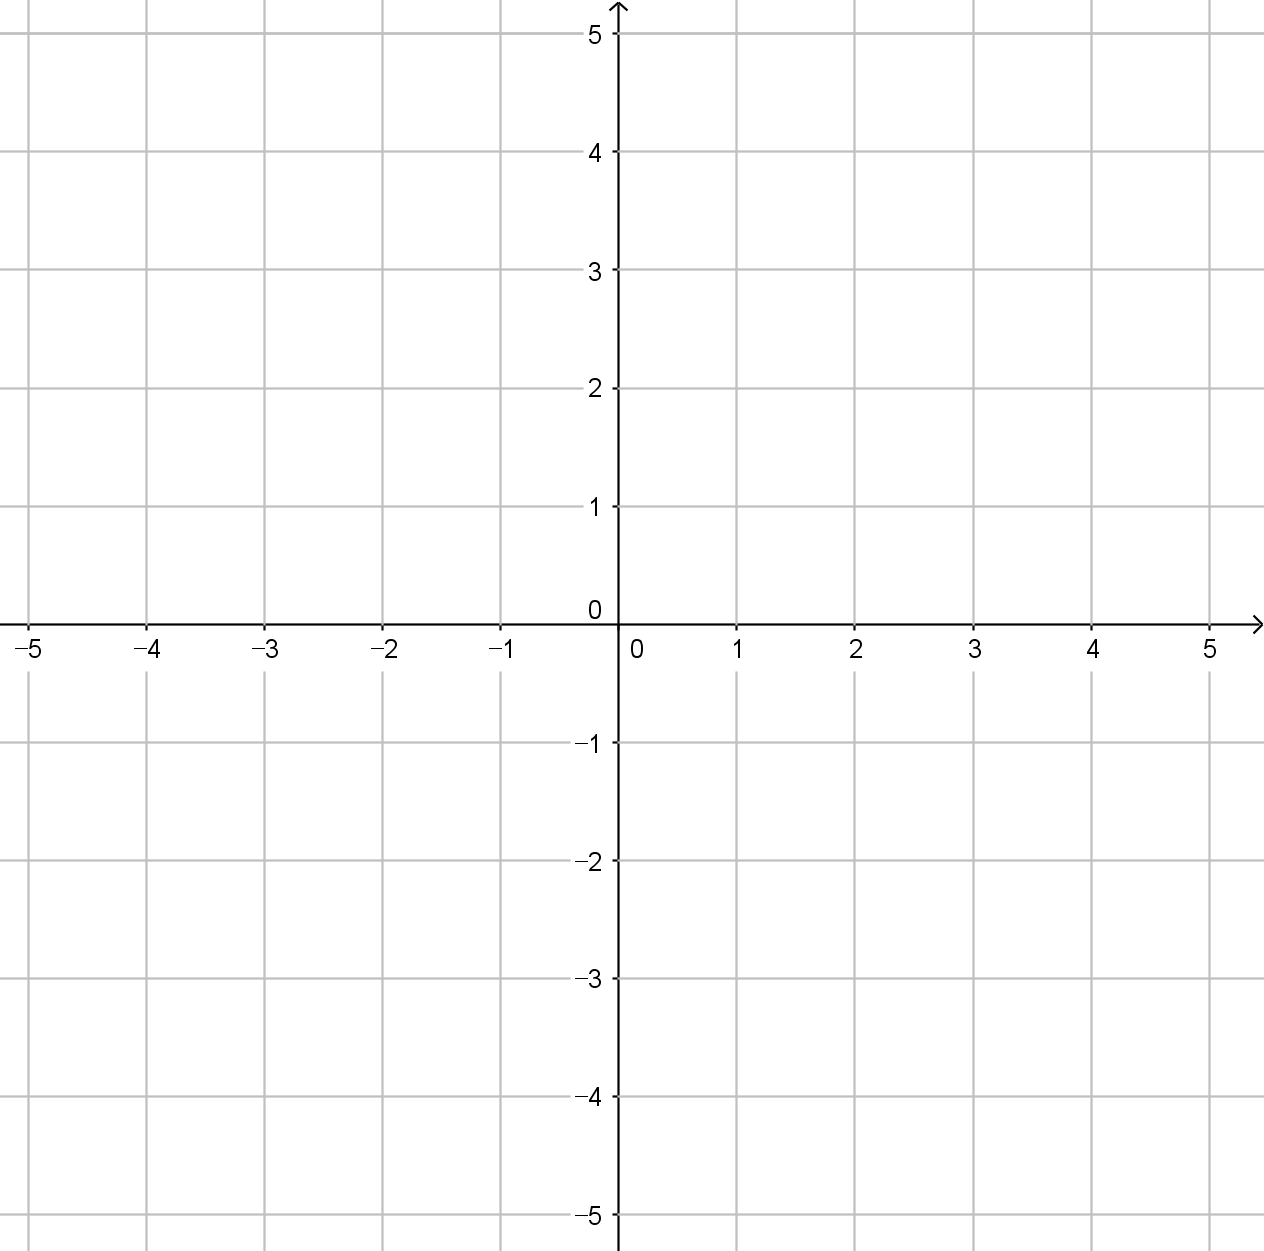
\includegraphics[width=0.9\textwidth]{55}
\end{minipage}
\begin{minipage}{0.45\textwidth}\centering
\(y=-2x^2+12x-16\)
\par\bigskip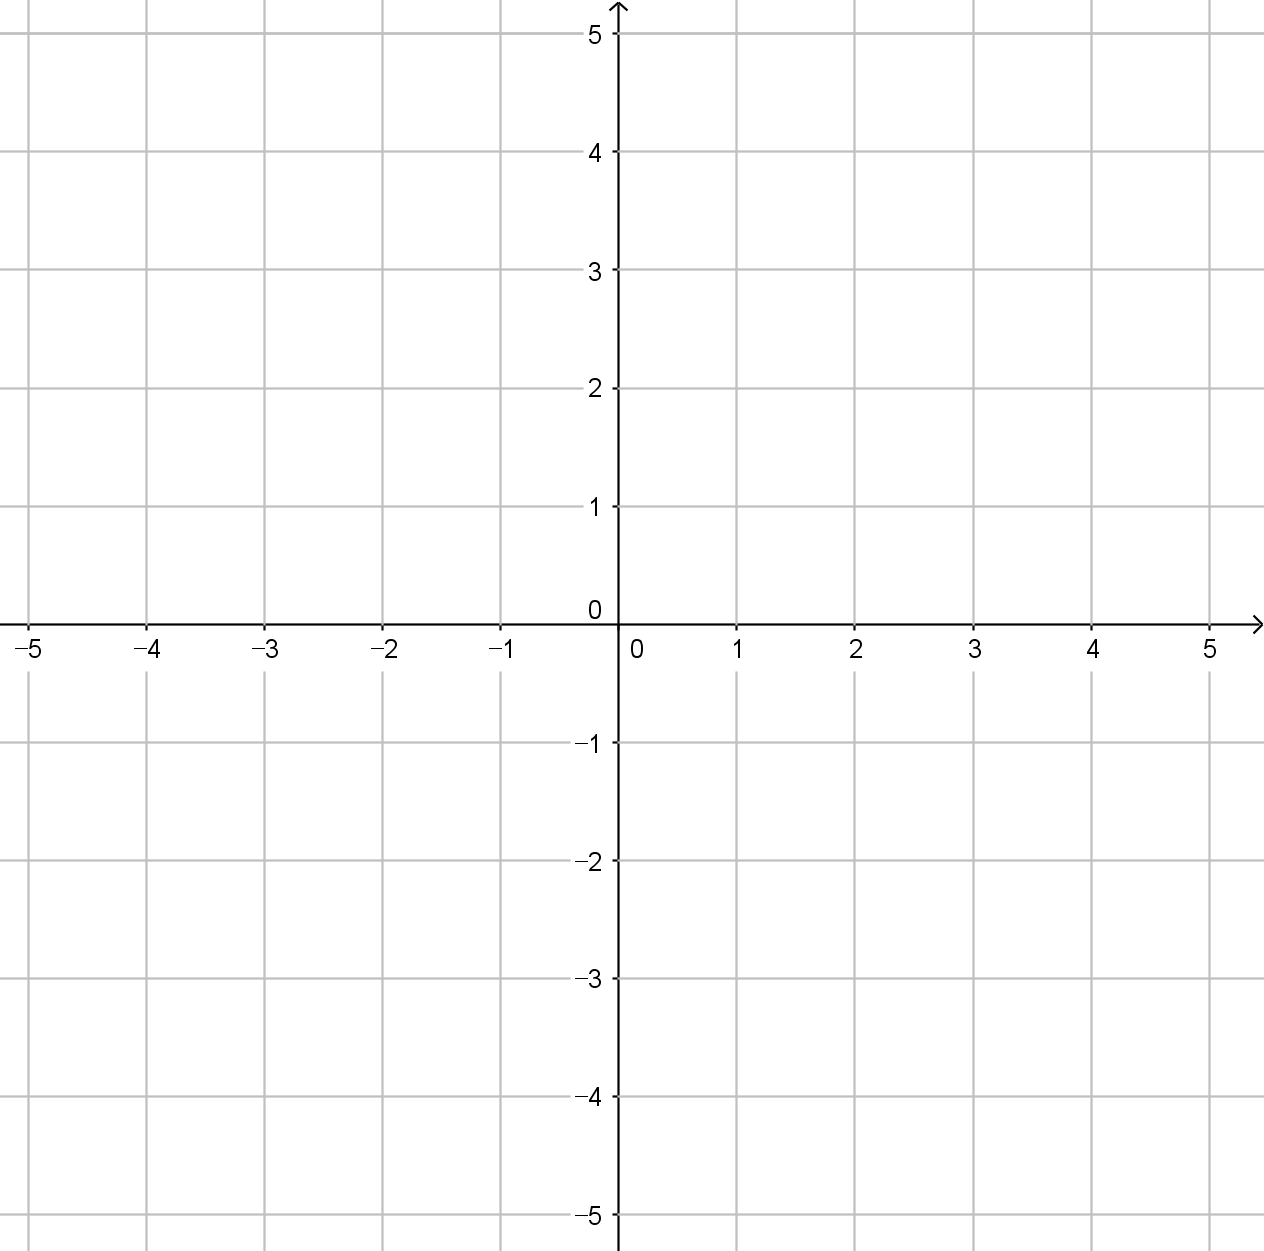
\includegraphics[width=0.9\textwidth]{55}
\end{minipage}\bigskip\bigskip\par
\begin{minipage}{0.45\textwidth}\centering
\(y=3x^2-6x-1\)
\par\bigskip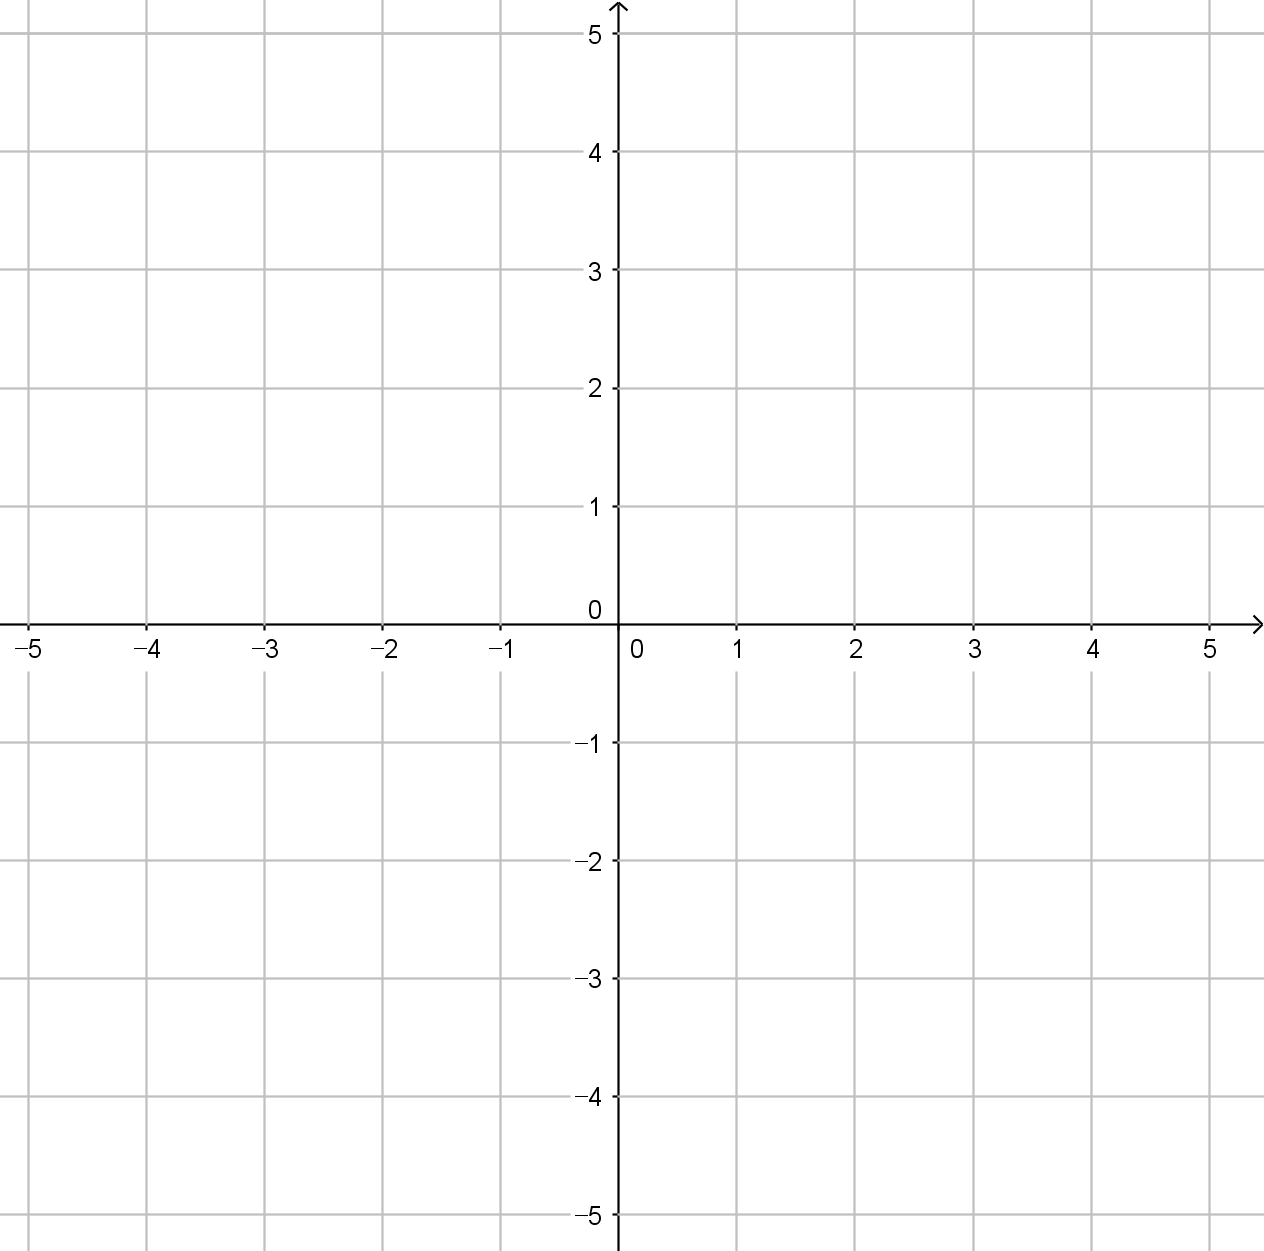
\includegraphics[width=0.9\textwidth]{55}
\end{minipage}
\begin{minipage}{0.45\textwidth}\centering
\(y=-3x^2-12x-10\)
\par\bigskip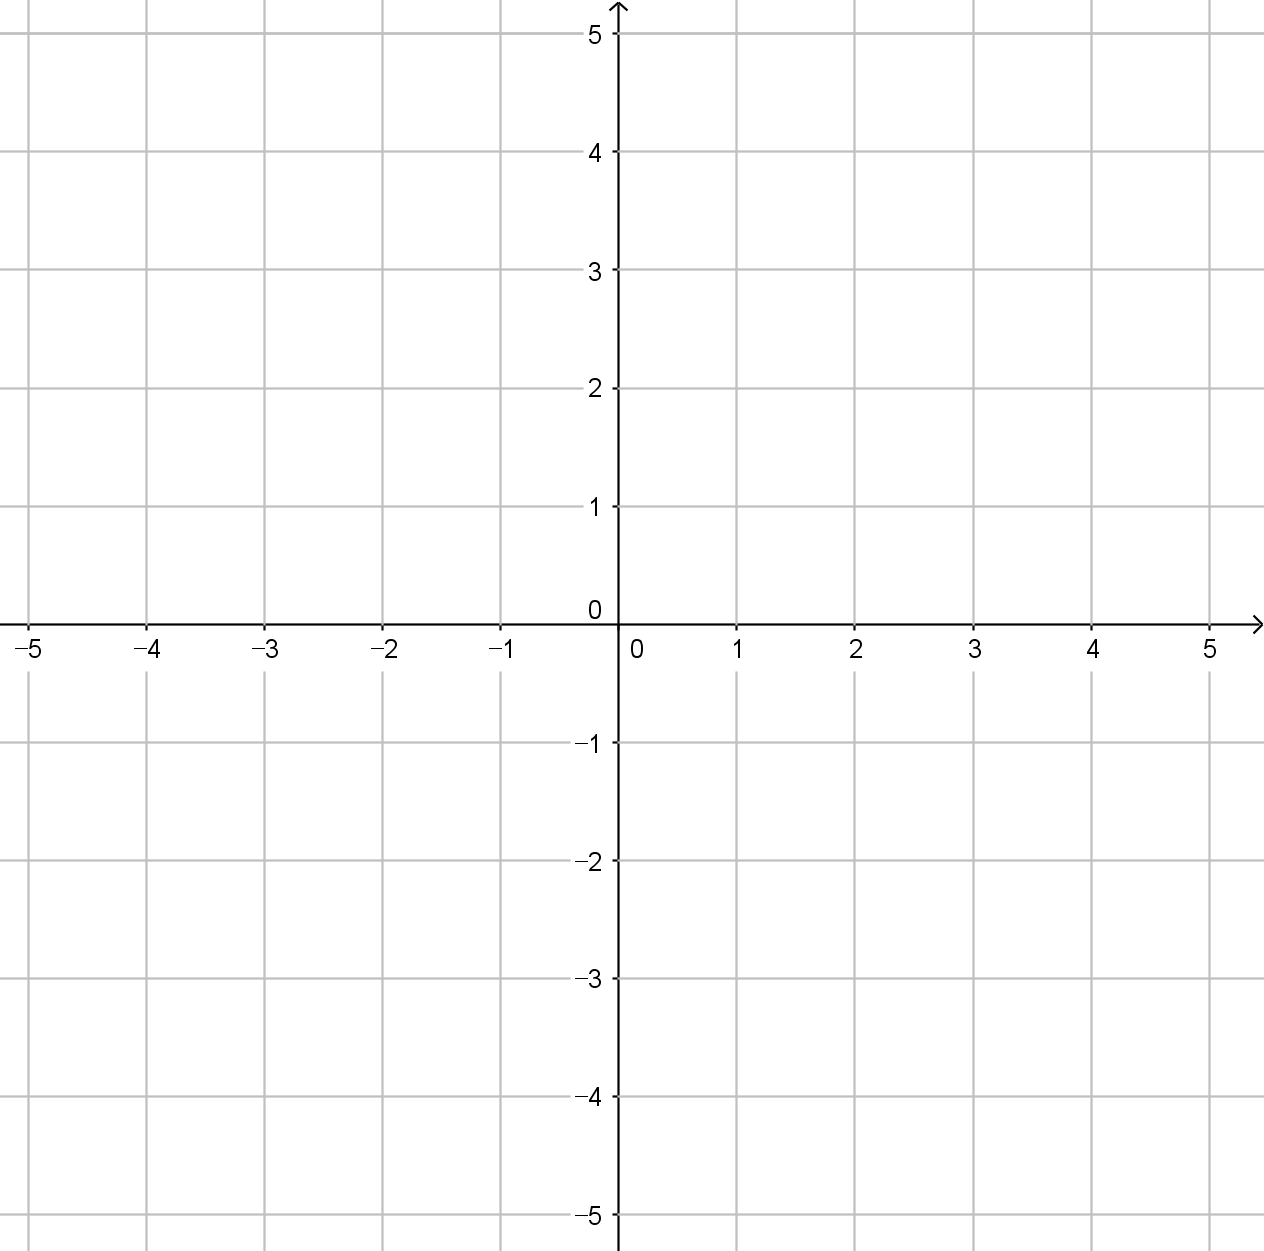
\includegraphics[width=0.9\textwidth]{55}
\end{minipage}\bigskip\bigskip\par
\begin{minipage}{0.45\textwidth}\centering
\(y=\frac12x^2-2x+3\)
\par\bigskip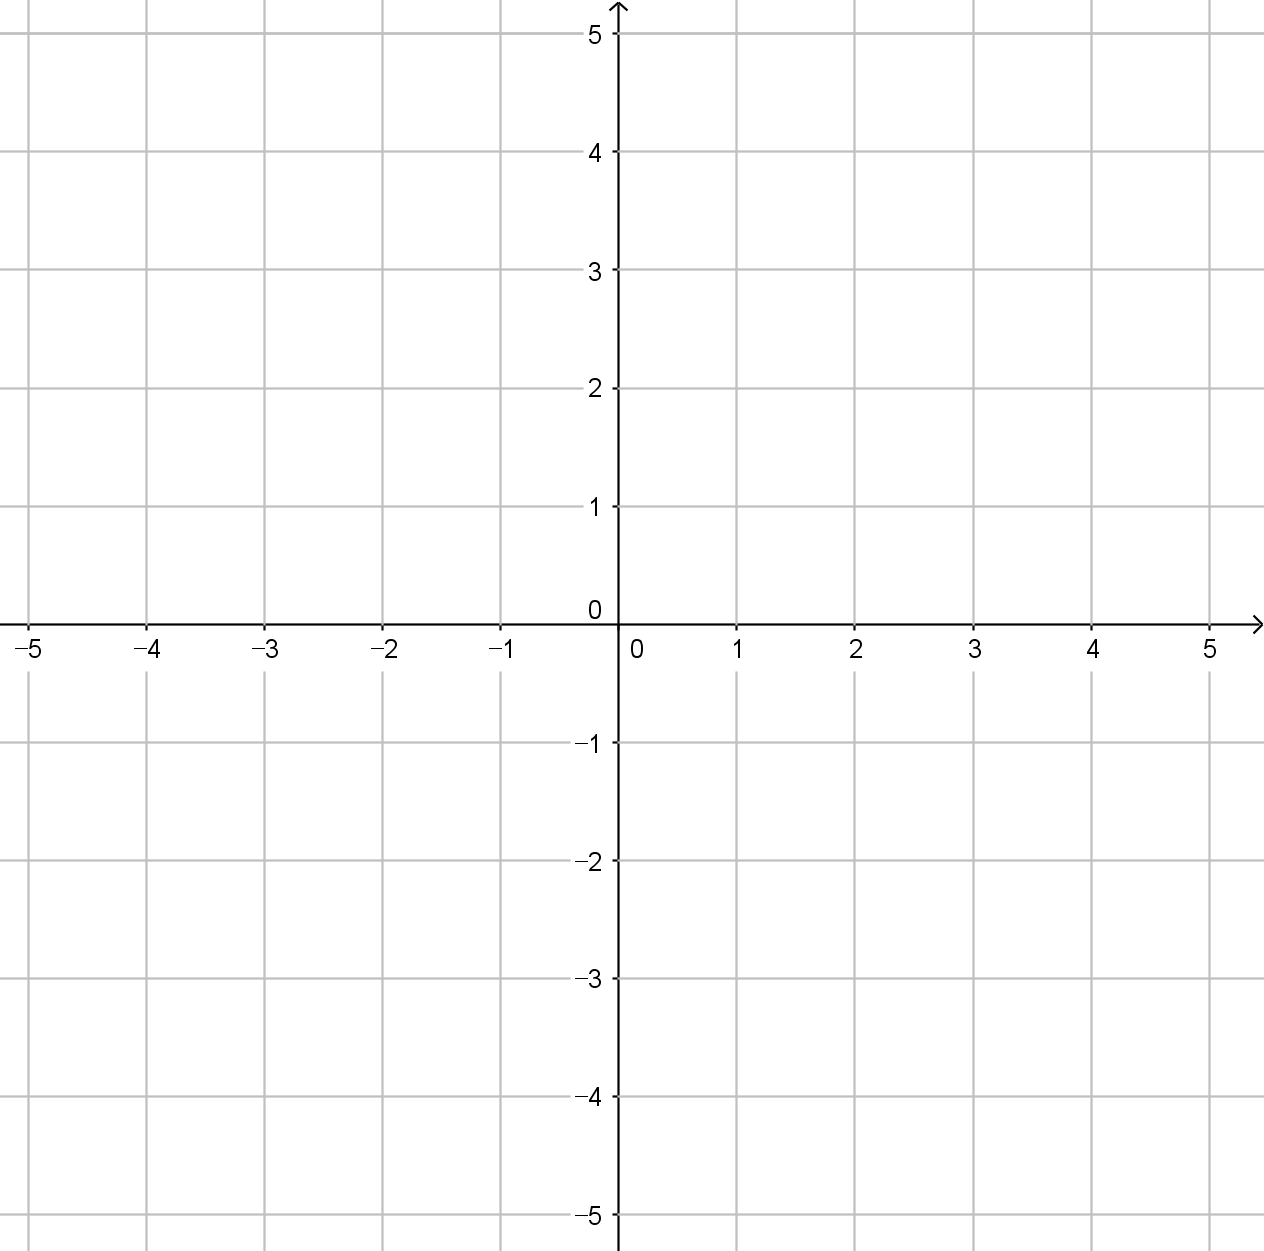
\includegraphics[width=0.9\textwidth]{55}
\end{minipage}
\begin{minipage}{0.45\textwidth}\centering
\(y=-\frac12x^2+4x-6\)
\par\bigskip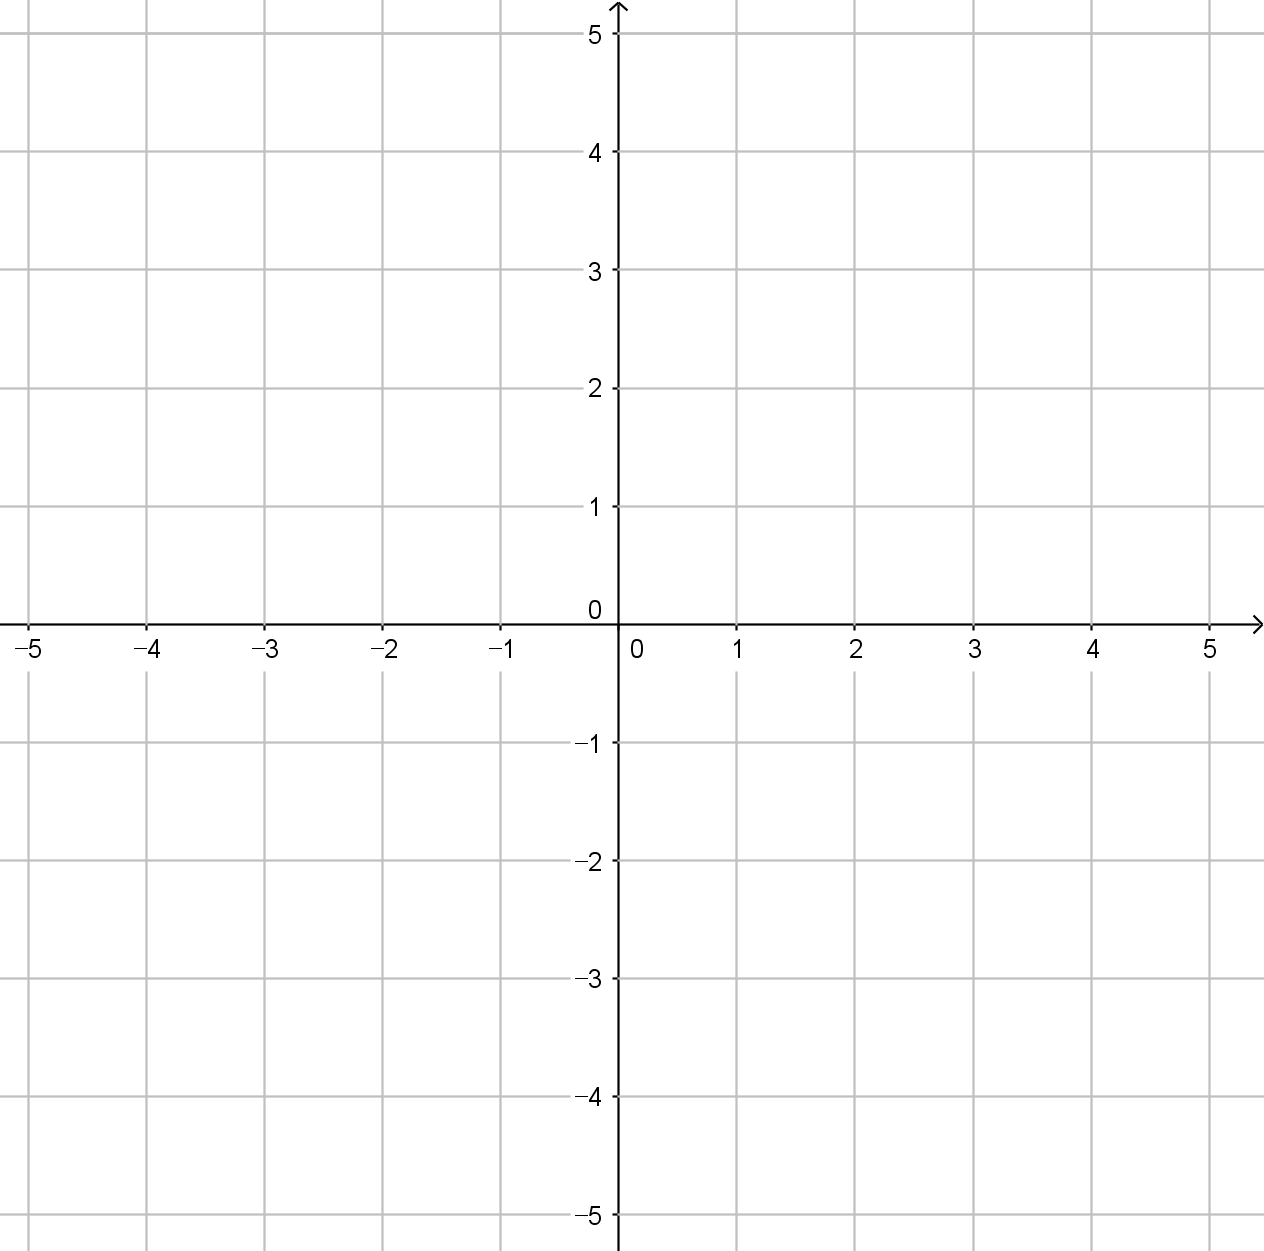
\includegraphics[width=0.9\textwidth]{55}
\end{minipage}\bigskip\bigskip\par

%%
\section*{답}

\begin{minipage}{0.45\textwidth}\centering
\(y=x^2\)
\par\bigskip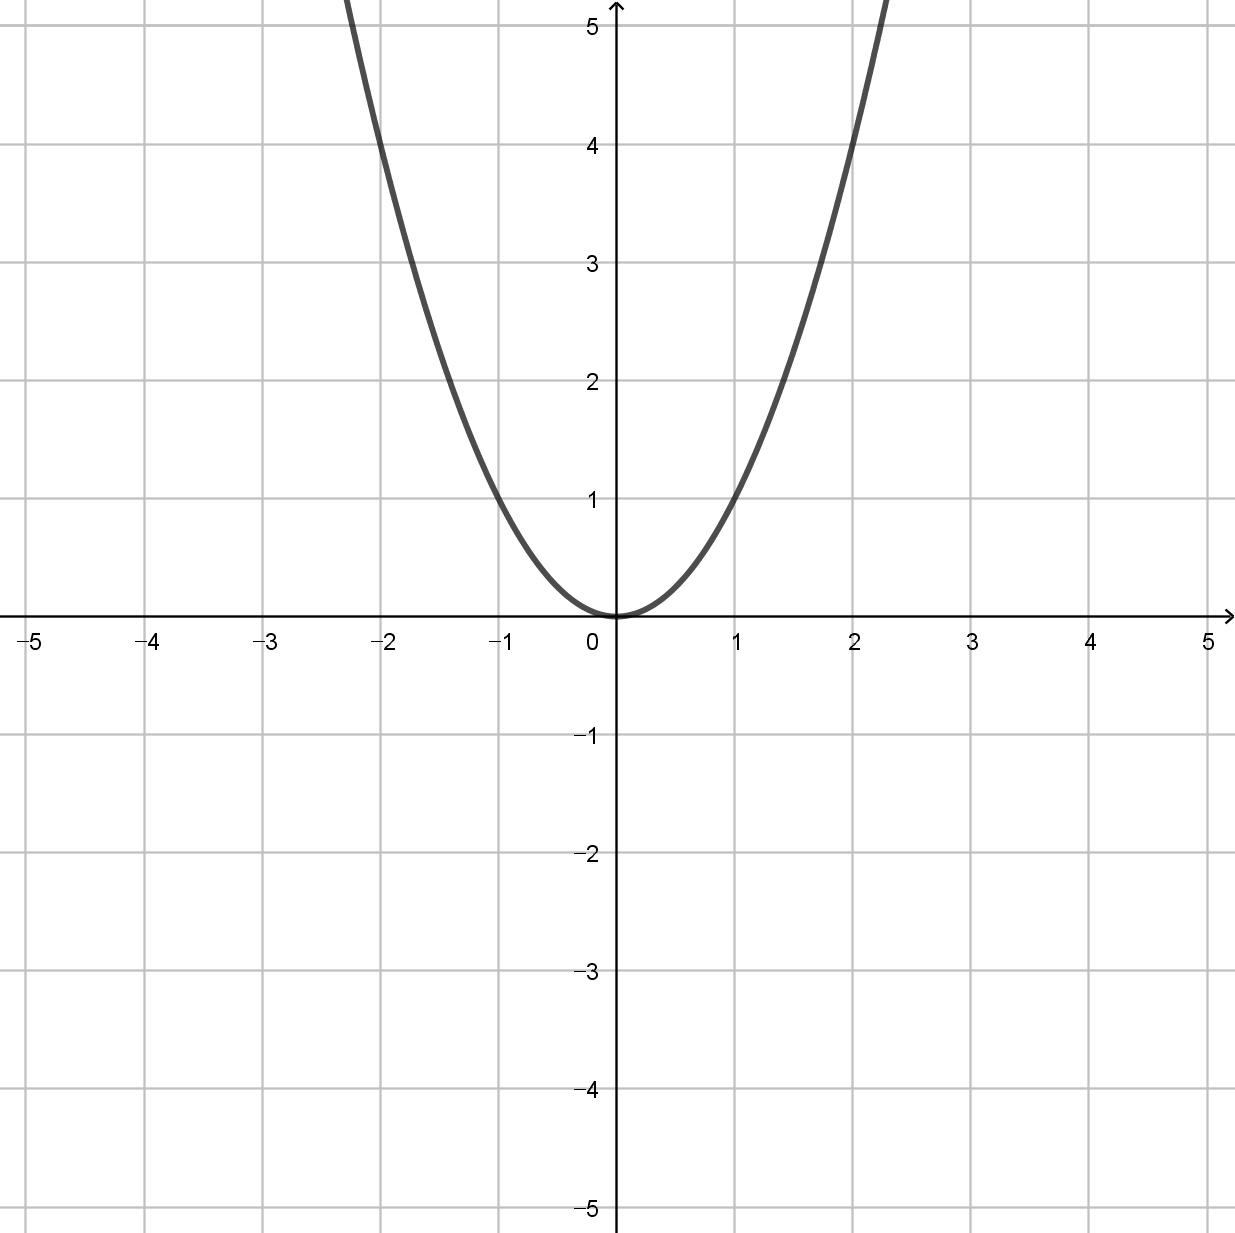
\includegraphics[width=0.9\textwidth]{img/2_quadratic_1}
\end{minipage}
\begin{minipage}{0.45\textwidth}\centering
\(y=-x^2\)
\par\bigskip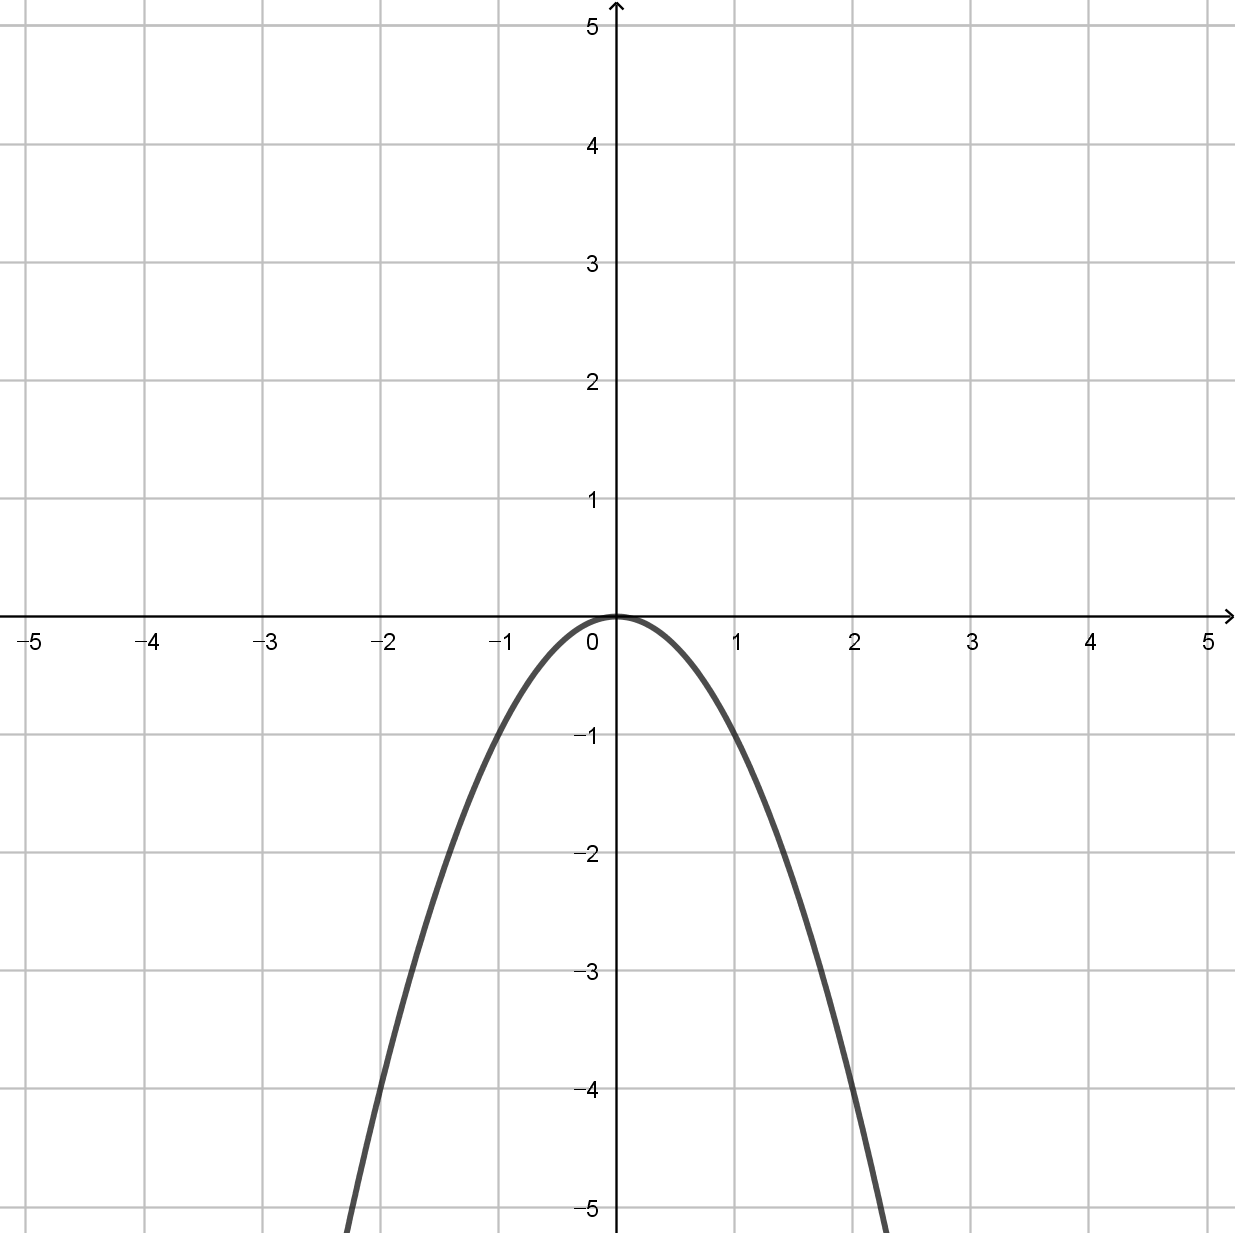
\includegraphics[width=0.9\textwidth]{img/2_quadratic_2}
\end{minipage}\bigskip\bigskip\par
\begin{minipage}{0.45\textwidth}\centering
\(y=2x^2\)
\par\bigskip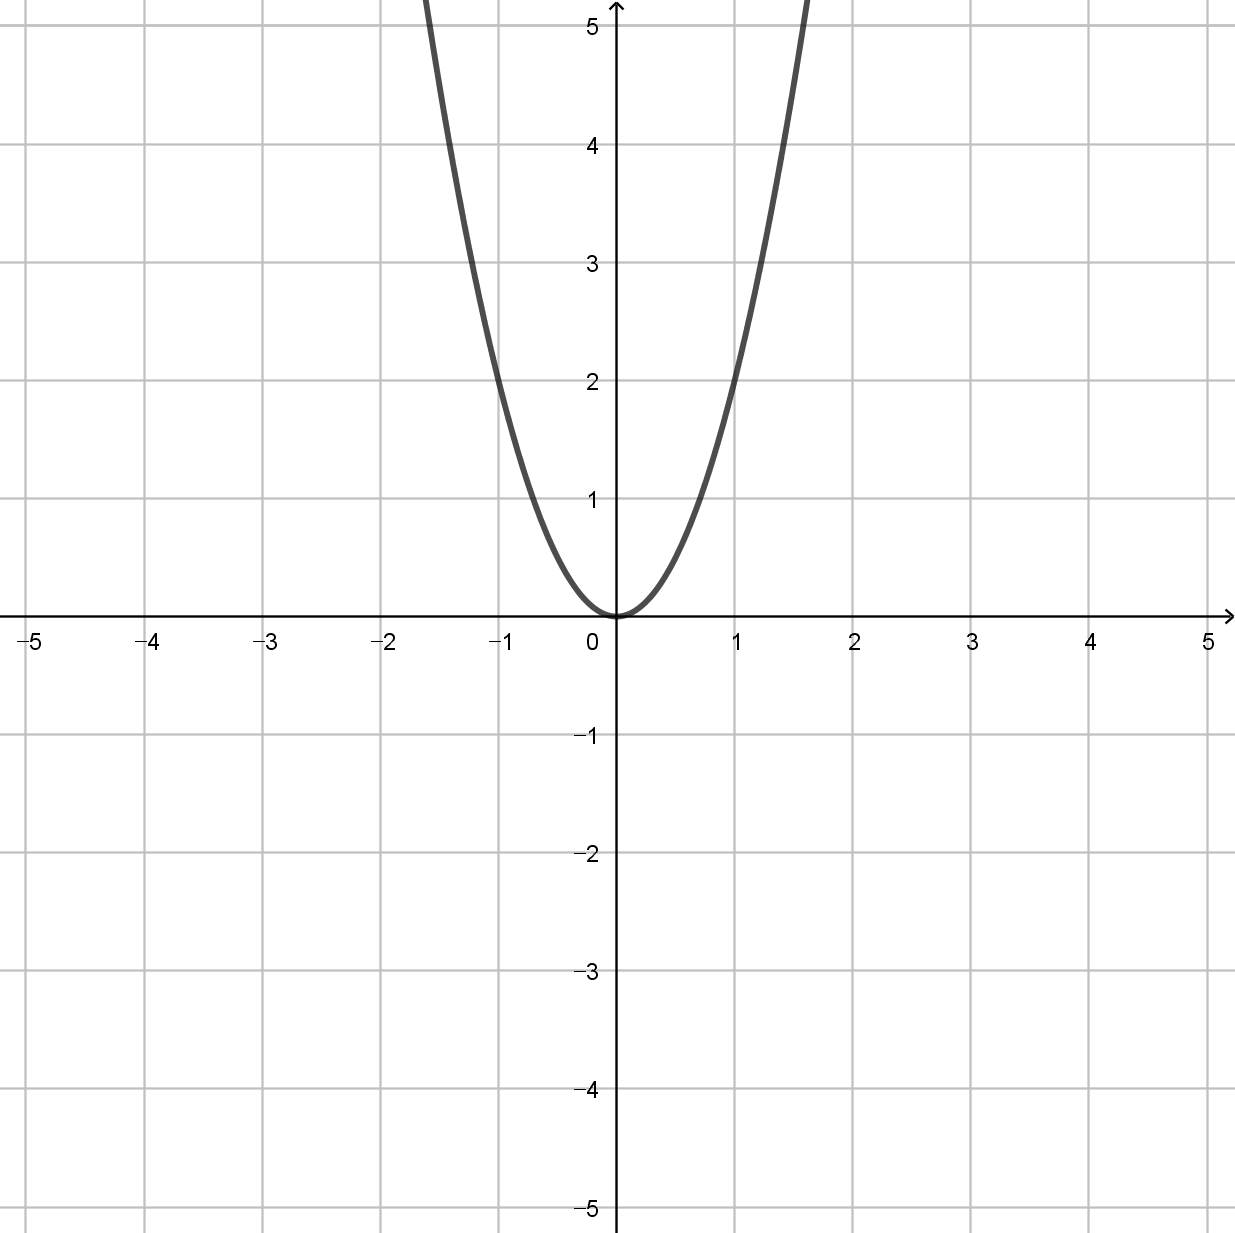
\includegraphics[width=0.9\textwidth]{img/2_quadratic_3}
\end{minipage}
\begin{minipage}{0.45\textwidth}\centering
\(y=-2x^2\)
\par\bigskip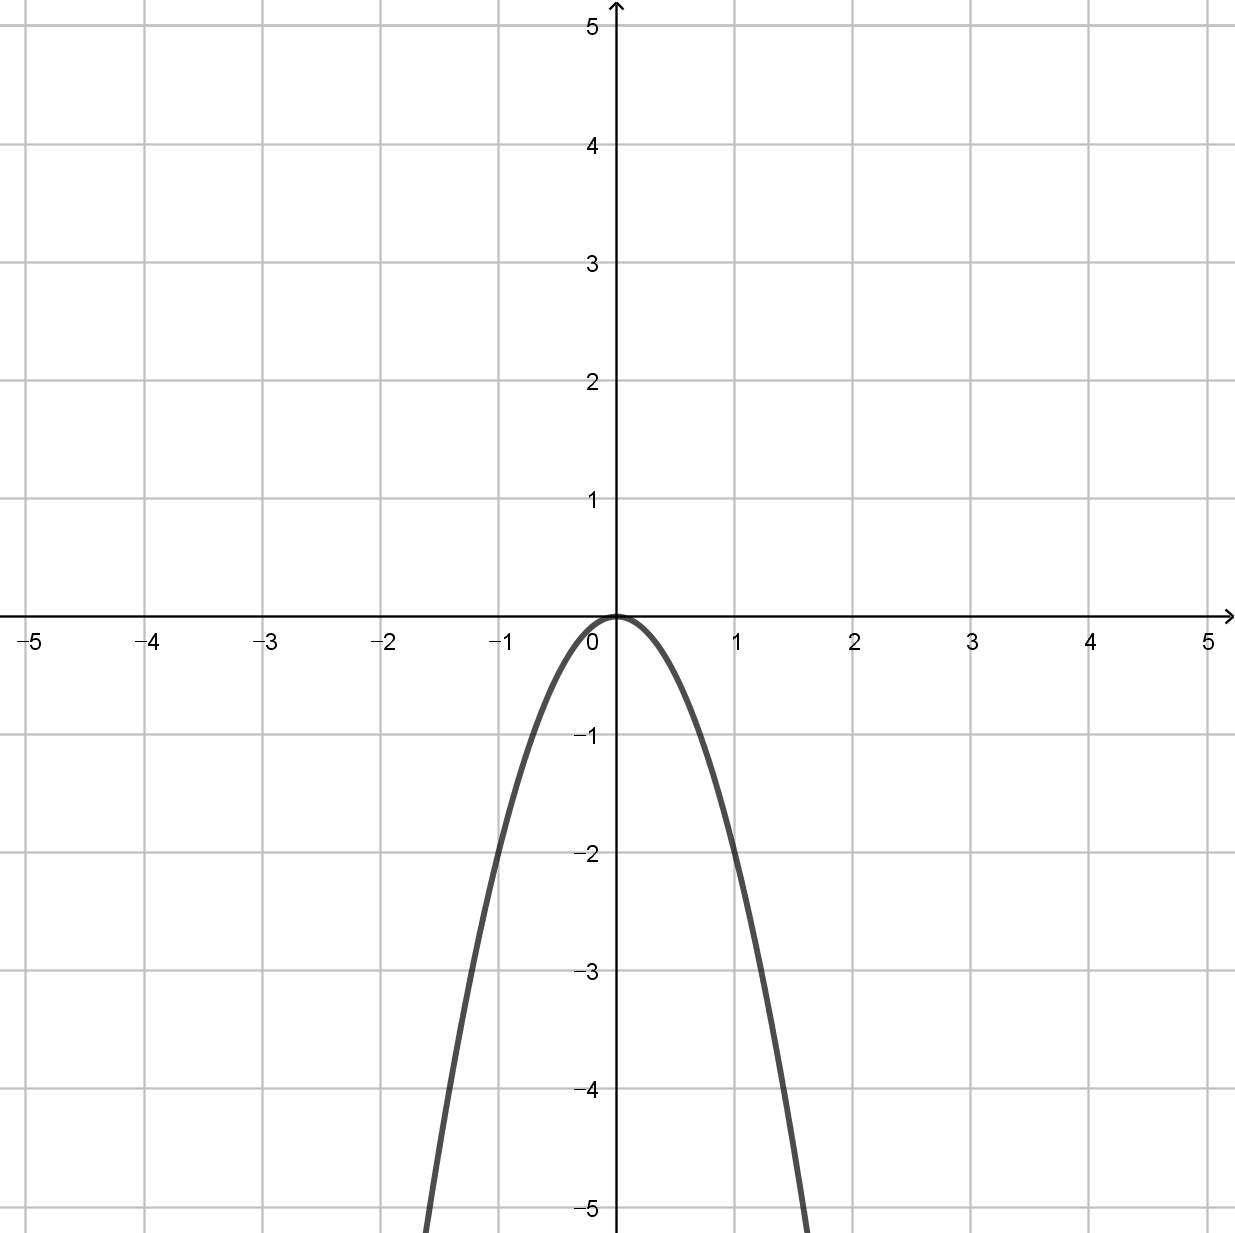
\includegraphics[width=0.9\textwidth]{img/2_quadratic_4}
\end{minipage}\bigskip\bigskip\par


\clearpage
\begin{minipage}{0.45\textwidth}\centering
\(y=3x^2\)
\par\bigskip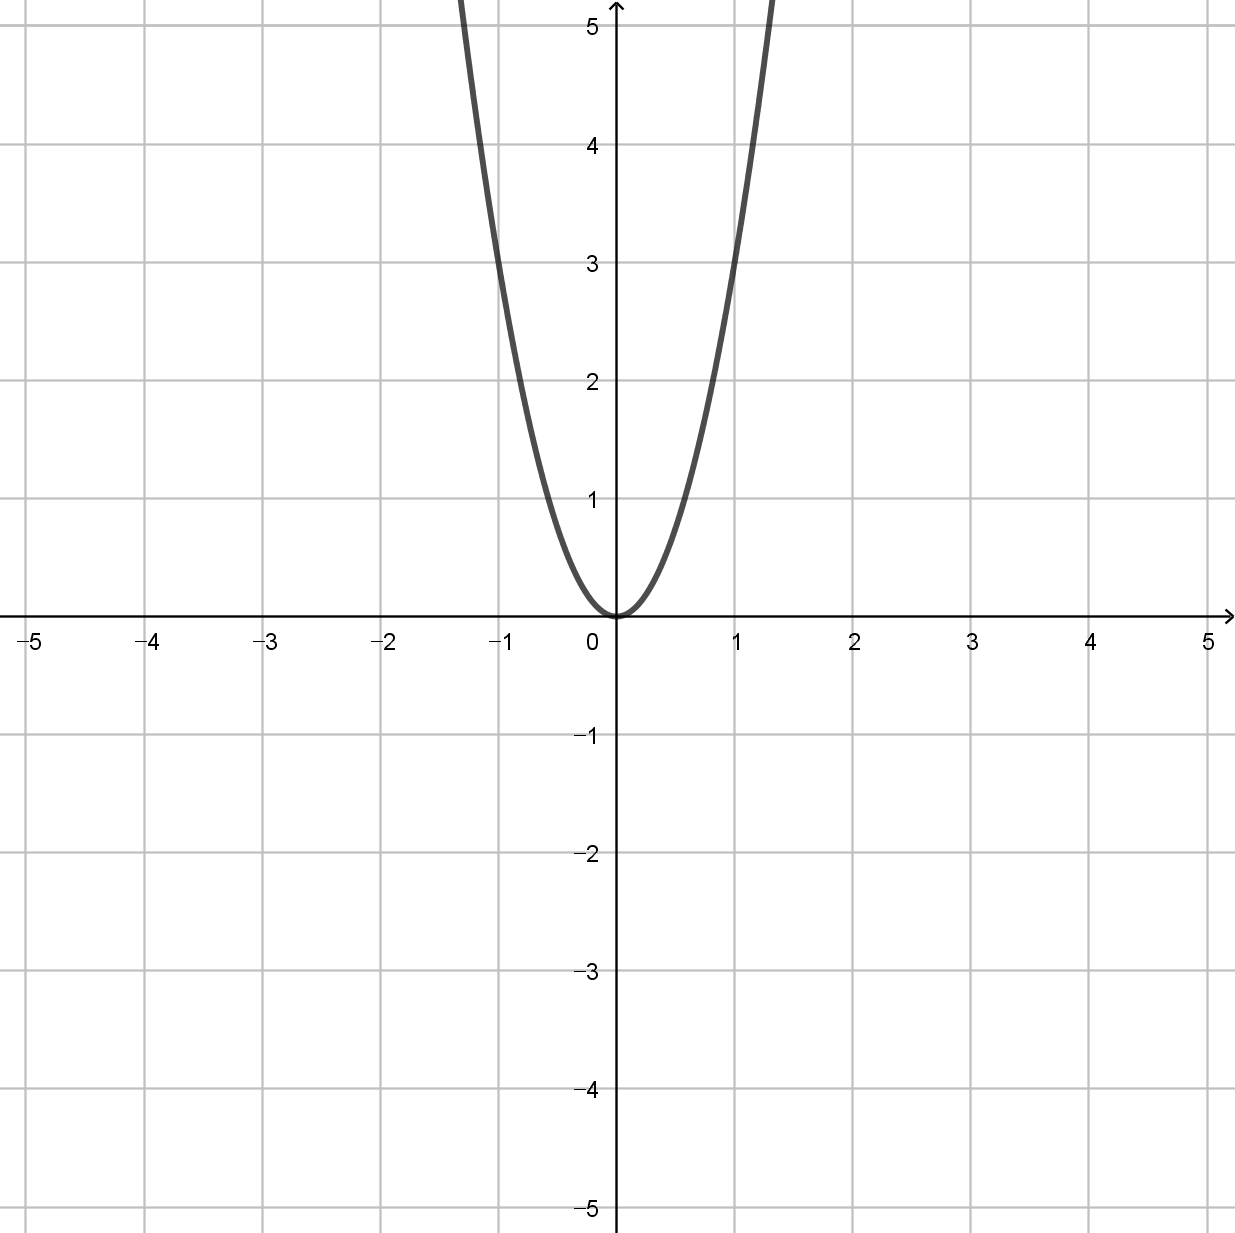
\includegraphics[width=0.9\textwidth]{img/2_quadratic_5}
\end{minipage}
\begin{minipage}{0.45\textwidth}\centering
\(y=-3x^2\)
\par\bigskip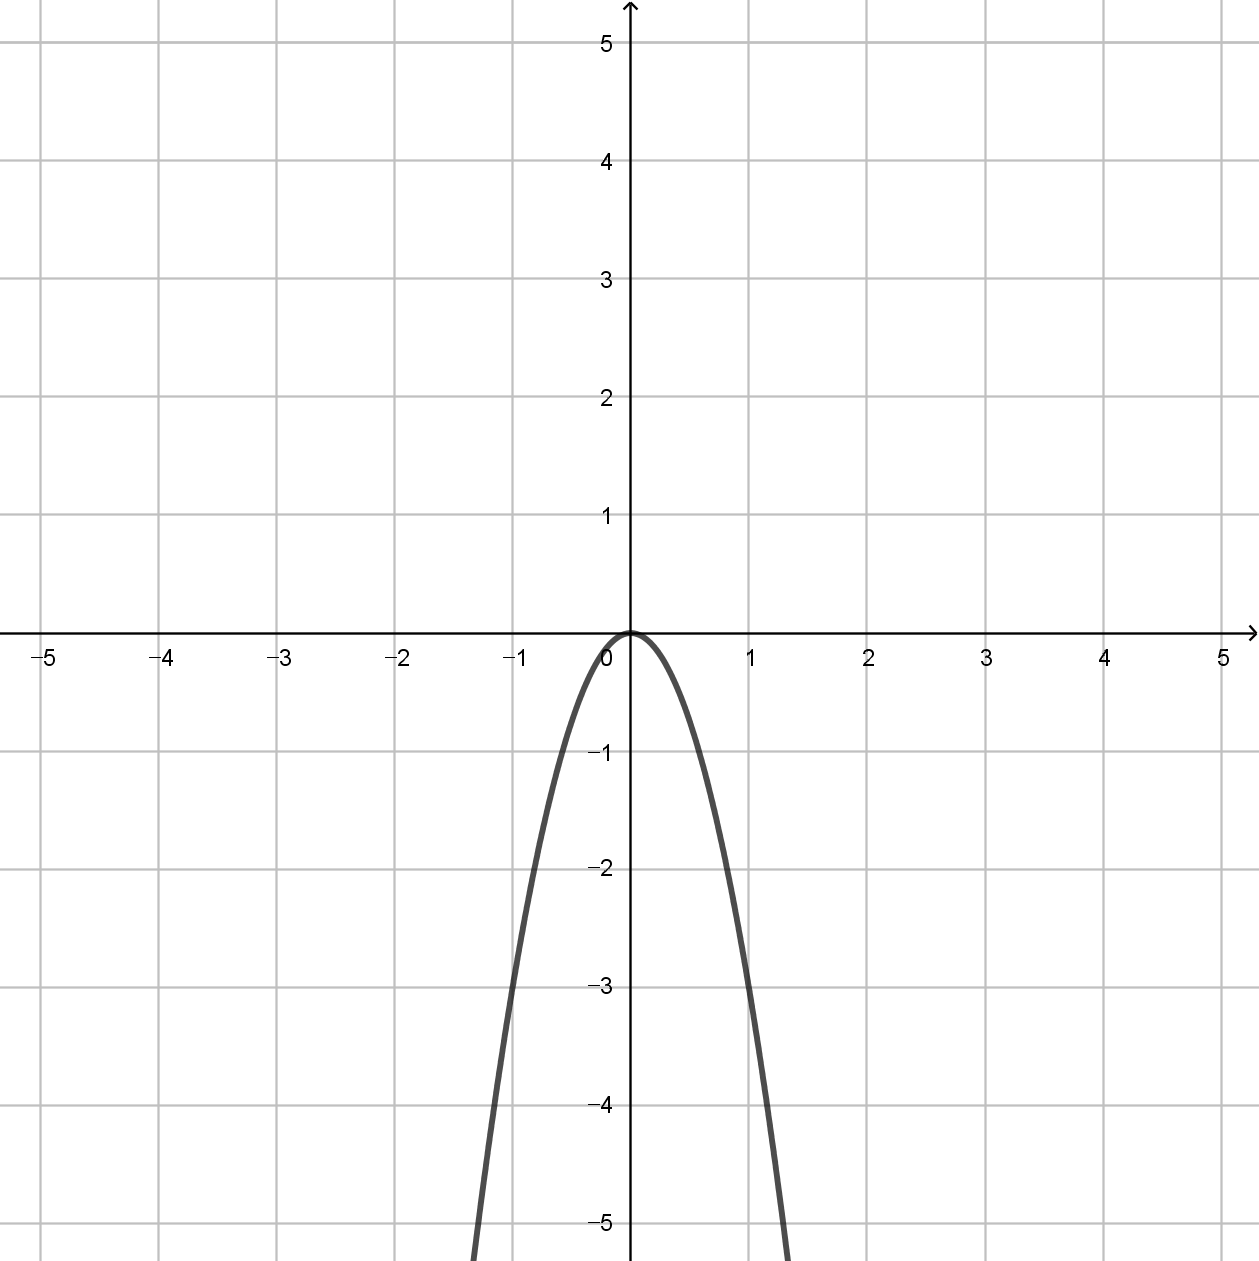
\includegraphics[width=0.9\textwidth]{img/2_quadratic_6}
\end{minipage}\bigskip\bigskip\par
\begin{minipage}{0.45\textwidth}\centering
\(y=\frac12x^2\)
\par\bigskip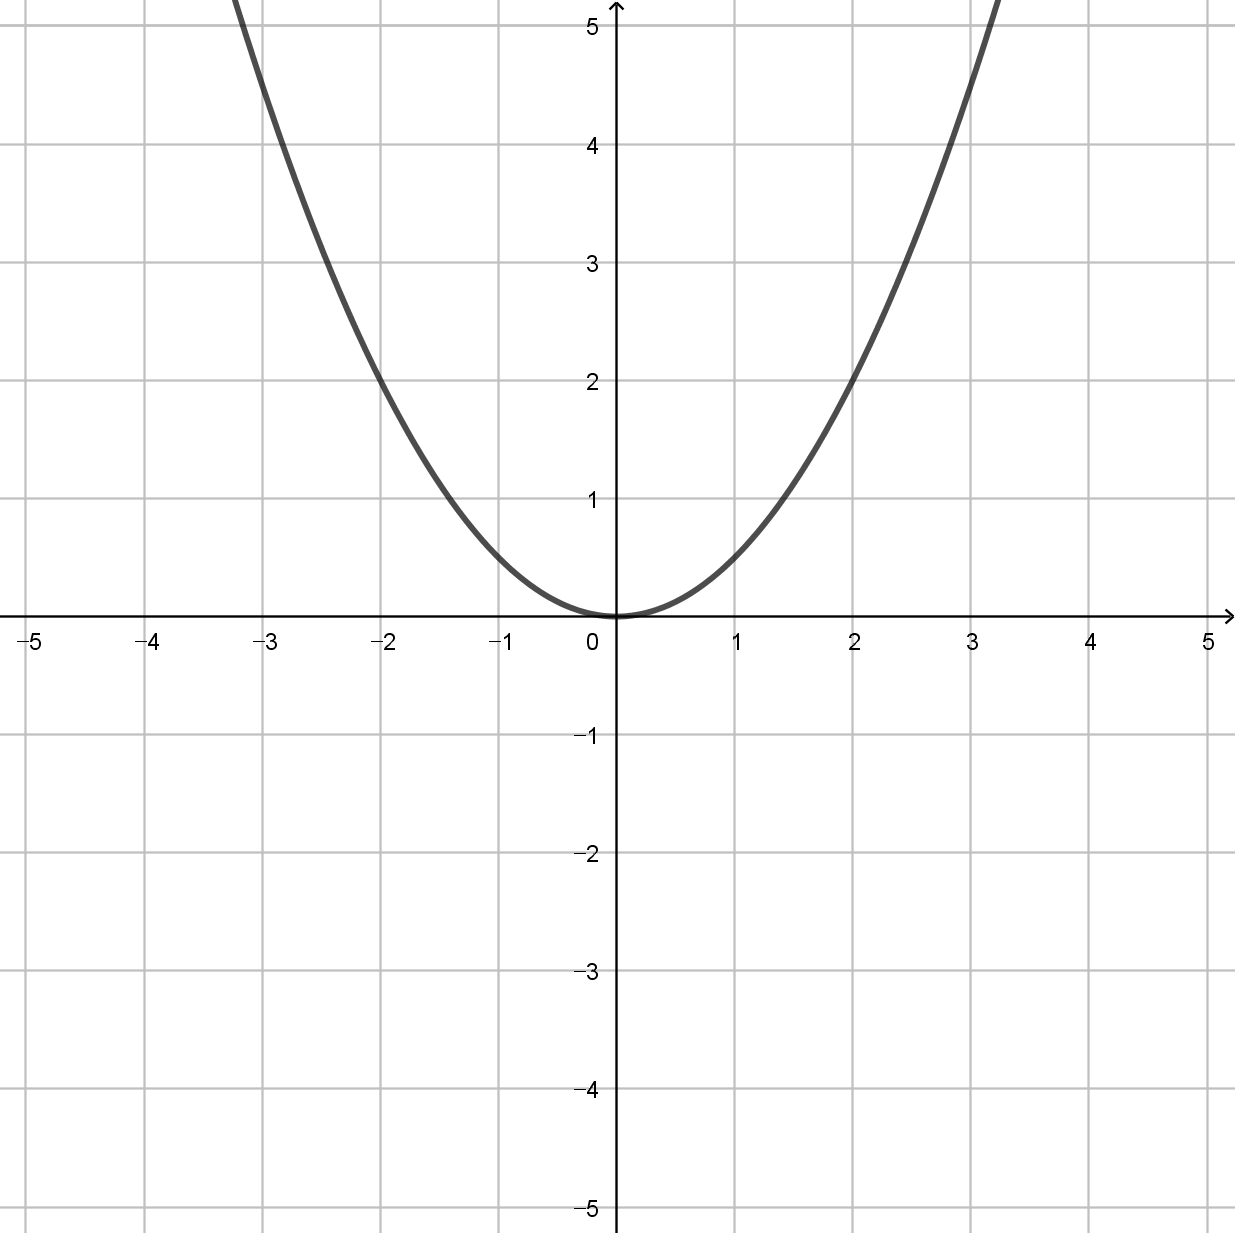
\includegraphics[width=0.9\textwidth]{img/2_quadratic_7}
\end{minipage}
\begin{minipage}{0.45\textwidth}\centering
\(y=-\frac12x^2\)
\par\bigskip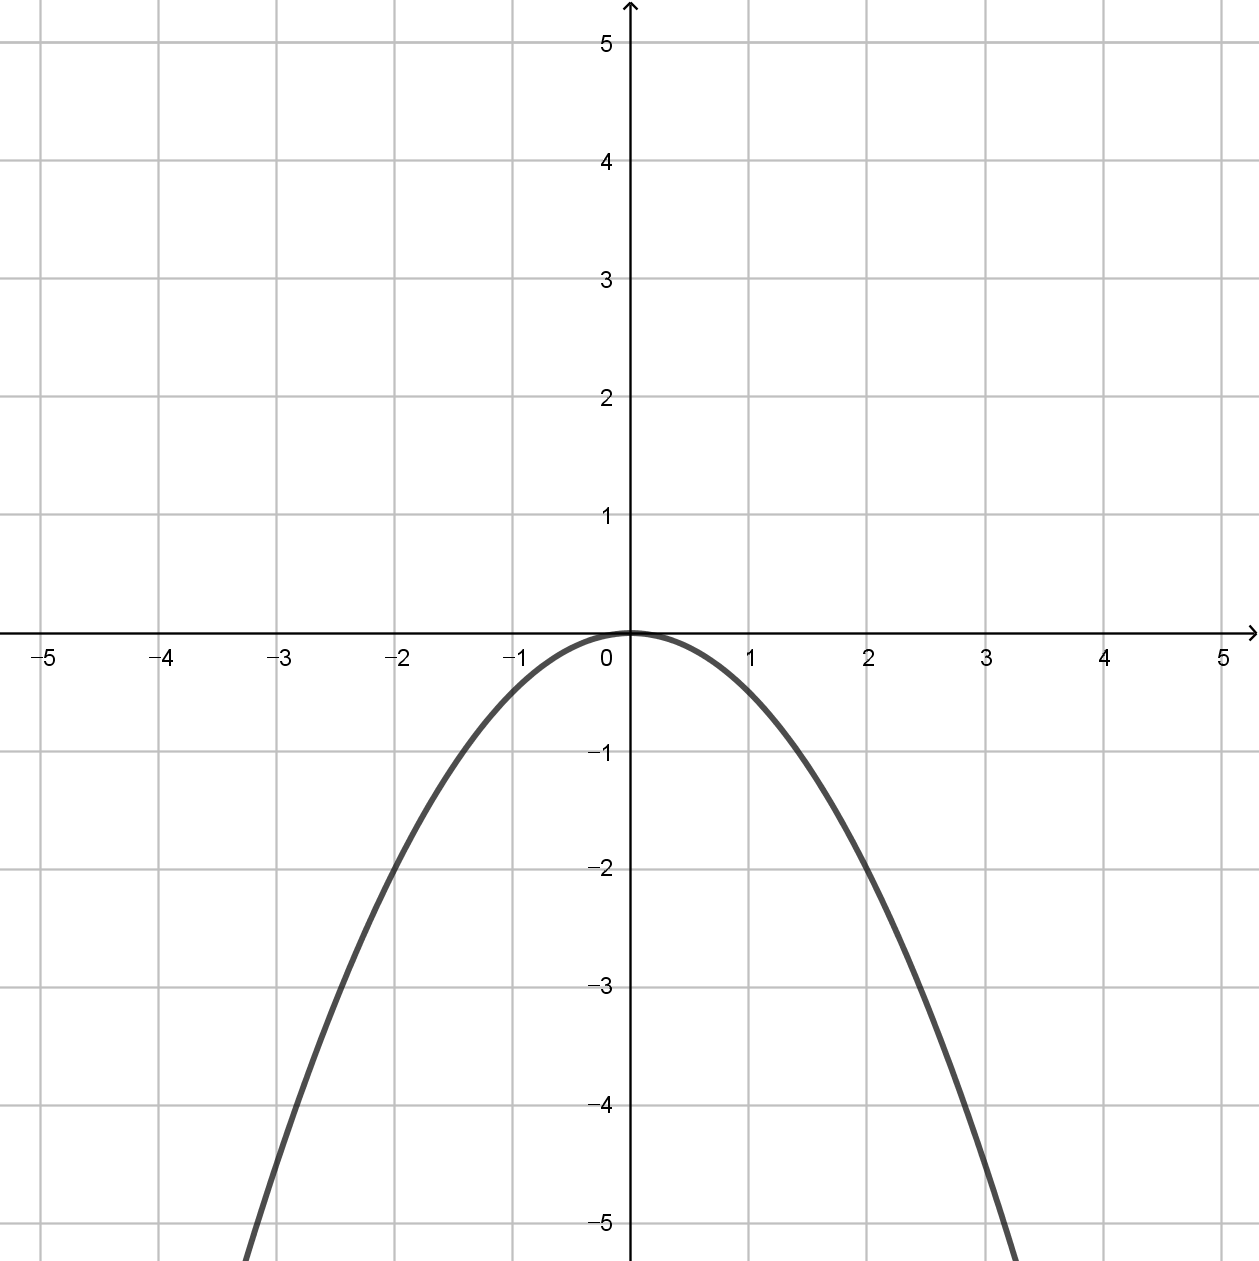
\includegraphics[width=0.9\textwidth]{img/2_quadratic_8}
\end{minipage}\bigskip\bigskip\par
\begin{minipage}{0.45\textwidth}\centering
\(y=x^2+1\)
\par\bigskip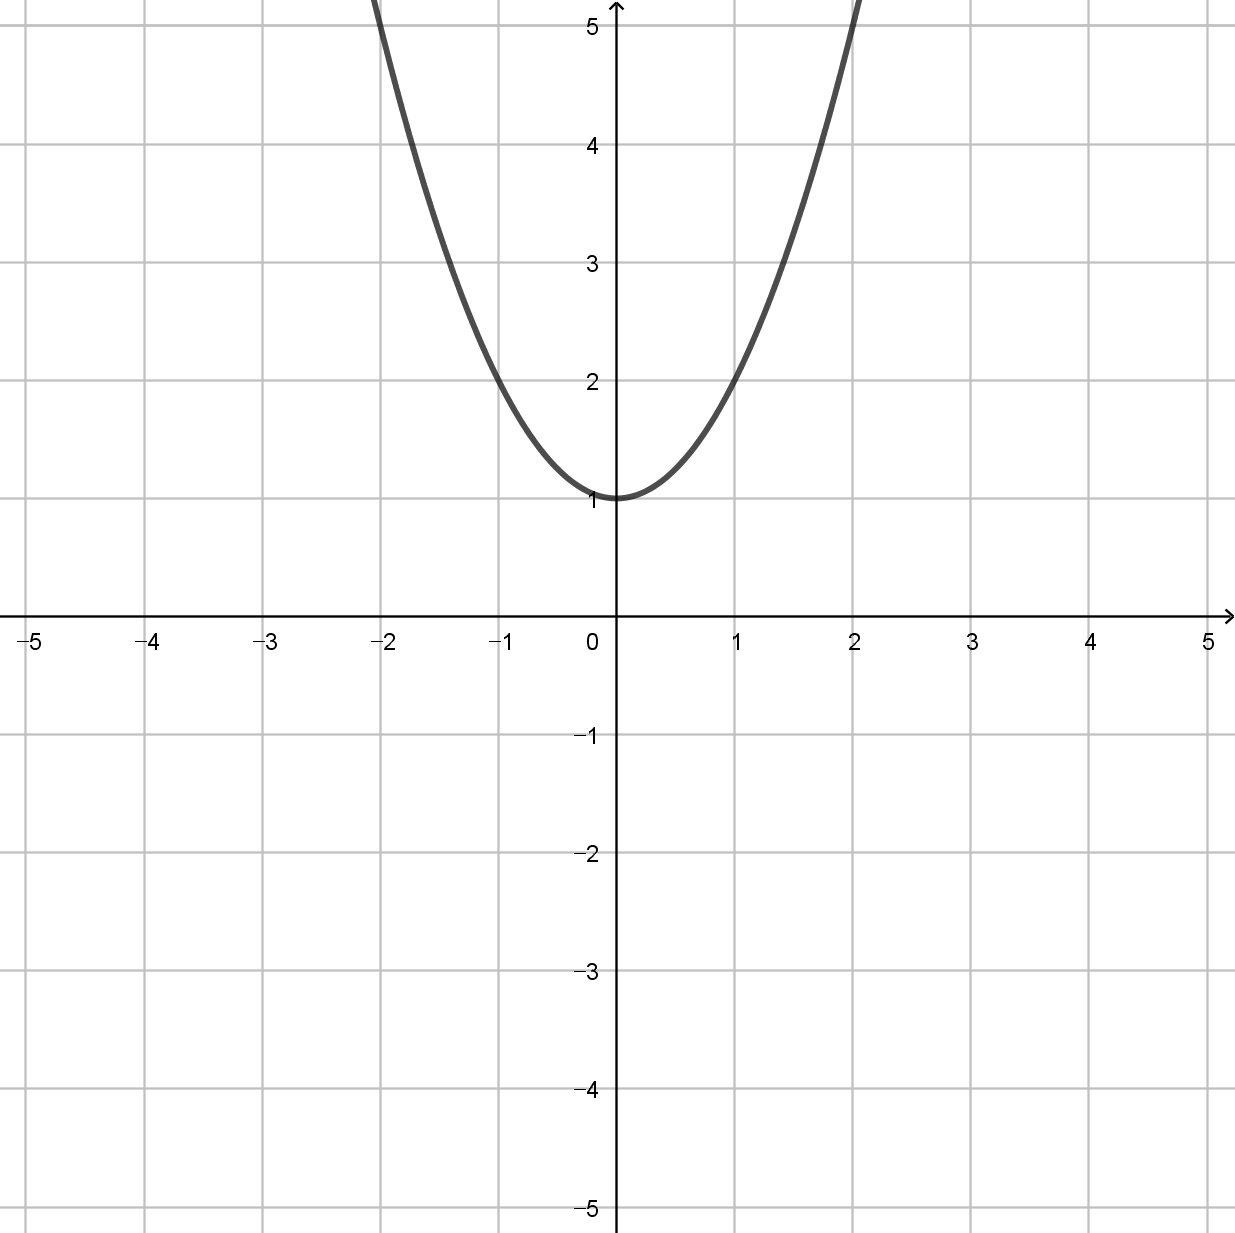
\includegraphics[width=0.9\textwidth]{img/2_quadratic_9}
\end{minipage}
\begin{minipage}{0.45\textwidth}\centering
\(y=x^2-2\)
\par\bigskip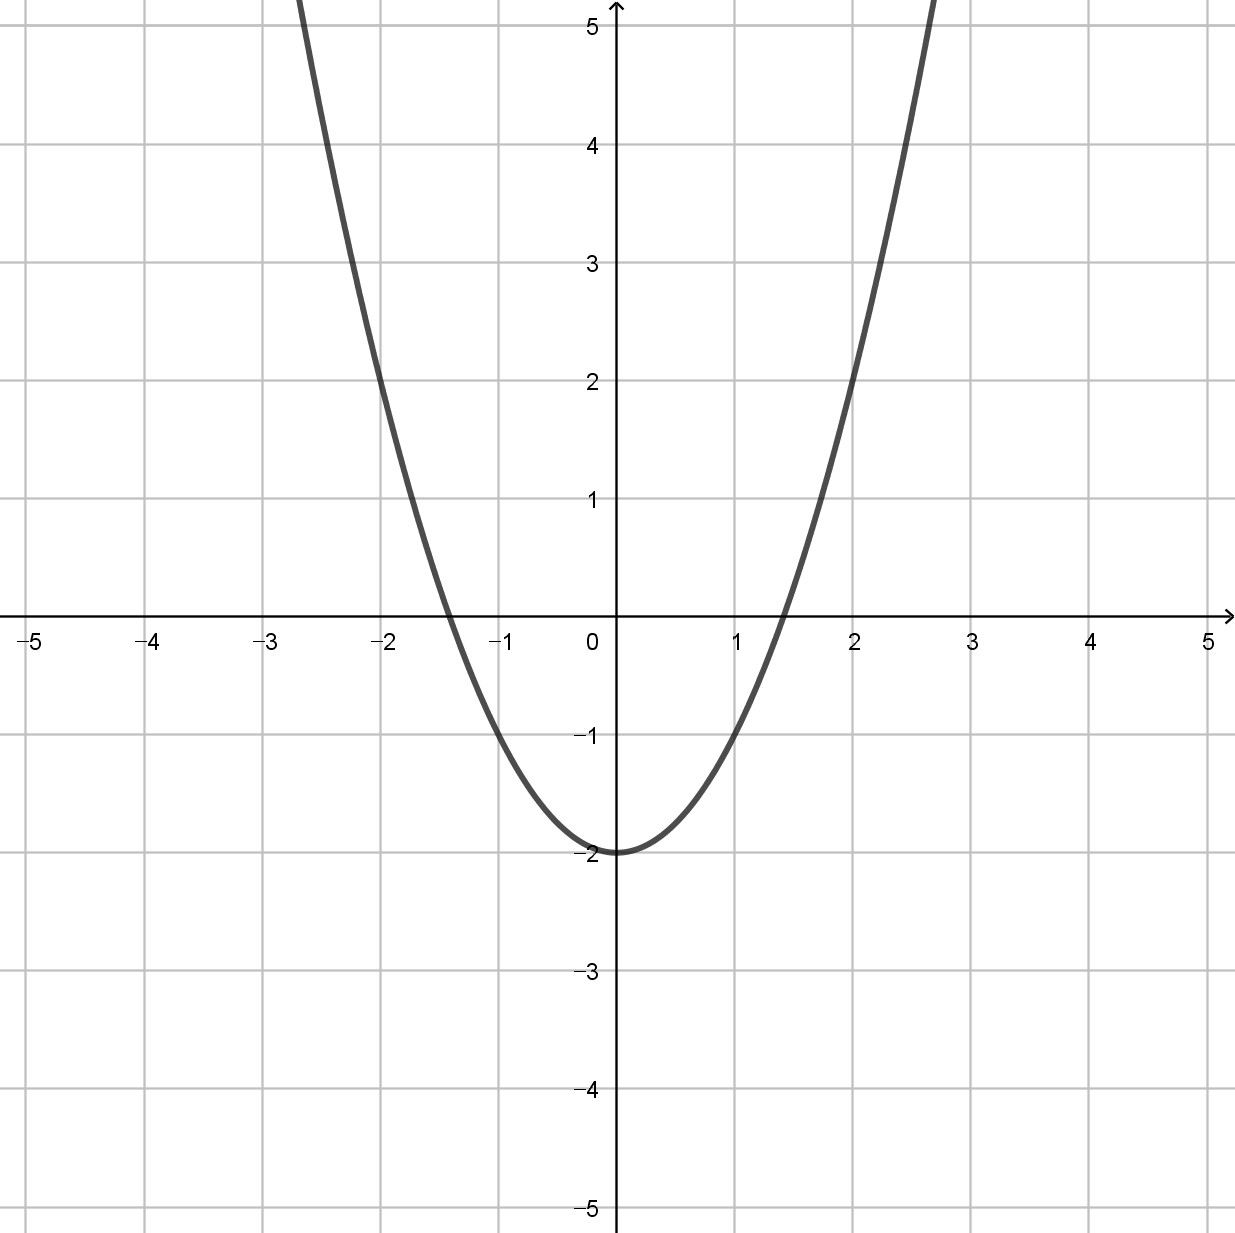
\includegraphics[width=0.9\textwidth]{img/2_quadratic_10}
\end{minipage}\bigskip\bigskip\par


\clearpage
\begin{minipage}{0.45\textwidth}\centering
\(y=-x^2+3\)
\par\bigskip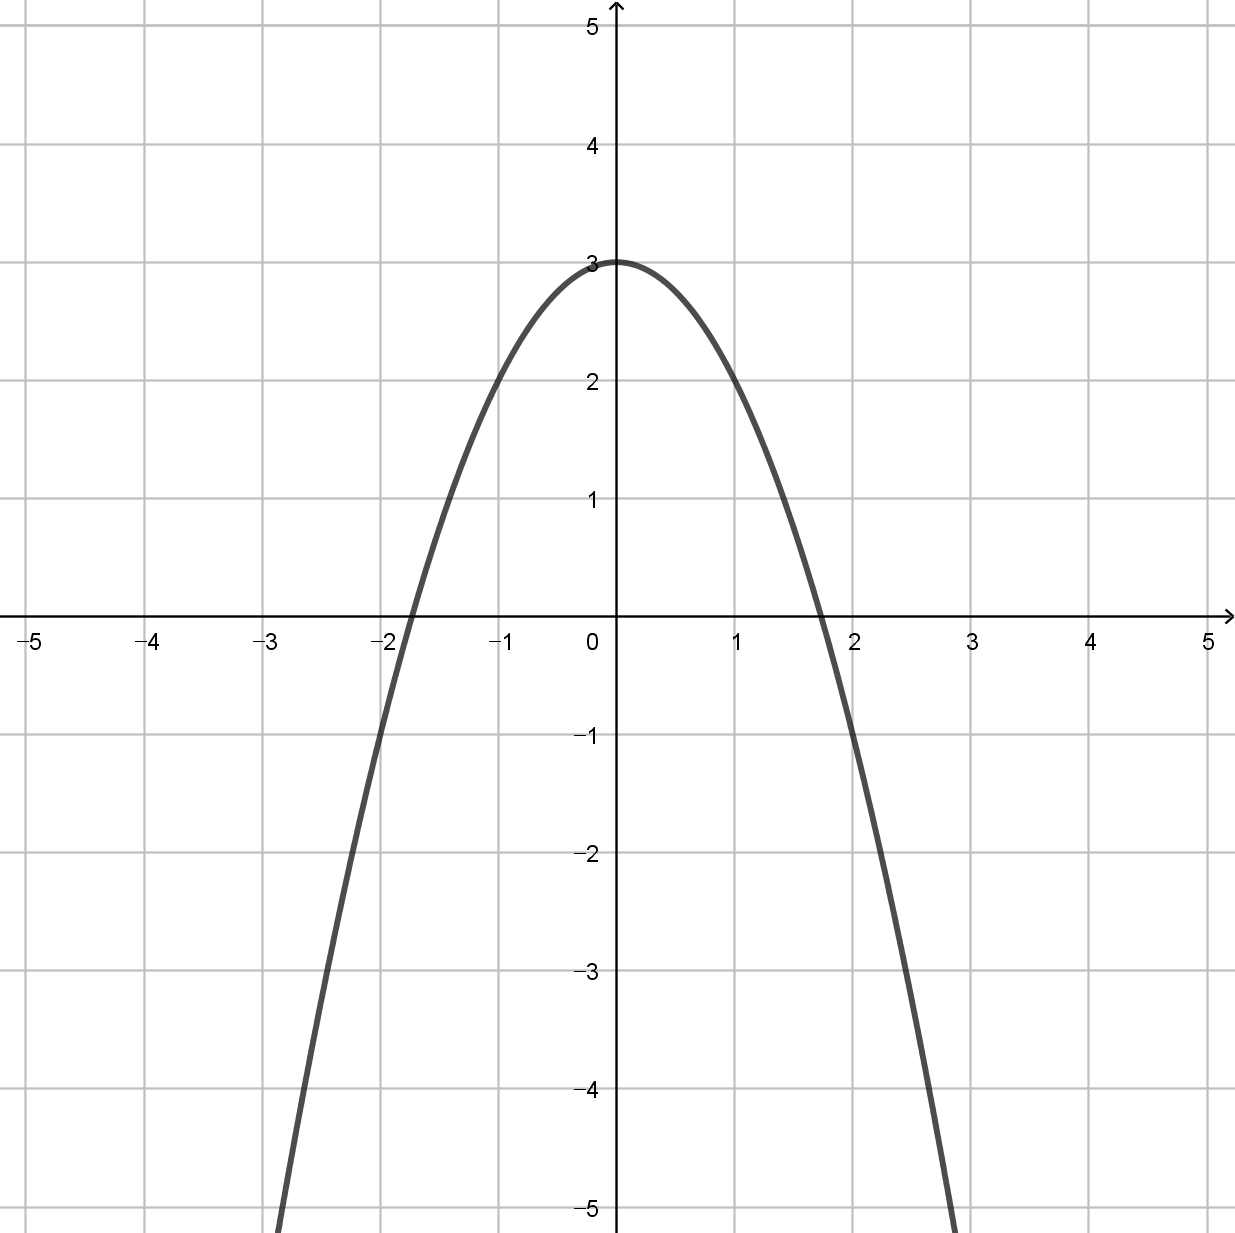
\includegraphics[width=0.9\textwidth]{img/2_quadratic_11}
\end{minipage}
\begin{minipage}{0.45\textwidth}\centering
\(y=4-x^2\)
\par\bigskip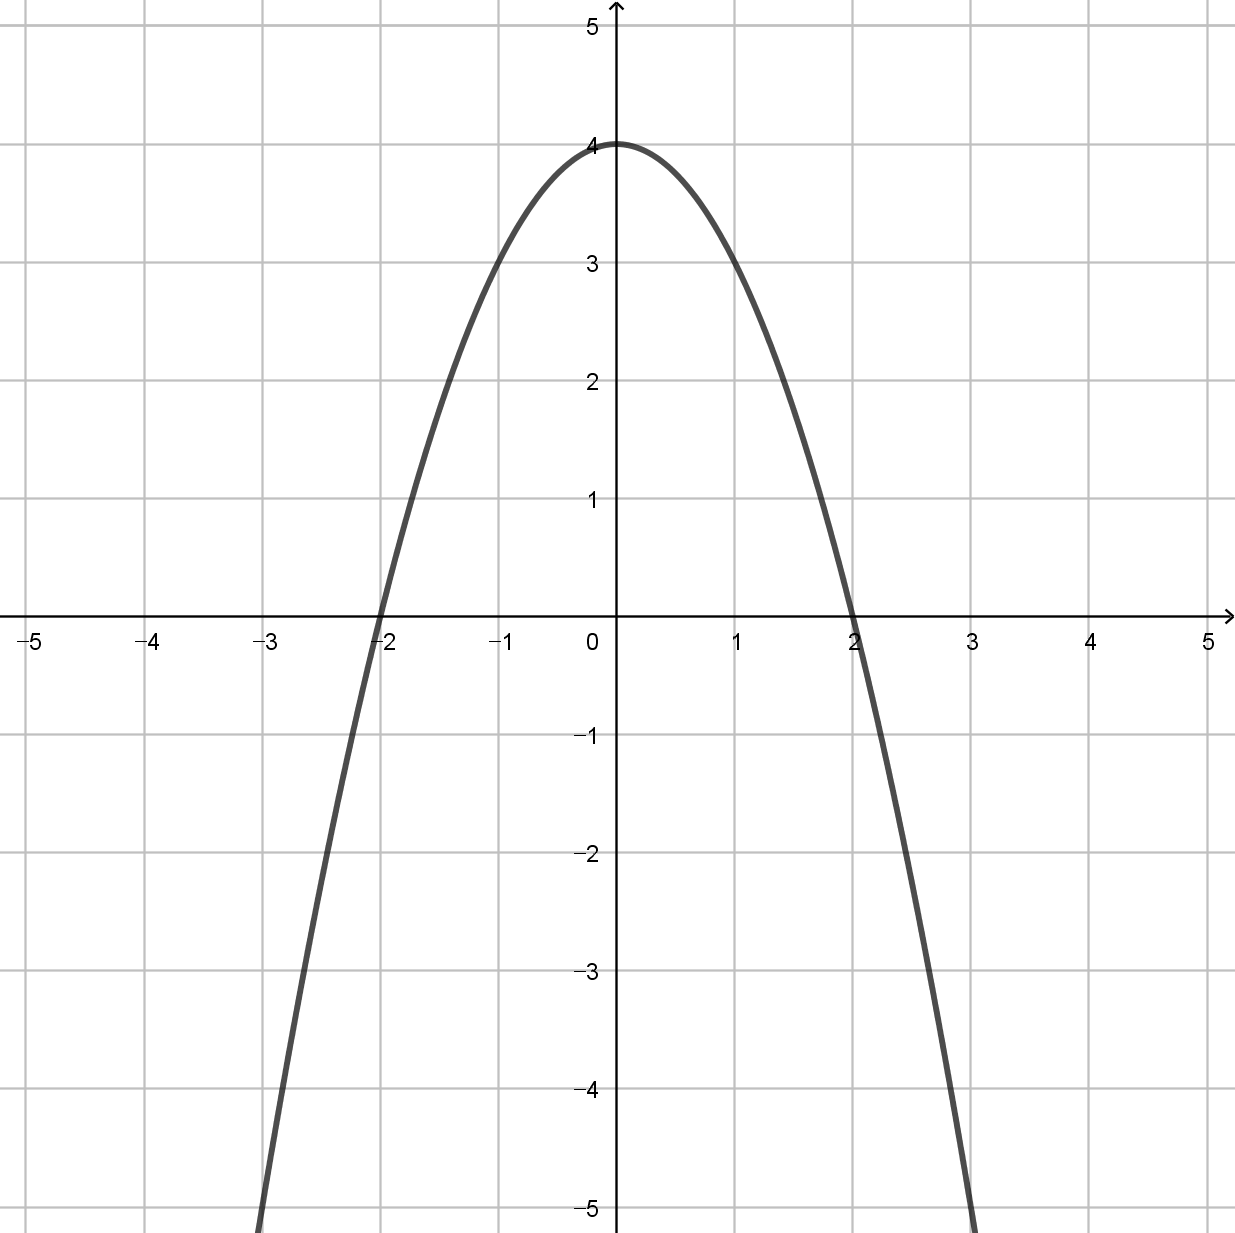
\includegraphics[width=0.9\textwidth]{img/2_quadratic_12}
\end{minipage}\bigskip\bigskip\par
\begin{minipage}{0.45\textwidth}\centering
\(y=2x^2-4\)
\par\bigskip\includegraphics[width=0.9\textwidth]{img/2_quadratic_13}
\end{minipage}
\begin{minipage}{0.45\textwidth}\centering
\(y=(x-1)^2\)
\par\bigskip\includegraphics[width=0.9\textwidth]{img/2_quadratic_14}
\end{minipage}\bigskip\bigskip\par
\begin{minipage}{0.45\textwidth}\centering
\(y=(x+2)^2\)
\par\bigskip\includegraphics[width=0.9\textwidth]{img/2_quadratic_15}
\end{minipage}
\begin{minipage}{0.45\textwidth}\centering
\(y=2(x-2)^2\)
\par\bigskip\includegraphics[width=0.9\textwidth]{img/2_quadratic_16}
\end{minipage}\bigskip\bigskip\par

\clearpage
\begin{minipage}{0.45\textwidth}\centering
\(y=(x-1)^2+2\)
\par\bigskip\includegraphics[width=0.9\textwidth]{img/2_quadratic_17}
\end{minipage}
\begin{minipage}{0.45\textwidth}\centering
\(y=2(x+3)^2-1\)
\par\bigskip\includegraphics[width=0.9\textwidth]{img/2_quadratic_18}
\end{minipage}\bigskip\bigskip\par
\begin{minipage}{0.45\textwidth}\centering
\(y=-(x-2)^2+4\)
\par\bigskip\includegraphics[width=0.9\textwidth]{img/2_quadratic_19}
\end{minipage}
\begin{minipage}{0.45\textwidth}\centering
\(y=\frac12(x+2)^2+1\)
\par\bigskip\includegraphics[width=0.9\textwidth]{img/2_quadratic_20}
\end{minipage}\bigskip\bigskip\par

\clearpage
\begin{minipage}{0.45\textwidth}\centering
\(y=x^2+2x+1\)
\par\bigskip\includegraphics[width=0.9\textwidth]{img/2_quadratic_21}
\end{minipage}
\begin{minipage}{0.45\textwidth}\centering
\(y=-x^2+4x-4\)
\par\bigskip\includegraphics[width=0.9\textwidth]{img/2_quadratic_22}
\end{minipage}\bigskip\bigskip\par
\begin{minipage}{0.45\textwidth}\centering
\(y=x^2-4x+2\)
\par\bigskip\includegraphics[width=0.9\textwidth]{img/2_quadratic_23}
\end{minipage}
\begin{minipage}{0.45\textwidth}\centering
\(y=x^2+4x+3\)
\par\bigskip\includegraphics[width=0.9\textwidth]{img/2_quadratic_24}
\end{minipage}\bigskip\bigskip\par
\begin{minipage}{0.45\textwidth}\centering
\(y=x^2+6x+5\)
\par\bigskip\includegraphics[width=0.9\textwidth]{img/2_quadratic_25}
\end{minipage}
\begin{minipage}{0.45\textwidth}\centering
\(y=x^2-2x-3\)
\par\bigskip\includegraphics[width=0.9\textwidth]{img/2_quadratic_26}
\end{minipage}\bigskip\bigskip\par

\clearpage
\begin{minipage}{0.45\textwidth}\centering
\(y=-x^2+2x-3\)
\par\bigskip\includegraphics[width=0.9\textwidth]{img/2_quadratic_27}
\end{minipage}
\begin{minipage}{0.45\textwidth}\centering
\(y=-x^2+4x-5\)
\par\bigskip\includegraphics[width=0.9\textwidth]{img/2_quadratic_28}
\end{minipage}\bigskip\bigskip\par
\begin{minipage}{0.45\textwidth}\centering
\(y=x^2-4x\)
\par\bigskip\includegraphics[width=0.9\textwidth]{img/2_quadratic_29}
\end{minipage}
\begin{minipage}{0.45\textwidth}\centering
\(y=-x^2+2x\)
\par\bigskip\includegraphics[width=0.9\textwidth]{img/2_quadratic_30}
\end{minipage}\bigskip\bigskip\par
\begin{minipage}{0.45\textwidth}\centering
\(y=2x^2-4x+4\)
\par\bigskip\includegraphics[width=0.9\textwidth]{img/2_quadratic_31}
\end{minipage}
\begin{minipage}{0.45\textwidth}\centering
\(y=2x^2+8x+5\)
\par\bigskip\includegraphics[width=0.9\textwidth]{img/2_quadratic_32}
\end{minipage}\bigskip\bigskip\par

\clearpage
\begin{minipage}{0.45\textwidth}\centering
\(y=-2x^2-4x\)
\par\bigskip\includegraphics[width=0.9\textwidth]{img/2_quadratic_33}
\end{minipage}
\begin{minipage}{0.45\textwidth}\centering
\(y=-2x^2+12x-16\)
\par\bigskip\includegraphics[width=0.9\textwidth]{img/2_quadratic_34}
\end{minipage}\bigskip\bigskip\par
\begin{minipage}{0.45\textwidth}\centering
\(y=3x^2-6x-1\)
\par\bigskip\includegraphics[width=0.9\textwidth]{img/2_quadratic_35}
\end{minipage}
\begin{minipage}{0.45\textwidth}\centering
\(y=-3x^2-12x-10\)
\par\bigskip\includegraphics[width=0.9\textwidth]{img/2_quadratic_36}
\end{minipage}\bigskip\bigskip\par
\begin{minipage}{0.45\textwidth}\centering
\(y=\frac12x^2-2x+3\)
\par\bigskip\includegraphics[width=0.9\textwidth]{img/2_quadratic_37}
\end{minipage}
\begin{minipage}{0.45\textwidth}\centering
\(y=-\frac12x^2+4x-6\)
\par\bigskip\includegraphics[width=0.9\textwidth]{img/2_quadratic_38}
\end{minipage}\bigskip\bigskip\par

\end{document}